%%%%%%%%%%%%%%%%%%%%%%%%%%%%%%%%%%%%%%%%%
% The Legrand Orange Book
% LaTeX Template
% Version 1.4 (12/4/14)
%
% This template has been downloaded from:
% http://www.LaTeXTemplates.com
%
% Original author:
% Mathias Legrand (legrand.mathias@gmail.com)
%
% License:
% CC BY-NC-SA 3.0 (http://creativecommons.org/licenses/by-nc-sa/3.0/)
%
% Compiling this template:
% This template uses biber for its bibliography and makeindex for its index.
% When you first open the template, compile it from the command line with the 
% commands below to make sure your LaTeX distribution is configured correctly:
%
% 1) pdflatex oqhbt
% 2) makeindex oqhbt.idx -s StyleInd.ist
% 3) biber oqhbt
% 4  makeglossaries oqhbt
% 4) pdflatex oqhbt x 2
%
% After this, when you wish to update the bibliography/index use the appropriate
% command above and make sure to compile with pdflatex several times 
% afterwards to propagate your changes to the document.
%
% This template also uses a number of packages which may need to be
% updated to the newest versions for the template to compile. It is strongly
% recommended you update your LaTeX distribution if you have any
% compilation errors.
%
% Important note:
% Chapter heading images should have a 2:1 width:height ratio,
% e.g. 920px width and 460px height.
%
%%%%%%%%%%%%%%%%%%%%%%%%%%%%%%%%%%%%%%%%%

%----------------------------------------------------------------------------------------
%	PACKAGES AND OTHER DOCUMENT CONFIGURATIONS
%----------------------------------------------------------------------------------------

\documentclass[11pt,fleqn]{book} % Default font size and left-justified equations

\usepackage[top=3cm,bottom=3cm,left=3.2cm,right=3.2cm,headsep=10pt,a4paper]{geometry} % Page margins

\usepackage{xcolor} % Required for specifying colors by name
\definecolor{ocre}{RGB}{243,102,25} % Define the orange color used for highlighting throughout the book

% Font Settings
\usepackage{avant} % Use the Avantgarde font for headings
%\usepackage{times} % Use the Times font for headings
\usepackage{mathptmx} % Use the Adobe Times Roman as the default text font together with math symbols from the Sym­bol, Chancery and Com­puter Modern fonts

\usepackage{microtype} % Slightly tweak font spacing for aesthetics
\usepackage[utf8]{inputenc} % Required for including letters with accents
\usepackage[T1]{fontenc} % Use 8-bit encoding that has 256 glyphs

% Bibliography
\usepackage[style=alphabetic,
            sorting=nyt,
            sortcites=true,
            natbib=true,
            style=authoryear,
            maxcitenames=2,
            maxbibnames=100,
            autopunct=true,
            babel=hyphen,
            hyperref=true,
            doi=true,
            abbreviate=false,
            backref=true,
            backend=biber]{biblatex}
\addbibresource{./Bibliography/hazard.bib} % BibTeX bibliography file
\defbibheading{bibempty}{}

% Figure caption settings
\usepackage[textfont=it,margin=10pt,font=small,labelfont=bf,labelsep=endash]{caption}

% Table
\usepackage{color, colortbl}
\definecolor{almond}{rgb}{0.94, 0.87, 0.8}
\definecolor{ashgrey}{rgb}{0.7, 0.75, 0.71}
\definecolor{anti-flashwhite}{rgb}{0.95, 0.95, 0.96}

% Index
\usepackage{calc} % For simpler calculation - used for spacing the index letter headings correctly
\usepackage{makeidx} % Required to make an index
\makeindex % Tells LaTeX to create the files required for indexing

\usepackage{todonotes}

%
% Package to create a glossary - It must be uploaded after hyperref
% to produce the glossary: makeglossaries OQB
\usepackage[acronym,nonumberlist,style=altlist]{glossaries}
\glstoctrue
\makeglossaries

% package for bold symbols
\usepackage{bm}

%----------------------------------------------------------------------------------------
% Insert the commands.tex file which contains the majority of the structure 
% behind the template
%----------------------------------------------------------------------------------------
%	VARIOUS REQUIRED PACKAGES
%----------------------------------------------------------------------------------------

\usepackage{titlesec} % Allows customization of titles

\usepackage{graphicx} % Required for including pictures
\graphicspath{{Pictures/}} % Specifies the directory where pictures are stored

\usepackage{tikz} % Required for drawing custom shapes

\usepackage[english]{babel} % English language/hyphenation

\usepackage{enumitem} % Customize lists
\setlist{nolistsep} % Reduce spacing between bullet points and numbered lists

\usepackage{booktabs} % Required for nicer horizontal rules in tables

\usepackage{eso-pic} % Required for specifying an image background in the title page

%----------------------------------------------------------------------------------------
%	MAIN TABLE OF CONTENTS
%----------------------------------------------------------------------------------------

\usepackage{titletoc} % Required for manipulating the table of contents

\contentsmargin{0cm} % Removes the default margin
% Chapter text styling
\titlecontents{chapter}[1.25cm] % Indentation
{\addvspace{15pt}\large\sffamily\bfseries} % Spacing and font options for chapters
{\color{ocre!60}\contentslabel[\Large\thecontentslabel]{1.25cm}\color{ocre}} % Chapter number
{}  
{\color{ocre!60}\normalsize\sffamily\bfseries\;\titlerule*[.5pc]{.}\;\thecontentspage} % Page number
% Section text styling
\titlecontents{section}[1.25cm] % Indentation
{\addvspace{5pt}\sffamily\bfseries} % Spacing and font options for sections
{\contentslabel[\thecontentslabel]{1.25cm}} % Section number
{}
{\sffamily\hfill\color{black}\thecontentspage} % Page number
[]
% Subsection text styling
\titlecontents{subsection}[1.25cm] % Indentation
{\addvspace{1pt}\sffamily\small} % Spacing and font options for subsections
{\contentslabel[\thecontentslabel]{1.25cm}} % Subsection number
{}
{\sffamily\;\titlerule*[.5pc]{.}\;\thecontentspage} % Page number
[] 

%----------------------------------------------------------------------------------------
%	MINI TABLE OF CONTENTS IN CHAPTER HEADS
%----------------------------------------------------------------------------------------

% Section text styling
\titlecontents{lsection}[0em] % Indendating
{\footnotesize\sffamily} % Font settings
{}
{}
{}

% Subsection text styling
\titlecontents{lsubsection}[.5em] % Indentation
{\normalfont\footnotesize\sffamily} % Font settings
{}
{}
{}
 
%----------------------------------------------------------------------------------------
%	PAGE HEADERS
%----------------------------------------------------------------------------------------

\usepackage{fancyhdr} % Required for header and footer configuration

\pagestyle{fancy}
\renewcommand{\chaptermark}[1]{\markboth{\sffamily\normalsize\bfseries\chaptername\ \thechapter.\ #1}{}} % Chapter text font settings
\renewcommand{\sectionmark}[1]{\markright{\sffamily\normalsize\thesection\hspace{5pt}#1}{}} % Section text font settings
\fancyhf{} \fancyhead[LE,RO]{\sffamily\normalsize\thepage} % Font setting for the page number in the header
\fancyhead[LO]{\rightmark} % Print the nearest section name on the left side of odd pages
\fancyhead[RE]{\leftmark} % Print the current chapter name on the right side of even pages
\renewcommand{\headrulewidth}{0.5pt} % Width of the rule under the header
\addtolength{\headheight}{2.5pt} % Increase the spacing around the header slightly
\renewcommand{\footrulewidth}{0pt} % Removes the rule in the footer
\fancypagestyle{plain}{\fancyhead{}\renewcommand{\headrulewidth}{0pt}} % Style for when a plain pagestyle is specified

% Removes the header from odd empty pages at the end of chapters
\makeatletter
\renewcommand{\cleardoublepage}{
\clearpage\ifodd\c@page\else
\hbox{}
\vspace*{\fill}
\thispagestyle{empty}
\newpage
\fi}

%----------------------------------------------------------------------------------------
%	THEOREM STYLES
%----------------------------------------------------------------------------------------

\usepackage{amsmath,amsfonts,amssymb,amsthm} % For math equations, theorems, symbols, etc

\newcommand{\intoo}[2]{\mathopen{]}#1\,;#2\mathclose{[}}
\newcommand{\ud}{\mathop{\mathrm{{}d}}\mathopen{}}
\newcommand{\intff}[2]{\mathopen{[}#1\,;#2\mathclose{]}}
\newtheorem{notation}{Notation}[chapter]

%%%%%%%%%%%%%%%%%%%%%%%%%%%%%%%%%%%%%%%%%%%%%%%%%%%%%%%%%%%%%%%%%%%%%%%%%%%
%%%%%%%%%%%%%%%%%%%% dedicated to boxed/framed environements %%%%%%%%%%%%%%
%%%%%%%%%%%%%%%%%%%%%%%%%%%%%%%%%%%%%%%%%%%%%%%%%%%%%%%%%%%%%%%%%%%%%%%%%%%
\newtheoremstyle{ocrenumbox}% % Theorem style name
{0pt}% Space above
{0pt}% Space below
{\normalfont}% % Body font
{}% Indent amount
{\small\bf\sffamily\color{ocre}}% % Theorem head font
{\;}% Punctuation after theorem head
{0.25em}% Space after theorem head
{\small\sffamily\color{ocre}\thmname{#1}\nobreakspace\thmnumber{\@ifnotempty{#1}{}\@upn{#2}}% Theorem text (e.g. Theorem 2.1)
\thmnote{\nobreakspace\the\thm@notefont\sffamily\bfseries\color{black}---\nobreakspace#3.}} % Optional theorem note
\renewcommand{\qedsymbol}{$\blacksquare$}% Optional qed square

\newtheoremstyle{blacknumex}% Theorem style name
{5pt}% Space above
{5pt}% Space below
{\normalfont}% Body font
{} % Indent amount
{\small\bf\sffamily}% Theorem head font
{\;}% Punctuation after theorem head
{0.25em}% Space after theorem head
{\small\sffamily{\tiny\ensuremath{\blacksquare}}\nobreakspace\thmname{#1}\nobreakspace\thmnumber{\@ifnotempty{#1}{}\@upn{#2}}% Theorem text (e.g. Theorem 2.1)
\thmnote{\nobreakspace\the\thm@notefont\sffamily\bfseries---\nobreakspace#3.}}% Optional theorem note

\newtheoremstyle{blacknumbox} % Theorem style name
{0pt}% Space above
{0pt}% Space below
{\normalfont}% Body font
{}% Indent amount
{\small\bf\sffamily}% Theorem head font
{\;}% Punctuation after theorem head
{0.25em}% Space after theorem head
{\small\sffamily\thmname{#1}\nobreakspace\thmnumber{\@ifnotempty{#1}{}\@upn{#2}}% Theorem text (e.g. Theorem 2.1)
\thmnote{\nobreakspace\the\thm@notefont\sffamily\bfseries---\nobreakspace#3.}}% Optional theorem note

%%%%%%%%%%%%%%%%%%%%%%%%%%%%%%%%%%%%%%%%%%%%%%%%%%%%%%%%%%%%%%%%%%%%%%%%%%%
%%%%%%%%%%%%% dedicated to non-boxed/non-framed environements %%%%%%%%%%%%%
%%%%%%%%%%%%%%%%%%%%%%%%%%%%%%%%%%%%%%%%%%%%%%%%%%%%%%%%%%%%%%%%%%%%%%%%%%%
\newtheoremstyle{ocrenum}% % Theorem style name
{5pt}% Space above
{5pt}% Space below
{\normalfont}% % Body font
{}% Indent amount
{\small\bf\sffamily\color{ocre}}% % Theorem head font
{\;}% Punctuation after theorem head
{0.25em}% Space after theorem head
{\small\sffamily\color{ocre}\thmname{#1}\nobreakspace\thmnumber{\@ifnotempty{#1}{}\@upn{#2}}% Theorem text (e.g. Theorem 2.1)
\thmnote{\nobreakspace\the\thm@notefont\sffamily\bfseries\color{black}---\nobreakspace#3.}} % Optional theorem note
\renewcommand{\qedsymbol}{$\blacksquare$}% Optional qed square
\makeatother

% Defines the theorem text style for each type of theorem to one of the three styles above
\newcounter{dummy} 
\numberwithin{dummy}{section}
\theoremstyle{ocrenumbox}
\newtheorem{theoremeT}[dummy]{Theorem}
\newtheorem{problem}{Problem}[chapter]
\newtheorem{exerciseT}{Exercise}[chapter]
\theoremstyle{blacknumex}
\newtheorem{exampleT}{Example}[chapter]
\theoremstyle{blacknumbox}
\newtheorem{vocabulary}{Vocabulary}[chapter]
\newtheorem{definitionT}{Definition}[section]
\newtheorem{corollaryT}[dummy]{Corollary}
\theoremstyle{ocrenum}
\newtheorem{proposition}[dummy]{Proposition}

%----------------------------------------------------------------------------------------
%	DEFINITION OF COLORED BOXES
%----------------------------------------------------------------------------------------

\RequirePackage[framemethod=default]{mdframed} % Required for creating the theorem, definition, exercise and corollary boxes

% Theorem box
\newmdenv[skipabove=7pt,
skipbelow=7pt,
backgroundcolor=black!5,
linecolor=ocre,
innerleftmargin=5pt,
innerrightmargin=5pt,
innertopmargin=5pt,
leftmargin=0cm,
rightmargin=0cm,
innerbottommargin=5pt]{tBox}

% Exercise box	  
\newmdenv[skipabove=7pt,
skipbelow=7pt,
rightline=false,
leftline=true,
topline=false,
bottomline=false,
backgroundcolor=ocre!10,
linecolor=ocre,
innerleftmargin=5pt,
innerrightmargin=5pt,
innertopmargin=5pt,
innerbottommargin=5pt,
leftmargin=0cm,
rightmargin=0cm,
linewidth=4pt]{eBox}	

% Definition box
\newmdenv[skipabove=7pt,
skipbelow=7pt,
rightline=false,
leftline=true,
topline=false,
bottomline=false,
linecolor=ocre,
innerleftmargin=5pt,
innerrightmargin=5pt,
innertopmargin=0pt,
leftmargin=0cm,
rightmargin=0cm,
linewidth=4pt,
innerbottommargin=0pt]{dBox}	

% Corollary box
\newmdenv[skipabove=7pt,
skipbelow=7pt,
rightline=false,
leftline=true,
topline=false,
bottomline=false,
linecolor=gray,
backgroundcolor=black!5,
innerleftmargin=5pt,
innerrightmargin=5pt,
innertopmargin=5pt,
leftmargin=0cm,
rightmargin=0cm,
linewidth=4pt,
innerbottommargin=5pt]{cBox}

% Creates an environment for each type of theorem and assigns it a theorem text style from the "Theorem Styles" section above and a colored box from above
\newenvironment{theorem}{\begin{tBox}\begin{theoremeT}}{\end{theoremeT}\end{tBox}}
\newenvironment{exercise}{\begin{eBox}\begin{exerciseT}}{\hfill{\color{ocre}\tiny\ensuremath{\blacksquare}}\end{exerciseT}\end{eBox}}				  
\newenvironment{definition}{\begin{dBox}\begin{definitionT}}{\end{definitionT}\end{dBox}}	
\newenvironment{example}{\begin{exampleT}}{\hfill{\tiny\ensuremath{\blacksquare}}\end{exampleT}}		
\newenvironment{corollary}{\begin{cBox}\begin{corollaryT}}{\end{corollaryT}\end{cBox}}	

%----------------------------------------------------------------------------------------
%	REMARK ENVIRONMENT
%----------------------------------------------------------------------------------------

\newenvironment{remark}{\par\vspace{10pt}\small % Vertical white space above the remark and smaller font size
\begin{list}{}{
\leftmargin=35pt % Indentation on the left
\rightmargin=25pt}\item\ignorespaces % Indentation on the right
\makebox[-2.5pt]{\begin{tikzpicture}[overlay]
\node[draw=ocre!60,line width=1pt,circle,fill=ocre!25,font=\sffamily\bfseries,inner sep=2pt,outer sep=0pt] at (-15pt,0pt){\textcolor{ocre}{R}};\end{tikzpicture}} % Orange R in a circle
\advance\baselineskip -1pt}{\end{list}\vskip5pt} % Tighter line spacing and white space after remark

%----------------------------------------------------------------------------------------
%	SECTION NUMBERING IN THE MARGIN
%----------------------------------------------------------------------------------------

\makeatletter
\renewcommand{\@seccntformat}[1]{\llap{\textcolor{ocre}{\csname the#1\endcsname}\hspace{1em}}}                    
\renewcommand{\section}{\@startsection{section}{1}{\z@}
{-4ex \@plus -1ex \@minus -.4ex}
{1ex \@plus.2ex }
{\normalfont\large\sffamily\bfseries}}
\renewcommand{\subsection}{\@startsection {subsection}{2}{\z@}
{-3ex \@plus -0.1ex \@minus -.4ex}
{0.5ex \@plus.2ex }
{\normalfont\sffamily\bfseries}}
\renewcommand{\subsubsection}{\@startsection {subsubsection}{3}{\z@}
{-2ex \@plus -0.1ex \@minus -.2ex}
{.2ex \@plus.2ex }
{\normalfont\small\sffamily\bfseries}}                        
\renewcommand\paragraph{\@startsection{paragraph}{4}{\z@}
{-2ex \@plus-.2ex \@minus .2ex}
{.1ex}
{\normalfont\small\sffamily\bfseries}}

%----------------------------------------------------------------------------------------
%	HYPERLINKS IN THE DOCUMENTS
%----------------------------------------------------------------------------------------

% For an unclear reason, the package should be loaded now and not later
\usepackage{hyperref}
\hypersetup{hidelinks,backref=true,pagebackref=true,hyperindex=true,colorlinks=false,breaklinks=true,urlcolor= ocre,bookmarks=true,bookmarksopen=false,pdftitle={Title},pdfauthor={Author}}

%----------------------------------------------------------------------------------------
%	CHAPTER HEADINGS
%----------------------------------------------------------------------------------------

% The set-up below should be (sadly) manually adapted to the overall margin page
% septup controlled by the geometry package loaded in the main.tex document. It
% is possible to implement below the dimensions used in the goemetry package
% (top,bottom,left,right)... TO BE DONE

\newcommand{\thechapterimage}{}
\newcommand{\chapterimage}[1]{\renewcommand{\thechapterimage}{#1}}

% Numbered chapters with mini tableofcontents
\def\thechapter{\arabic{chapter}}
\def\@makechapterhead#1{
\thispagestyle{empty}
{\centering \normalfont\sffamily
\ifnum \c@secnumdepth >\m@ne
\if@mainmatter
\startcontents
\begin{tikzpicture}[remember picture,overlay]
\node at (current page.north west)
{\begin{tikzpicture}[remember picture,overlay]
\node[anchor=north west,inner sep=0pt] at (0,0) {\includegraphics[width=\paperwidth]{\thechapterimage}};
%%%%%%%%%%%%%%%%%%%%%%%%%%%%%%%%%%%%%%%%%%%%%%%%%%%%%%%%%%%%%%%%%%%%%%%%%%%%%%%%%%%%%
% Commenting the 3 lines below removes the small contents box in the chapter heading
\fill[color=ocre!10!white,opacity=.6] (1cm,0) rectangle (8cm,-7cm);
\node[anchor=north west] at (1.1cm,.35cm) {\parbox[t][8cm][t]{6.5cm}{
    \huge\bfseries\flushleft \printcontents{l}{1}{\setcounter{tocdepth}{2}}}};
\draw[anchor=west] (5cm,-9cm) node [rounded corners=20pt,fill=ocre!10!white,text opacity=1,draw=ocre,draw opacity=1,line width=1.5pt,fill opacity=.6,inner sep=12pt]{\huge\sffamily\bfseries\textcolor{black}{\thechapter. #1\strut\makebox[22cm]{}}};
%%%%%%%%%%%%%%%%%%%%%%%%%%%%%%%%%%%%%%%%%%%%%%%%%%%%%%%%%%%%%%%%%%%%%%%%%%%%%%%%%%%%%
\end{tikzpicture}};
\end{tikzpicture}}
\par\vspace*{230\p@}
\fi
\fi}

% Unnumbered chapters without mini tableofcontents (could be added though) 
\def\@makeschapterhead#1{
\thispagestyle{empty}
{\centering \normalfont\sffamily
\ifnum \c@secnumdepth >\m@ne
\if@mainmatter
\begin{tikzpicture}[remember picture,overlay]
\node at (current page.north west)
{\begin{tikzpicture}[remember picture,overlay]
\node[anchor=north west,inner sep=0pt] at (0,0) {\includegraphics[width=\paperwidth]{\thechapterimage}};
\draw[anchor=west] (5cm,-9cm) node [rounded corners=20pt,fill=ocre!10!white,fill opacity=.6,inner sep=12pt,text opacity=1,draw=ocre,draw opacity=1,line width=1.5pt]{\huge\sffamily\bfseries\textcolor{black}{#1\strut\makebox[22cm]{}}};
\end{tikzpicture}};
\end{tikzpicture}}
\par\vspace*{230\p@}
\fi
\fi
}
\makeatother
 


\begin{document}

% - - - - - - - - - - - - - - - - - - - - - - - - - - - - - -  Load the glossary
% OpenQuake Book Glossary 
% To cite a glossary element in a document:
%	\gls{seismicsourcedata}
%	\Gls{seismicsourcedata} - First initial is uppercase
%	\GLS{seismicsourcedata} - All initials are uppercase
%	\glspl{seismicsourcedata} - Plural
% To process the glossary:
% 	makeglossaries oqb

%
% ------- A
\newglossaryentry{areasource}{
	name = area source,
	description={PSHA source typology usually adopted to model distributed 
	seismicity. The rate of occurrence of seismicity is assumed uniform over
	the source area; this produces an hazard pattern consisting of a more or 
	less uniform patch resembling the shape of the polygon smoothed at the 
	borders}
}
%
% ------- B
\newglossaryentry{branch}{
	name = branch,
	plural= branches,
	description={
	The simplest element in a logic tree; it belongs to a 
	\gls{branchset} where it represents one possible option among a finite 
	number of alternatives. A branch is associated with a weight 
	value \citep{scherbaum2011} if the \gls{branchset} represents the 
	epistemic uncertainty on a parameter or a model when the \gls{branchset} 
	is used to specify alternative models (e.g. district \glspl{acr:mfd})
	}
}
\newglossaryentry{branchinglevel}{
	name = branching level,
	description={It indicates the position where a \gls{branchset} or a 
	\gls{branch} is located in a logic tree structure. For example, 
	in \gls{acr:oq} the first branching level of the 
	\gls{seismicsourcelogictree} always contains one or several 
	\glspl{initialseismicsourcemodel}
	}
}
\newglossaryentry{branchset}{
	name = branch set,
	description={The structure describing the epistemic uncertainty on 
	a specific parameter or model included in a logic tree structure. 
	It ensembles a number of \glspl{branch}, each one representing a 
	discrete alternative}
}
%
% ------- C
\newacronym{cpsha}{cPSHA}{Classical PSHA}
\newglossaryentry{configurationfile}{
	name =  configuration file,
	description = {
	Usually the file containing the information necessary to run a calculation
	in OpenQuake
	}
}
\newglossaryentry{complexfaultsource}{
	name = complex fault source,
	description={
	A source typology usually adopted to model subduction interface faults
	}
}
%
% ------- D
\newglossaryentry{seismichazarddisaggregation}{
	name =  seismic hazard disaggregation,
	description = {
	A methodology to investigate the contributions to a specific
	level of hazard in terms of fundamental variables commonly used
	to characterize seismic sources and ground motion models (e.g. 
	magnitude, source-site distance, \gls{epsilon}}
}
\newglossaryentry{disaggregationmatrix}{
	name =  disaggregation matrix,
	description = {
	A multi-dimensional matrix used to systematically store the contributions
	to a level of hazard to be disaggregated and that is specified by the 
	user.
	See also \gls{seismichazarddisaggregation}}
}
%
% ------- E
\newacronym{acr:erf}{ERF}{Earthquake\- Rup\-ture\- Forecast}
\newacronym{acr:epsha}{ePSHA}{Event-based PSHA}
%
\newglossaryentry{earthquakeruptureforecast}{
	name = earthquake rupture forecast,
	description={
	A list of all possible ruptures generated by all the sources included 
	in a seismic source model. Each element in the list contains: the rupture 
	geometry and the rupture probability of occurrence in a given time span. 
	%
	See also the definition available on the 
	\href{http://www.opensha.org/glossary-earthquakeRuptureForecast}
	{OpenSHA website}}
}
\newglossaryentry{earthquakeruptureforecastcalculator}{
	name = earthquake rupture forecast calculator,
	description={
	Calculator producing a \gls{seismicsourcemodel} from a 
	\gls{seismicsourcelogictree} 
	}
}
%
\newglossaryentry{epsilon}{
	name = epsilon,
	description={
	normalized residual of the ground motion}
}
%
\newglossaryentry{epsha}{
	name = event-based seismic hazard analysis,
	description={
        Calculation of seismic hazard through a Monte Carlo based procedure.
	}
}
%
% ------- F
%
% ------- G
\newacronym{acr:gem}{GEM}{Global Earthquake Model}
\newacronym{acr:gmpe}{GMPE}{Ground Motion Prediction Equation}
\newacronym{acr:gsim}{GSIM}{Ground Shaking Intensity Model}
\newacronym{acr:gmm}{GMM}{Ground Motion Model}

\newglossaryentry{gridsource}{
	name = grid source,
	description={
	PSHA source typology usually adopted to model distributed 
	seismicity. It's usually produced by a seismicity smoothing algorithm 
	(one of the most famous algorithm is the one proposed by 
	\citet{frankel1995})}
}
\newglossaryentry{groundmotionfield}{
	name = ground-motion field,
	description={An object describing the geographic distribution around 
	a rupture of a ground motion intensity measure}
}
\newglossaryentry{groundmotionfieldcalc}{
	name = ground-motion field calculator,
	description={An \gls{acr:oq} calculator that given a rupture computes the 
	geographic distribution of a ground motion intensity parameter. Currently
	OQ can generate ground motion fields using a \gls{acr:gmpe}}
}
\newglossaryentry{groundmotionlogictree}{
	name = ground-motion logic tree,
	description={Tool used to systematically describe the epistemic 
	uncertainties related to the ground motion models used in the 
	computation of hazard using a specific \gls{pshainputmodel}}
}
\newglossaryentry{groundshakingintensitymodel}{
    name=ground shaking intensity model,
    description={}i
    }
\newglossaryentry{groundmotionmodel}{
	name = ground-motion model,
	description={An object that given a rupture with specific properties
	computes the expected ground motion at the given site. In simplest case 
	a ground motion model corresponds to a \gls{groundmotionpredictioneq}. 
	In case of complex PSHA input models, the produced ground motion models 
	contains a set of \glspl{acr:gmpe}, one for each tectonic region considered.
	}
}
\newglossaryentry{groundmotionparameter}{
	name = ground-motion parameter,
	description={A scalar or vector quantity describing a relevant property
	of the shaking such as intensity (e.g. PGA or Spectral Acceleration) 
	or duration, equivalent number of cycles 
    \citep[see for example][]{hancock2005})
	}
}
\newglossaryentry{groundmotionpredictioneq}{
	name = ground-motion prediction equation,
	description={
		An equation that - given some fundamental parameters characterizing 
		the source, the propagation path and the site (in the simplest 
		case magnitude, distance and V$_\text{S,30}$) - computes the 
		value $GM$ of a (scalar) ground motion intensity parameter.
	}
}
\newglossaryentry{groundmotionsystem}{
	name = ground-motion system,
	description={An object containing a list of \gls{groundmotionlogictree}}
}
%
% ------- I 
\newacronym{acr:imt}{IMT}{Intensity Measure Type}
\newglossaryentry{initialseismicsourcemodel}{
	name = initial seismic source model,
	description={It's a \gls{seismicsourcemodel} included in the first 
	branching level of a seismic source logic tree}
}
\newglossaryentry{investigationtime}{
	name = investigation time,
	description={The time interval considered to calculate hazard; usually 
	it corresponds to 50 years}
}
%
% ------- L
\newglossaryentry{logictree}{
	name = logic tree,
	description={Data structure used to systematically describe uncertainties
	on parameters and models used in a PSHA study}
}
\newglossaryentry{logictreeprocessor}{
	name = logic tree processor,
	description={An OQ calculator that takes the PSHA Input Model and creates 
	many realisations of a \gls{seismicsourcemodel} and of a 
	\gls{groundmotionmodel}}
} 
\newacronym{acr:ltmcs}{LTMCS}{Logic Tree Monte Carlo Sampler}
%
% ------- M
\newacronym{acr:msr}{MSR}{Magnitude-Scaling Relationship}
\newacronym{acr:mfd}{MFD}{Magnitude-Frequency Distribution}
\newglossaryentry{magnitudefrequencydistribution}{
	name =  magnitude-frequency distribution,
	description = {
	It describes the density of earthquakes with a specific 
	magnitude occour. It can be continuonus or discrete. 
    One frequency-magnitude distribution frequently adopted in 
    \gls{acr:psha} is the double truncated Gutenberg-Richter distribution.
	}
}
%
% ------- O
\newglossaryentry{opensha}{
	name = OpenSHA,
	description = {OpenSHA is an open-source, advanced Java-based 
	platform for conducting Seismic Hazard Analysis - 
	(see \href{http://opensha.org}{OpenSHA website}). \gls{acr:oq}-hazard 
	relies on a distilled version of OpenSHA}
}
\newacronym{acr:oq}{OQ}{OpenQuake}
\newacronym{acr:oqe}{OQ-engine}{OpenQuake-engine}
\newacronym{acr:oqhl}{OQ-hazardlib}{OpenQuake-hazardlib}
%
% ------- N
\newacronym{acr:nrml}{NRML}{Natural hazard Risk Markup Language}
%
% ------- P
\newacronym{acr:pga}{PGA}{Peak Ground Acceleration}
\newacronym{acr:pgv}{PGV}{Peak Ground Velocity}
\newacronym{acr:psha}{PSHA}{Probabilistic Seismic Hazard Analysis}
\newglossaryentry{pshainputmodel}{
	name=PSHA input model, 
	description={Object containing the information necessary to describe 
	the seismic source and the ground motion models - plus the related 
	epistemic uncertainties}	
}
\newglossaryentry{psha}{
	name = probabilistic seismic hazard analysis, 
	description={A methodology to compute seismic hazard which takes into 
	account the contributions coming from all the sources of engineering 
    importance for a specified site}	
}
%
% ------- N
\newacronym{acr:qa}{QA}{Quality assurance}
%
% ------- R
\newglossaryentry{rupture}{
	name=earthquake rupture, 
	description={A 3D surface representing the 
	%
	See also the definition available on the 
	\href{http://www.opensha.org/glossary-earthquakeRupture}
	{OpenSHA website}
	}	
}
%
% ------- S
\newacronym{acr:sha}{SHA}{Seismic Hazard Analysis}
\newglossaryentry{seismicityhistory}{
	name = seismicity history,
	plural= seismicity histories,
	description = {An object containing a set ruptures  
	representative of the possible seismicity generated by the 
	sources in a \gls{seismicsourcemodel} during the investigation 
	time $t$
	}
}
\newglossaryentry{seismicityrate}{
	name = seismicity rate,
	description = {Number of events per unit of time (if not better 
	specified, the definition of a seismicity rate generally presumes 
	a time independent 
	}
}
\newglossaryentry{seismicsourcedata}{
	name = seismic source data,
	description={An object containing the information necessary 
	to completely describe a \gls{acr:psha} seismic source i.e. seismic 
	source type, position, geometry and seismicity occurrence 
	model}
}
\newglossaryentry{seismicsourcelogictree}{
	name = seismic source logic tree,
	description={Logic tree structure defined to describe in 
	structured and systematic way the epistemic uncertainties 
	characterizing the seismic source model. The first 
	branching level in the logic tree by definition contains one or
	several alternative \gls{initialseismicsourcemodel}}
}
\newacronym{acr:ssm}{SSM}{Seismic Source Model}
\newglossaryentry{seismicsourcemodel}{
	name = seismic source model,
	description={An object containing a list of \gls{seismicsourcedata}}
}
\newacronym{acr:scec}{SCEC}{Southern California Earthquake Center}
\newglossaryentry{seismicsourcesystem}{
	name = seismic source system,
	description={An object containing a list of \glspl{initialseismicsourcemodel}
	and the \gls{seismicsourcelogictree}}
}
\newglossaryentry{simplefaultsource}{
	name = simple fault source,
	description={
	A source typology usually adopted to model shallow structures with an
	uncomplicated geometry
	}
}
\newacronym{acr:ses}{SES}{Stochastic Event Set}
\newglossaryentry{stochasticeventset}{
	name = stochastic event set,
	description={An object containing one or many \glspl{seismicityhistory} 
	}
}
\newacronym{acr:sa}{S$_a$}{Spectral Acceleration}
%
% ------- T
\newglossaryentry{tectonicregion}{
	name = tectonic region,
	description = {A area on the topographic surface that can be considered 
	homogeneous in terms of tectonic properties such as the prevalent 
	seismogenic properties and/or the seismic wave propagation properties
	}
}
\newglossaryentry{temporaloccurrencemodel}{
	name = temporal occurrence model,
	description = {Usually a probabilistic model giving the probability of
	occurrence of an event in a specified \gls{investigationtime}
	}
}
%
% ------- U
\newacronym{acr:usgs}{USGS}{United States Geological Survey}
%
% ------- V 
\newglossaryentry{acr:vs30}{
	name = V$_{S,30}$,
	description = {Average shear wave velocity of the 
	materials in the uppermost 30m of the soil column}
}


%----------------------------------------------------------------------------------------
%	TITLE PAGE
%----------------------------------------------------------------------------------------

\begingroup
\thispagestyle{empty}
%\AddToShipoutPicture*{\put(6,5){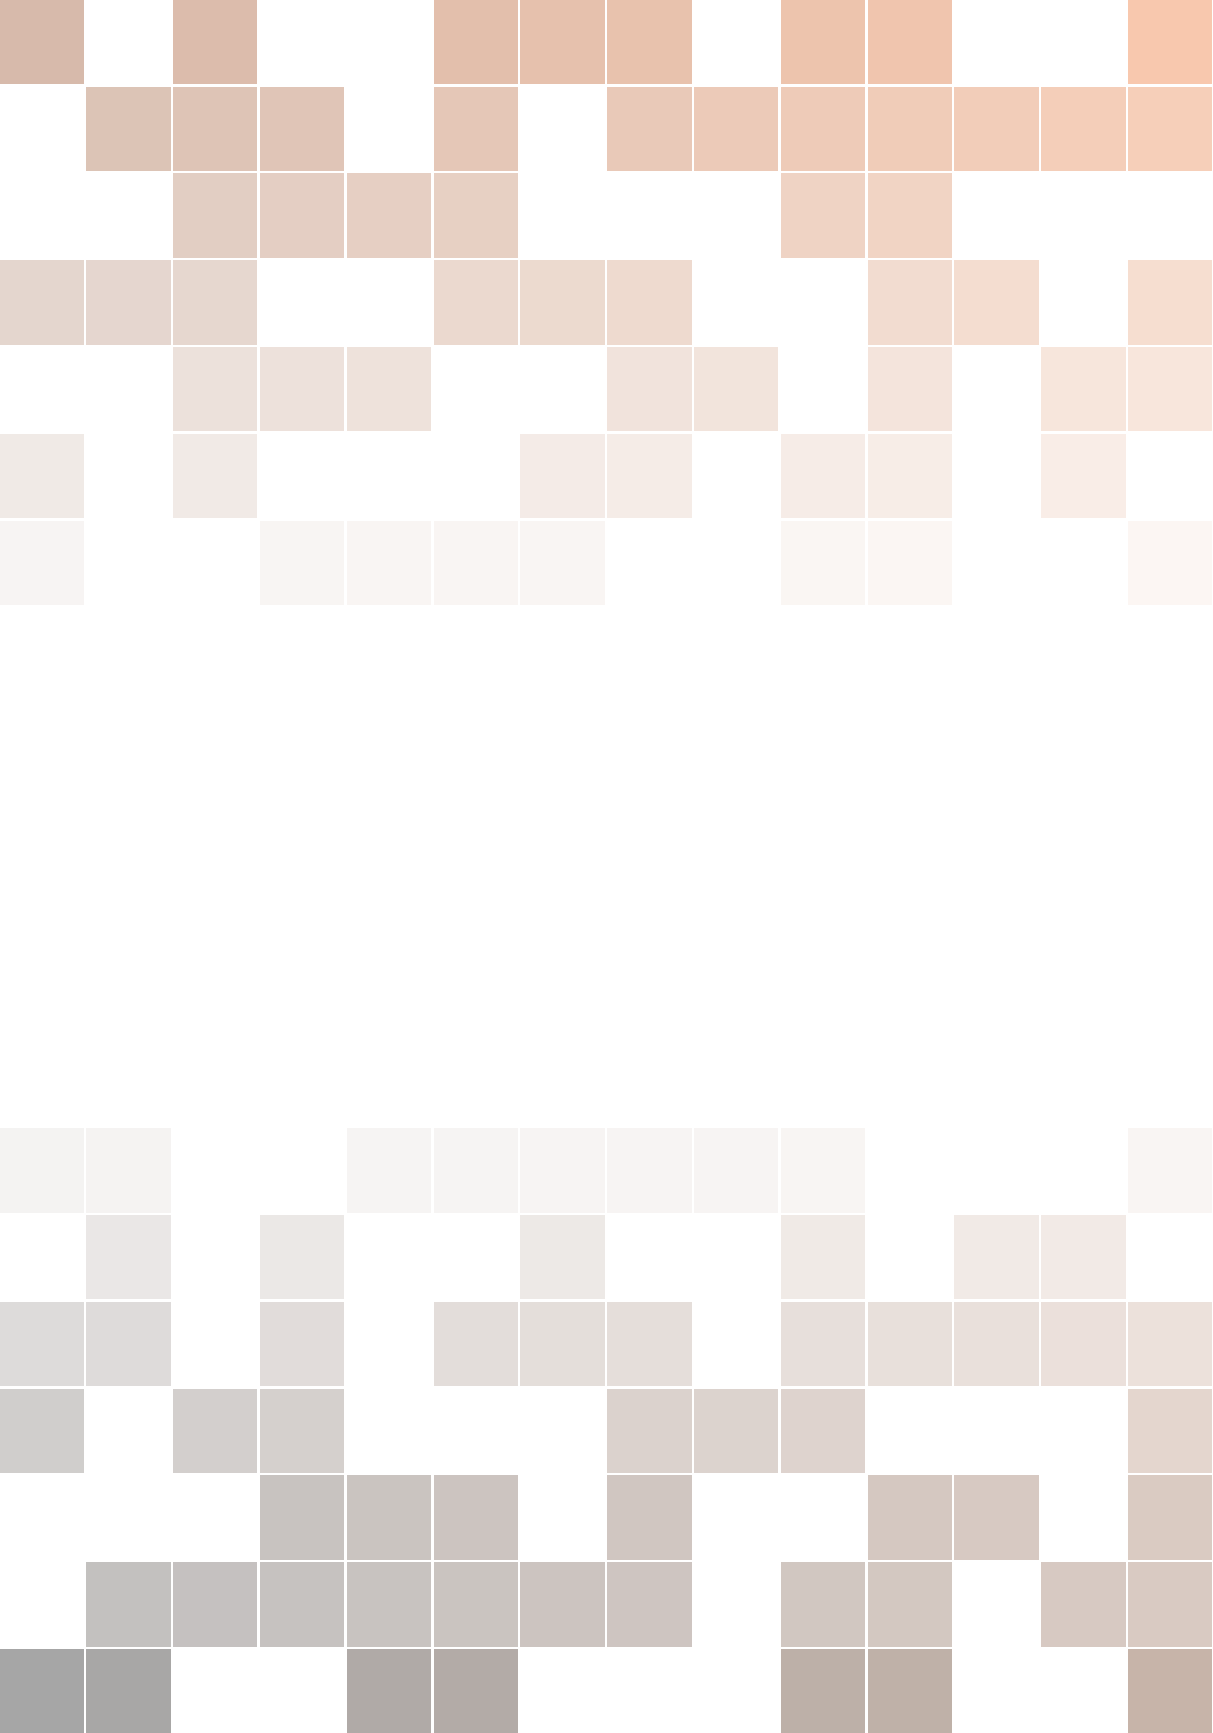
\includegraphics[scale=1]{background}}} % Image background
\par\normalfont\fontsize{15}{15}\sffamily\selectfont
“OpenQuake: Calculate, share, explore”
\centering
\vspace*{9cm}
\par\normalfont\fontsize{35}{35}\sffamily\selectfont
The OpenQuake-engine Book: Hazard\par % Book title
\endgroup

%----------------------------------------------------------------------------------------
%	COPYRIGHT PAGE
%----------------------------------------------------------------------------------------

\newpage
~\vfill
\thispagestyle{empty}

\noindent Copyright \copyright\ 2014 GEM Foundation\\ % Copyright notice

\noindent \textsc{Published by GEM Foundation}\\ % Publisher

\noindent \textsc{globalquakemodel.org/openquake}\\ % URL

\noindent 
   {\bf{Disclaimer}} \hfill \\
   The OpenQuake Engine Book Hazard is distributed in 
   the hope that it will be useful, but without any warranty: without 
   even the implied warranty of merchantability or fitness for a 
   particular purpose. While every 
   precaution has been taken in the preparation of this document, in 
   no event shall the authors of the manual and the GEM Foundation be 
   liable to any party for direct, indirect, special, incidental, or 
   consequential damages, including lost profits, arising out of the 
   use of information contained in this document or from the use of 
   programs and source code that may accompany it, even if the authors 
   and GEM Foundation have been advised of the possibility of such damage. 
   The Book provided hereunder is on as "as is" basis, and the authors 
   and GEM Foundation have no obligations to provide maintenance, support,
   updates, enhancements, or modifications. 
   \hfill \\
   \todo{This needs to be updated or removed}
   The current version of the book has been revised only by members of 
   the GEM model facility and it must be considered a draft copy. 
   %
   \vspace{0.4cm} \hfill \\
   {\bf{License}} \hfill \\
   This Book is distributed under the Creative Common License 
   Attribution-NonCommercial-NoDerivs 3.0 Unported (CC BY-NC-ND 3.0) 
   (see link below). You can download this Book and share it with 
   others as long as you provide proper credit, but you cannot change 
   it in any way or use it commercially. 
   \hfill \\

\noindent \textit{First printing, May 2014} % Printing/edition date

%----------------------------------------------------------------------------------------
%	TABLE OF CONTENTS
%----------------------------------------------------------------------------------------

\chapterimage{chapter_head_1.pdf} % Table of contents heading image

\pagestyle{empty} % No headers

\tableofcontents % Print the table of contents itself

\cleardoublepage % Forces the first chapter to start on an odd page so it's on the right

\pagestyle{fancy} % Print headers again

%----------------------------------------------------------------------------------------
%	CHAPTER 1
%----------------------------------------------------------------------------------------
\chapterimage{chapter_head_2.pdf} % Chapter heading image
\chapter{Introduction}
This chapter provides an overview of the \gls{acr:oqe}, 
its structure and the processes adopted for its development. 
A particular emphasis is placed on transparency, reproducibility,
community-based development and testing \parencite{pagani2014}, 
tenets endorsed since the early stages of development. 
%
% ..............................................................................
\section{Overview of the OpenQuake-engine}
%
The \gls{acr:oqe} is an open-source hazard and risk calculation engine 
whose development is actively supported by the 
\href{http://globalquakemodel.org}{\gls{acr:gem}} initiative.
%
The \gls{acr:oqe} is part of a suite of open-source software developed by 
\href{http://globalquakemodel.org}{\gls{acr:gem}} which comprises
(see also Figure \ref{fig:oq_platform}): 
the \gls{acr:oqe}, the OpenQuake-platform and a large set of tools of which 
the most interesting from a hazard perspective are the hazard modellers' 
toolkit (see \href{https://github.com/GEMScienceTools/hmtk}
{https://github.com/GEMScienceTools/hmtk}).

The development of the engine - started in 2010 and currently in 
progress - follows classical standards adopted for the development 
of open-source software such as open access of the source code though an easily
accessible website and transparency of the development process\footnote{See for 
example the documentation available on the website 
of the \href{http://opensource.org/osr}{Open-Source Initiative for a 
more comprehensive description of the development standards commonly 
adopted within the open-source software community}}.
The engine was designed to operate on hardware with different properties
ranging from a simple laptop to a heterogeneous cluster of multi-core machines.
The operative system currently supported is Ubuntu Linux (additional
information on the supported version and on the installation procedure can 
be found on the GEM area on github, accessible at the following link:
\href{https://github.com/gem/oq-engine}{https://github.com/gem/oq-engine}). 
% . . . . . . . . . . . . . . . . . . . . . . . . . . . . . . . . . . . > Figure
\begin{figure}[!ht]
\centering
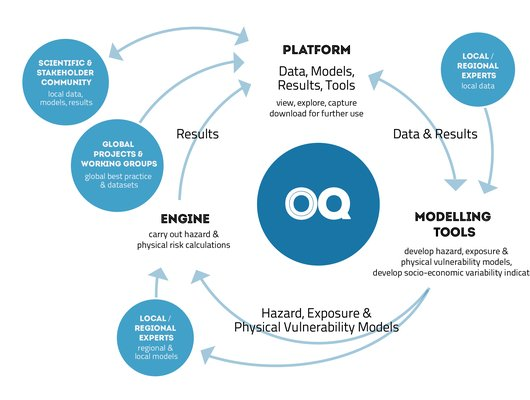
\includegraphics[width=14cm]{./Pictures/intro/OQ-workflows.jpg}
\caption{A schematic describing the OpenQuake suite.}
\label{fig:oq_platform}
\end{figure}
% . . . . . . . . . . . . . . . . . . . . . . . . . . . . . . . . . . . < Figure
%
% . . . . . . . . . . . . . . . . . . . . . . . . . . . . . . . . . . . . . . .
\subsection{Structure of the OpenQuake-engine}
The \gls{acr:oqe} is the combination of different and sometimes 
self-sufficient libraries. Below we provide a short description for each of
them.
\begin{description}
    \item [oq-hazardlib] Contains the code used to describe 
        seismic sources, create the \gls{acr:erf}, calculate hazard curves, 
        create stochastic event sets, compute ground motion fields and 
        calculate seismic hazard disaggregation.
    \item [oq-risklib] Comprises the code used to describe exposures, 
        vulnerability and fragility curves and to compute losses.
    \item [oq-nrmllib] Includes the scheme describing the structure of 
        the \gls{acr:oqe} input and output files. The majority of these files 
        is formatted according to a dialect of 
        \href{http://www.w3.org/XML/}{XML} called \gls{acr:nrml}. 
    \item [oq-commonlib] Includes common code for \gls{acr:oqe} applications,
        such as - for example - the code used to describe logic tree structures.
    \item [oq-engine] It incorporates the core of the \gls{acr:oqe}; 
        the code in this library acts as the glue that sticks the 
        different libraries together and lets the user easily perform 
        calculations according to an established set of calculation 
        options.
\end{description}
%
% ..............................................................................
\section{Overview of the OpenQuake-engine development process}
%
The \gls{acr:oqe} is developed through a close and continuous collaboration 
between the GEM scientific and IT teams. The development process is completely
carried out in the open in order to favor and promote the
participation of experts working in organizations different from the GEM 
Foundation.
%
% . . . . . . . . . . . . . . . . . . . . . . . . . . . . . . . . . . . . . . .
\subsection{Development tools}
%
The \gls{acr:oqe} development process is based on a number of open-source
tool which guarantee an open and transparent process. 
%
For example, each new feature improvement or bug fix before being 
implemented is described in a bug tracking system (in our case, 
\href{https://launchpad.net/}{Launchpad}).  

The tools used to maintain and make publicly available the \gls{acr:oqe} 
repository and to manage the almost ceaseless improvement and enhancement 
process are \href{http://git-scm.com/}{git} and a git-based repository 
hosting service called \href{http://github.com/}{GitHub}.
%
\begin{table}[!t]
\centering
\begin{tabular}{p{4cm}p{9cm}}
\hline
\rowcolor{anti-flashwhite}
\bf{Service} & \bf{Link}  \\
\hline 
OQ-engine main website & 
    \href{http://www.globalquakemodel.org/openquake/start/engine/}
        {http://www.globalquakemodel.org/openquake/start/engine/} \\
OQ-engine bug tracking system & 
    \href{https://launchpad.net/openquake}{https://launchpad.net/openquake} \\
OQ-engine web repository & 
    \href{http://github.com/gem}{http://github.com/gem} \\
\hline
\end{tabular}
\label{tab:development_tools}
\caption{Main services and websites related to the \gls{acr:oqe}}
\end{table}
Table \ref{tab:development_tools} provides a short summary of the main 
resources related to the \gls{acr:oqe}.
%
% . . . . . . . . . . . . . . . . . . . . . . . . . . . . . . . . . . . . . . .
\subsection{Programming language}
The core of the \gls{acr:oqe} is developed in 
\href{https://www.python.org/}{Python}. Python is a high level and open-source
programming language extensively used in the scientific community 
which can run on almost all the operative systems currently available.
%
% . . . . . . . . . . . . . . . . . . . . . . . . . . . . . . . . . . . . . . .
\subsubsection{Main libraries to which the \gls{acr:oqe} depends upon}
The engine relies in on a number of open-source libraries such as:
\begin{description}
    \item [\href{http://redis.io/}{Redis}] A key-value store
    \item [\href{https://www.rabbitmq.com/}{RabbitMQ}] A messaging system
    \item [\href{http://www.celeryproject.org/}{Celery}] An asynchronous 
        task queue/job queue.
\end{description}
%
% ..............................................................................
\section{The basics of the OpenQuake-engine hazard component}
%
The hazard component of the \gls{acr:oqe} has been developed mostly following 
an object oriented programming paradigm taking in some cases as an example 
concepts introduced in the development of OpenSHA, a seismic hazard 
analysis library developed within a joint SCEC-USGS collaboration 
\parencite{field2003}. 

From a conceptual point of view, the main objects adopted in the development
of the oq-hazardlib follows quite closely the classical schematic proposed by
\textcite{reiter1991} i.e. a seismic source, a ground shaking intensity model 
and a calculator that using this information computes the hazard at the site.

The \gls{acr:oqe} builds on top of oq-hazardlib and expands this 
concept by taking into account not just the essential objects 
needed to compute the hazard at a site discussed before but 
also the associated epistemic uncertainties.
%
% . . . . . . . . . . . . . . . . . . . . . . . . . . . . . . . . . . . . . . .
\subsection{Calculation workflows}
The hazard component of the \gls{acr:oqe} provides four main calculation 
workflows:
\begin{itemize}
\item Classical \gls{acr:psha}. Calculates hazard curves, hazard maps, 
    and uniform hazard spectra by solving the PSHA integration procedure, 
    as proposed by \textcite{field2003}. 
    This is the usual approach adopted in regional/national-scale hazard 
    assessment, as well as in site-specific studies. Using the risk 
    component of the OQ-engine, the computed hazard curves can be 
    combined with a vulnerability and exposure model to derive 
    asset-specific loss exceedance curves and loss maps for various 
    return periods. Such analyses are useful for comparative risk 
    assessment between assets at different locations, or to understand
    the areas where mitigation actions should be concentrated. 
    Crowley and Bommer (2006) suggest this methodology tends to 
    overestimate losses at high return periods for portfolios of 
    structures and recommend the use of methods capable to account 
    for the spatial correlation of ground motion residuals.
\item Event-based \gls{acr:psha}. Computes stochastic event sets (i.e., 
    synthetic catalogs of earthquake ruptures) and ground-motion fields 
    for each rupture, possibly taking into account the spatial 
    correlation of within-event residuals. This is essentially a 
    Monte Carlo–based PSHA calculator \parencite{musson2000}. The computed 
    synthetic catalogs can be used for comparisons against a real 
    catalog, whereas hazard curves and hazard maps can be derived from 
    post- processing the ground-motion fields \parencite{ebel1999}. 
    Ground-motion fields are essential input for loss estimations, 
    whereby loss exceedance curves and loss maps are calculated for 
    a collection of assets by combining a vulnerability and exposure
    model with these sets of ground- motion fields. Because the spatial
    correlation of the ground-motion residuals can be taken into account
    in this calculator, the losses to each asset can be summed per 
    ground-motion field, and a total loss exceedance curve representative 
    of the whole collection of assets can be derived. These results are 
    important for deriving reliable estimates of the variance of the
    total losses.
\item Scenario-based \gls{acr:sha}. Given an earthquake rupture and a 
    ground-shaking model, a set of ground-motion fields can be computed. 
    This is a typical use case for urban-scale loss analysis. This set of
    ground-motion fields can be em- ployed with a fragility/vulnerability 
    model to calculate distribution of damage/losses for a collection of
    assets. Such results are of importance for emergency management planning
    and for raising societal awareness of risk.
\item Disaggregation. Given a PSHA model, it computes the earthquake
    scenarios contributing the most to a given hazard level at a specific
    site \parencite{bazzurro1999}. Currently this is done following 
    the classical PSHA methodology; this functionality will be added to 
    the event-based calculator in subsequent development phases.
\end{itemize}
%
% . . . . . . . . . . . . . . . . . . . . . . . . . . . . . . . . . . . . . . .
\subsection{Testing and Quality Assurance}
%
Quality Assurance is an aspect carefully and diligently considered 
in the development of the \gls{acr:oqe}. There are a several 
different reasons explaining the adoption of this approach.

The first and most practical one is dictated by the development 
process which involves experts from different disciplines (e.g. 
seismic hazard and information technology). 
%
In this context the use of a formal testing process is a way 
trough which developers confirm the compliance of the tools 
developed against the requirements defined by the scientific 
team and it is also a process through which it can be 
demonstrated that the entire code fulfills minimum quality 
criteria (e.g. the code comply with the
\href{http://legacy.python.org/dev/peps/pep-0008/}{PEP 8 standard}, 
the code before getting into the master repository is 
revised by at least one one separate developer and is 
clearly documented).
 
The second motivation relates to the specific goal of building 
a dynamical tool (i.e. offering a large flexibility and expandability) 
while constantly assuring the stability and reliability of 
the supported calculation workflows.

The implementation of tests is usually done in parallel with code 
development, but tests are also added for example every time a bug 
is fixed.
%
This improves the overall robustness and reliability of the code
and reduces drastically the possibility of regressions.

Four are the approaches used to test the \gls{acr:oqe} behavior 
and therefore provide high quality assurance standards. 
%
\begin{description}
    \item [Unit-testing] A testing methodology which checks discrete 
        units of code against associated control data, expected behaviors 
        and operating procedures. A special set of unit-tests are the ones
        systematically created for every \gls{acr:gsim} implemented 
        (additional information about this specific topic is available within 
        Chapter \ref{chap:gmpes})
    \item [Testing against benchmark results] The results provided by the 
        \gls{acr:oqe} are compared benchmark results. Several of the 
        tests defined by \textcite{thomas2010} are used to check the 
        reliability and correctness of the results provided. 
    \item [Tests against provided by other PSHA codes: simple cases] 
        The result computed with the \gls{acr:oqe} for simple models (e.g. one
        area source) are compared against the results calculated using 
        independent PSHA software.
    \item [Tests against provided by other PSHA codes: national or regional 
        PSHA input models] \hfill \\ The result computed with the \gls{acr:oqe} 
        using national or regional models are compared against the 
        results calculated using independent PSHA software.
\end{description}
%
% ..............................................................................
\section{Input and output description}
This part will be completed later.
%
% ..............................................................................
\section{Description of book structure}
This part will be completed later.


%----------------------------------------------------------------------------------------
%	CHAPTER 2
%----------------------------------------------------------------------------------------
\chapterimage{chapter_head_2.pdf} % Chapter heading image
\chapter{PSHA with the OpenQuake-engine}
This chapter describes the mathematical framework for PSHA implemented by the OpenQuake-engine.
Seismicity is assumed to be described as a time-indipendent Poissonian process. Seismicity modeling
relies therefore on the following three assumptions:
\begin{itemize}
	\item seismicity in a region is described by a collection of \textit{indipendent seismic sources}
	(i.e. the occurrence of an earthquake rupture in a source does not affect the probability of
	earthquake occurrence in the other sources)
	\item each source generates \textit{indipendent earthquake ruptures} (i.e. the occurrence of an
	earthquake rupture in a source does not affect the probability of occurrence of the other
	potential earthquake ruptures in the same source)
	\item the number of occurrences for each earthquake rupture in a source follows a \textit{Poissonian}
	distribution
\end{itemize}

\section{Basic concepts}
The Classical, Event-Based, and Disaggregation analysis requires the definition of two main components:
the \textit{seismic source model}, that is a collection of seismic sources describing the seismic activity in a
region of interest, and the \textit{ground motion model}, that is a mathematical relationship defining the
probability distribution of a ground motion parameter at a site given the occurrence of an earthquake
rupture.\\
The design of a seismic source model involves the specification of a number of sources whose main parameters
are the geometry, constraining the earthquake rupture locations, and the \textit{magnitude-frequency
distribution}, defining the average annual occurrence rate over a magnitude range. Chapter \ref{chap:ssm} provides
a detailed description of the different source typologies supported by the OQ-engine. However, indipendently
of the typology, in a PSHA each source undergoes a discretization process which effectively generates a
number of distinct earthquake ruptures. We can therefore assume a source to define a set of earthquake ruptures:
\begin{equation}
Src = \left\{Rup_{1}, Rup_{2}, ..., Rup_{J}\right\}
\end{equation}
By indicating with $\nu_{j}$ the average annual occurrence rate for the $j-th$ rupture, the probability of the
$j-th$ rupture to occur $k$ times in a time span $T$ can be written, accordingly with the Poissonian assumption,
as:
\begin{equation}
\label{eq:poisson_pd}
P_{rup_{j}}(k | T) = e^{-\nu_{j} T} \frac{(\nu_{j} T) ^ {k}}{k!}
\end{equation}

\section{The hazard equation for \textit{Classical} PSHA}
The classical PSHA analysis allows calculating the probabilities of exceeding, at least once in a given time
span, and at a given site, a set of ground motion parameter levels considering all possible earthquake ruptures
defined in a seismic source model. Such a list of probability values is usually referred to as \textit{hazard curve}.
We indicate with $P(X \ge x | T)$ the probability that a ground-motion parameter $X$ exceeds, at least once in
a time span $T$, a level $x$. $P(X \ge x | T)$ can be computed as 1 minus the probability that none of the
sources is causing a ground motion exceedance. By assuming \textit{indipendent sources}, the probability
that none of the sources is causing an exceedance is equal to the product of the probabilities that each source
does not cause an exceedance, that is:
\begin{align}
\label{eq:hazard_eq}
P(X \ge x | T) & =  1 - P_{src1}(X < x | T) * P_{src2}(X < x | T) * ... * P_{srcI}(X < x | T) \nonumber \\
		      & =  1 - \prod_{i=1}^{I} P_{src_{i}}(X < x | T)
\end{align}
where $P_{src_{i}}(X < x | T)$ is the probability that the $i-th$ source is not causing an exceedance and $I$ is the
total number of sources in the source model. By further assuming each source generates \textit{indipendent
earthquake ruptures}, we can compute $P_{src_{i}}(X < x | T)$ as the product of the probabilities that each rupture
does not cause an exceedance, that is:
\begin{align}
\label{eq:prup_noexceed_src}
P_{src_{i}}(X < x | T) & = P_{rup_{1}}(X < x | T) * P_{rup_{2}}(X < x | T) * ... * P_{rup_{J}}(X < x | T) \nonumber \\
			        & = \prod_{j=1}^{J} P_{rup_{j}}(X < x | T)
\end{align}
where $P_{rup_{j}}(X < x | T)$ is the probability that the $j-th$ rupture is not causing an exceedance and $J$ is
the total number of ruptures generated by the source. Intuitively, the fact that a rupture does not cause any
exceedance in a given time span T can be due to the fact that the rupture does not occur at all or that the
rupture occurs once but without causing an exceedance, or that the rupture occurs twice but both times
without causing an exceedance, and so on. Given that all these events are mutually exclusive, by using the
total probability theorem we can write:
\begin{align}
\label{eq:prup_noexceed_rup}
P_{rup_{j}}(X < x | T) & = P_{rup_{j}}(n = 0 | T) + P_{rup_{j}}(n = 1 | T) * P(X < x | rup_{j}) + \nonumber \\
                                &\quad	P_{rup_{j}}(n = 2 | T) * P(X < x | rup_{j})^{2}  + ... \nonumber \\
				 & = \sum_{k=0}^{\infty} P_{rup_{j}}(k | T) * P(X < x | rup_{j}) ^ {k} 
\end{align}
where $P_{rup_{j}}(k | T)$ is the probability that the $j-th$ rupture is occurring $k$ times in time span $T$ and
$P(X < x | rup_{j})$ is the conditional probability that parameter $X$ is not exceeding level $x$ given an
occurrence of the $j-th$ rupture.\\
By now assuming that the \textit{number of occurrences of each rupture in a time span $T$ follows a Poissonian distribution}
we can place equation \ref{eq:poisson_pd} in \ref{eq:prup_noexceed_rup} and thus write:
\begin{align}
\label{eq:prup_noexceed_rup_pois_v0}
P_{rup_{j}}(X < x | T) & = \sum_{k=0}^{\infty} e^{-\nu_{j} T} \frac{(\nu_{j} T) ^ {k}}{k!} * P(X < x | rup_{j}) ^ {k} \nonumber \\
				 & =  e^{-\nu_{j} T} \sum_{k=0}^{\infty} \frac{(\nu_{j} T * P(X < x | rup_{j})) ^ {k}}{k!}
\end{align}
Making use of the property:
\begin{equation}
e^{x} = \sum_{k=0} ^ {\infty} \frac{x^{k}}{k!}
\end{equation}
we can rewrite \ref{eq:prup_noexceed_rup_pois_v0} as:
\begin{align}
\label{eq:prup_noexceed_rup_pois_v1}
P_{rup_{j}}(X < x | T) & = e^{-\nu_{j} T} e ^ {\nu_{j} T * P(X < x | rup_{j})} \nonumber \\
				 & = e^{-\nu_{j} T * (1 - P(X < x | rup_{j}))} \nonumber \\
				 & = e^{-\nu_{j} T * P(X \ge x | rup_{j})}
\end{align}
By now recognizing that, according to the Poissonian distribution, the probability of at least one occurrence
(that is one or more) in a time span $T$ of the $j-th$ rupture can be written as:
\begin{equation}
P_{rup_{j}}(n \ge 1 | T) = 1 -  e^{-\nu_{j} T}
\end{equation}
we can write equation \ref{eq:prup_noexceed_rup_pois_v1} as:
\begin{equation}
\label{eq:prup_noexceed_rup_pois_v2}
P_{rup_{j}}(X < x | T) = (1 - P_{rup_{j}}(n \ge 1 | T))^{P(X \ge x | rup_{j})}
\end{equation}
By placing equation \ref{eq:prup_noexceed_rup_pois_v2} in \ref{eq:prup_noexceed_src}, we can thus
write equation \ref{eq:hazard_eq} as:
\begin{equation}
\label{eq:hazard_eq_poiss}
P(X \ge x | T) =  1 - \prod_{i=1}^{I} \prod_{j=1}^{J} (1 - P_{rup_{j}}(n \ge 1 | T))^{P(X \ge x | rup_{j})}
\end{equation}
Equation \ref{eq:hazard_eq_poiss} is used by the OQ-engine for the calculation of hazard curves when performing
\textit{Classical} PSHA. To our knowledge, this equation has been first proposed by \cite{field2003},
derived from the traditional rate-based formulation converted in terms of probabilities (their equation A8).
Instead, we derive it from the assumptions of a source model consisting of independent sources, independent
earthquake ruptures generated by each source, and ruptures obeying to a Poissonian temporal occurrence model.

\subsection{Equivalence with the rate-based equation}
It is worth noticing how equation \ref{eq:hazard_eq_poiss} is equivalent to the more traditional rate-based
hazard equation (\cite{mcguire1995}). Indeed, by assuming ground motion occurrence to follow a Poissonian
distribution in time, and indicating with $\nu$ the mean annual rate of exceeding a ground motion level x,
we can write:
\begin{equation}
\label{eq:hazard_eq_rate}
P(X \ge x | T) = 1 - e ^ {- \nu T}
\end{equation}
We can also rewrite \ref{eq:hazard_eq_poiss} as:
\begin{align}
\label{eq:hazard_eq_prob}
P(X \ge x | T) &= 1 - \prod_{i=1}^{I} \prod_{j=1}^{J} (1 - P_{rup_{j}}(n \ge 1 | T))^{P(X \ge x | rup_{j})} \nonumber \\
		      &= 1 - \prod_{i=1}^{I} \prod_{j=1}^{J} e^{-\nu_{j} T * P(X \ge x | rup_{j})} \nonumber \\
		      & = 1 - e ^ {- \sum_{i=1}^{I} \sum_{j=1}^{J} \nu_{j} T * P(X \ge x | rup_{j})}
\end{align}
The equivalence between equations \ref{eq:hazard_eq_rate} and \ref{eq:hazard_eq_prob} is possible if and only if:
\begin{align}
\label{eq:equivalence_condition_0}
\nu  =  \sum_{i=1}^{I} \sum_{j=1}^{J} \nu_{j} * P(X \ge x | rup_{j})
\end{align}
Assuming now, for the sake of simplicity, that a rupture is completely characterized by magnitude and distance from a site, we
can write the rate of occurrence of the $j-th$ rupture as:
\begin{equation}
\label{eq:rup_rate}
\nu_{j} = \nu_{i} * f_{i}(m, r)
\end{equation}
where $\nu_{i}$ is the total occurrence rate for the $i-th$ source, and $f_{i}(m, r)$ is the probability, for the $i-th$ source, of
generating a rupture of magnitude $m$ and distance $r$. By placing \ref{eq:rup_rate} in \ref{eq:equivalence_condition_0} and
by replacing the discrete summation over ruptures with a continuous integral over magnitude and distance, we can write:
\begin{align}
\nu = \sum_{i=1}^{I} \nu_{i} \iint f_{i}(m, r) P(X \ge x | m, r)\,dm \,dr
\end{align}
which is the traditional equation for calculating ground motion exceedance rates (CITE MCGUIRE 1995).

\section{Generation of stochastic event sets and ground motion fields for \textit{Event-based} PSHA}
The goal of an \textit{Event-based} PSHA is to simulate seismicity in a region as described by a source model
and to simulate ground shaking on a set of locations accordingly with a ground motion model. In both
cases, simulation invoves on a Monte Carlo (i.e. random) sampling procedure.\\
Seismicity is simulated by generating a \textit{stochastic event set} (also known as \textit{synthetic catalog})
for a given time span $T$. For each source in a source model, and for each rupture generated by a source,
the number of occurrences in a time span $T$ is simulated by sampling the corresponding probability
distribution as given in equation \ref{eq:poisson_pd}. A stochastic event set is therefore a \textit{sample}
of the full population of ruptures as defined by a seismic source model. Each rupture is present zero, one or
more times, depending on its probability. Symbolically, we can define a stochastic event ($SES$) set as:
\begin{align}
SES(T) = \left\{k \times rup,\;k\sim P_{rup}(k | T)\;\;\forall\;rup\;in\;Src\;\forall\;Src\;in\;Source\;Model\right\}
\end{align}
where $k$, the number of occurrences, is a random sample of $P_{rup}(k | T)$, and $k \times rup$ means
that rupture $rup$ is repeated $k$ times in the stochastic event set.

Given an earthquake rupture, the simulation of ground shaking values on a set of locations ($\bm{x}=(x_{1}, x_{2}, ..., x_{N})$)
forms a \textit{ground motion field}. In a \textit{Event-based} PSHA, for each rupture in a stochastic event set,
the ground motion field is obtained by sampling the probability distribution defined by the ground motion model.
As described in Chapter \ref{chap:gmpes}, the ground motion distribution at a site is assumed to be a Normal
distribution. The aleatory variability is described in terms of an \textit{inter-event} (also known as \textit{between-events})
standard deviation ($\tau$) and \text{intra-event} (also known as \textit{within-event}) standard deviation ($\sigma$).
The simulation of a ground motion field is therefore the result of the summation of three terms, the mean of the
ground motion distribution:
\begin{equation}
\bm\mu = (\mu_{1}, \mu_{2}, ..., \mu_{N})
\end{equation}
the inter-event variability:
\begin{equation}
\bm\eta = (\eta, \eta, ..., \eta),\;where\;\eta\sim N(0, \tau)
\end{equation}
and the intra-event variability:
\begin{align}
\bm\epsilon = (\epsilon_{1}, \epsilon_{2}, ..., \epsilon_{N}) \sim N(\bm{0}, \bm\Sigma)
\end{align}
where:
\begin{align}
\bm\Sigma = 
\begin{bmatrix}
\sigma_{1}^2&\sigma_{1}\sigma_{2}\rho_{12}&\cdots &\sigma_{1}\sigma_{N}\rho_{1N} \\
\sigma_{2}\sigma_{1}\rho_{21}&\sigma_{2}^2&\cdots &\sigma_{2}\sigma_{N}\rho_{2N} \\
\vdots & \vdots & \ddots & \vdots\\
\sigma_{N}\sigma_{1}\rho_{N1}&\sigma_{N}\sigma_{2}\rho_{N2}&\cdots &\sigma_{N}^2
\end{bmatrix}
\end{align}
It is worth noticing how the inter-event variability, uniform for all sites given an earthquake rupture, is drawn
from an univariate normal distribution of mean 0 and standard deviation $\tau$, while the intra-event variability
is a random sample of a multivariate normal distribution of mean $\bm{0}$ and covariance matrix $\bm\Sigma$.
$\bm\Sigma$ is a diagonal matrix when considering no-correlation in the intra-event variability, while has non-zero
off-diagonal elements when considering a correlation model for the intra-event aleatory variability.

\subsection{Calculation of hazard curves from ground motion fields}
The ground motion fields simulated for each rupture in a stochastic event set can be used to
compute hazard curves. Indeed, indicating with $T_{0}$ the duration associated with a stochastic
event set, and with $K$ the number of ground motion fields (and associated ruptures) simulated
in time $T_{0}$, we can compute the rate of exceedance of a ground motion level $x$ at a site as (\cite{ebel1999}):
\begin{align}
\label{eq:rate_from_gmfs}
\nu = \frac{\sum_{k=1}^{K}H(x_{k} - x)}{T_{0}}
\end{align}
where $H$ is the Heaviside function and $x_{k}$ is the ground motion parameter value at the considered site associated
with the $k-th$ ground motion field. The exceedance rate obtained from equation \ref{eq:rate_from_gmfs} can then be
used to compute the probability of at least one occurrence in any time span $T$, accordingly with the Poissonian distribution,
using equation \ref{eq:hazard_eq_rate}.\\
As the stochastic event set duration $T_{0}$ increases, equation \ref{eq:rate_from_gmfs}
provides an increasingly more accurrate estimate of the actual rate of exceedance. A larger $T_{0}$ can be achieved
not only by simulating a single stochastic event set with longer duration, but also by simulating multiple
stochastic event sets. These can then be joined together to form a stochastic event which has a large enough
duration to provide a stable estimate of the rates of ground motion exceedance.

\section{Disaggregation analysis}
The disaggregation analysis allows investigating how the different earthquake ruptures defined in a source model
contribute to the probability of exceeding a certain ground motion level $x$ at a given site. Given the very
large number of earthquake ruptures associated with a source model, contributions cannot be investigated on a rupture by
rupture basis but a classification scheme is used instead. Ruptures are classified in terms of the following parameters:
\begin{itemize}
	\item magnitude ($M$)
	\item distance to rupture surface-projection (Joyner-Boore distance) ($r_{jb}$)
	\item longitude and latitude of rupture surface-projection closest point ($\lambda$, $\phi$)
	\item tectonic region type ($TRT$)
\end{itemize}
For each earthquake rupture, the associated conditional probability of exceedance - $P(X \ge x | T, rup)$ - is computed
for different $\epsilon$ bins, where $\epsilon$ is the difference, in terms of number of total standar deviations,
between $x$ and the mean ground motion $\mu$ as predicted by the ground motion model, that is:
\begin{equation}
\epsilon = \frac{x - \mu}{\sigma_{total}}
\end{equation}
The disaggregation in terms of $\epsilon$ allows investigating what are the regions of the ground motion distributions
that are contributing the most to the probability of exceedance.\\
The rupture parameters ($M$, $r_{jb}$, $\lambda$, $\phi$, $TRT$) together with the $\epsilon$ parameter effectively
create a 6-dimensional model space which, discretized into a number of bins, is used to classify the probability
of exceedance for different combination of rupture parameters and $\epsilon$ values.\\
For a given model space bin $\bm{m} = (M, r_{jb}, \lambda, \phi, TRT, \epsilon)$ the probability of
exceeding level $x$ at least once in a time span $T$ is computed using equation \ref{eq:hazard_eq_poiss}, that is:
\begin{align}
\label{eq:disagg}
P(X > x | T, \bm{m}) =
	1 - \prod_{i=1}^{I}\prod_{j=1}^{J}
	\begin{cases} (1 - P_{rup_{j}}(n \ge 1 | T))^{P(X \ge x | rup_{j}, \epsilon)} & \mbox{if}\;rup_{j}\;\in\;\bm{m}\\
			      1 & \mbox{if}\;rup_{j}\;\notin\;\bm{m}
	\end{cases}
\end{align}

\subsection{Disaggregation histograms}
Disaggregation values as given by equation \ref{eq:disagg} can be aggregated in order to investigate earthquake rupture
contributions over a reduced model space.\\
Magnitude disaggregation can be obtained as:
\begin{equation}
P(X > x | T, M) = 1 -\prod_{r_{jb}}\prod_{\lambda}\prod_{\phi}\prod_{TRT} \prod_{\epsilon}(1 - P(X > x | T, \bm{m}))
\end{equation}
Distance disaggregation:
\begin{equation}
P(X > x | T, r_{jb}) = 1 -\prod_{M}\prod_{\lambda}\prod_{\phi}\prod_{TRT} \prod_{\epsilon}(1 - P(X > x | T, \bm{m}))
\end{equation}
Tectonic region type disaggregation:
\begin{equation}
P(X > x | T, TRT) = 1 -\prod_{M}\prod_{r_{jb}}\prod_{\lambda}\prod_{\phi} \prod_{\epsilon}(1 - P(X > x | T, \bm{m}))
\end{equation}
Magnitude-Distance disaggregation:
\begin{equation}
P(X > x | T, M, r_{jb}) = 1 -\prod_{\lambda}\prod_{\phi}\prod_{TRT}\prod_{\epsilon}(1 - P(X > x | T, \bm{m}))
\end{equation}
Magnitude-Distance-Epsilon disaggregation:
\begin{equation}
P(X > x | T, M, r_{jb}, \epsilon) = 1 -\prod_{\lambda}\prod_{\phi}\prod_{TRT}(1 - P(X > x | T, \bm{m}))
\end{equation}
Longitude-Latitude disaggregation:
\begin{equation}
P(X > x | T, \lambda, \phi) = 1 -\prod_{M}\prod_{r_{jb}}\prod_{TRT}\prod_{\epsilon}(1 - P(X > x | T, \bm{m}))
\end{equation}
Longitude-Latitude-Magnitude disaggregation:
\begin{equation}
P(X > x | T, \lambda, \phi, M) = 1 -\prod_{r_{jb}}\prod_{TRT}\prod_{\epsilon}(1 - P(X > x | T, \bm{m}))
\end{equation}
Longitude-Latitude-Tectonic Region Type disaggregation:
\begin{equation}
P(X > x | T, \lambda, \phi, TRT) = 1 -\prod_{M}\prod_{r_{jb}}\prod_{\epsilon}(1 - P(X > x | T, \bm{m}))
\end{equation}

%This chapter contains a general introduction to \gls{acr:sha} and a 
%description of the main concepts needed to understand the hazard calculation 
%methodologies implemented in the OpenQuake-engine.

%\Gls{psha} is a methodology to compute the probability that ground motion, 
%for a site or region, will exceed a given level of intensity in a specified 
%time period. Originally formulated in the classic works of \cite{cornell1968} 
%and \cite{esteva1968}, the fundamental theory of \gls{acr:psha} has remained 
%robust. 
%Over the last four decades there have been many developments that have 
%increased 
%the accuracy and rigour of the process, particularly with respect to the 
%treatment of uncertainties.
%
% ..............................................................................
%\section{Common concepts}
%
%\subsection{Magnitude-frequency distributions}
%\index{Magnitude-frequency distribution}
%
%In statistics a distribution represents an arrangment of the 

%The OpenQuake-engine supports the following \glspl{acr:mfd}:
%\begin{itemize}
%   \item Double-truncated Gutenberg-Richter;
%  \item Evenly-spaced;
%    \item Characteristic \cite{youngs1985}
%\end{itemize}
%
% . . . . . . . . . . . . . . . . . . . . . . . . . . . . . . . . . . . . . . .
%\subsection{Magnitude-scaling relationships}
%
%\glspl{acr:msr} - a fundamental component of a seismic hazard analysis - are 
%empirical functions linking independent an independent variable (e.g. 
%magnitude) to a parameter describing some properties of the earthquake 
%rupture geometry (e.g. area or length).
%
% . . . . . . . . . . . . . . . . . . . . . . . . . . . . . . . . . . . . . . .
%\subsection{Ground-motion prediction equations}
%\index{Ground-motion prediction equation}
%A \gls{acr:gmpe} is an empirical relationship which associates a number of 
%predictive 
%
% . . . . . . . . . . . . . . . . . . . . . . . . . . . . . . . . . . . . . . .
%\subsection{Local soil conditions}
%
% ..............................................................................
%\section{Methodologies for seismic hazard analysis}
%\index{Seismic hazard analysis}
%The hazard integral as implemented in the \gls{acr:oqe}

%\cite{cornell1968}
%\cite{mcguire2004}
%
% . . . . . . . . . . . . . . . . . . . . . . . . . . . . . . . . . . . . . . .
%\subsection{Scenario-based Hazard Analysis}
%\index{Seismic hazard analysis!Scenario-based}
%
% . . . . . . . . . . . . . . . . . . . . . . . . . . . . . . . . . . . . . . .
%
%\subsection{Classical Probabilistic Seismic Hazard Analysis}
%\index{Seismic hazard analysis!Classical PSHA}
%
% . . . . . . . . . . . . . . . . . . . . . . . . . . . . . . . . . . . . . . .
%\subsection{Event-Based Probabilistic Seismic Hazard Analysis}
%\index{Seismic hazard analysis!Event-based PSHA}
%
% . . . . . . . . . . . . . . . . . . . . . . . . . . . . . . . . . . . . . . .
%\subsection{Disaggregation}
%\index{Seismic hazard analysis!Disaggregation}
%
% . . . . . . . . . . . . . . . . . . . . . . . . . . . . . . . . . . . . . . .
%\section{What's missing}
%\subsection{Vector based PSHA}
%\index{Seismic hazard analysis!Vector-based PSHA}
%\subsection{PFDHA}
%\index{Seismic hazard analysis!Probabilistic fault displacement hazard analysis}
%\subsection{PSHA using site-specific transfer functions}


%----------------------------------------------------------------------------------------
%	CHAPTER 4
%----------------------------------------------------------------------------------------
\chapterimage{chapter_head_1.pdf} % Chapter heading image
\chapter{Seismic Source Models}
\label{chap:ssm}
This chapter describes the seismic source typologies supported by the OQ-engine:
\textit{Point} and \textit{Area} sources for modeling distributed seismicity,
\textit{Simple Fault}, \textit{Complex Fault}, and \textit{Characteristic Fault}
for modeling fault-based seismcity.

\section{Basic concepts}
\index{Seismic source}
%------ The different source typologies ------%
%------ Point and Area ----------%
The OQ-engine provides several seismic source typologies to accomodate different
modeling approaches. For modeling distributed seismicity, that is seismic
activity occurring over a geographical region and not tied to specific well
characterized fault structures, the OQ-engine provides the \textit{Point} and
\textit{Area} sources. The former defines seismic activity \textit{nucleating in
a single geographical location}, while the second seismicity occurring
\textit{uniformly over a geographical region}. 
% 
Both sources define a seismogenic layer which constrains rupture location and
extension along depth. A collection of Point sources can be used to model
seismicity with spatially variable parameters (as obtained from a smoothed
seismicity approach for instance), while Area sources can be used to model
seismicity in geographic zones usually defined by expert judgments taking into
account seismological, geological and geodetic information. 
%
Both source typologies allow for the modeling of earthquake ruptures as extended
surfaces (that is as rectangular planes) with potentially multiple orientations
and inclinations (that is multiple strike and dip angles) and also placed at
different depth levels. Earthquake ruptures can extend without barriers along
strike but cannot cross the seismogenic layer.

%------- Faults ---------%
For modeling fault-based seismicity, that is seismic activity occurring on a
well identified and characterized fault zone, the OQ-engine provides three 
main options, the \textit{Simple Fault}, the \textit{Complex Fault} and
the \textit{Characteristic Fault} sources.

The Simple and Complex Faults distribute seismicity \textit{uniformly over a
fault surface}, with the only constraint that an earthquake rupture cannot
extend outside of the defined fault surface. In both sources an earthquake of a
given magnitude is defined as a portion of the fault surface. 
%
To simulate all possible rupture locations, an earthquake rupture is moved, or
\textit{floated}, over the entire fault surface. The two source typologies
differ instead in terms of the geometrical complexity they can accommodate when
modeling a fault surface. In particular, a Simple Fault source can model a fault
surface as a plain rectangle in the simplest case, or as a set of connected
parallelograms in the most complex case. 
%
A Complex Fault source can instead model an arbitrarily complex
quadrilateral surface, which can therefore accommodate changes in dip angle
along depth or along strike or changes in fault width. The Complex Fault source
is therefore particularly suitable for modeling large subdution interface
faults, while Simple Fault sources can be used for modeling crustal faults. 

The \textit{Characteristic Fault} source can model both simple and complex
geometries, but instead of simulating floating ruptures, each earthquake breaks
the entire fault surface independently of the associated magnitude. The
Characteristic Source typology can be used to model individual faults or fault
segments that tend to produce essentially same size earthquakes
(\cite{schwartscoppersmith1984}).

%-------- Common parameters -------%
%-------- Magnitude-Frequency Distribution-------%
Independently of the typology, all sources require the definition of the
following main parameters:
\begin{itemize}
\item magnitude-frequency distribution
\item temporal occurrence model
\item tectonic region type
\item magnitude-area scaling relationship (for all but the Characteristic Fault source)
\item rupture-aspect ratio (for all but the Characteristic Fault source)
\item upper seismogenic depth
\item lower seismogenic depth
\end{itemize}
%
\index{Magnitude-frequency distribution}
The magnitude-frequency distribution defines the total moment rate released by a
source as well as the relative frequency of earthquakes of different magnitude
that can be generated by this source. It is therefore a key object
controlling the influence of a source in a PSHA. 

The OQ-engine supports the definition of the traditional
\textit{double-truncated Gutenberg-Richter} magnitude-frequency distribution
which is widely used in PSHA. 
%
The parameters required for its definition are the \textit{a-value}
(defined as the intercept of the \textit{cumulative} distribution at $M=0$ in a
$log_{10}$ scale), the \textit{b-value}, the minimum and the maximum magnitudes.
%
In order to accommodate other possible parametric (and non-parametric) forms of
the magnitude-frequency distribution, the OQ-engine provides a generic discrete
\textit{Incremental} magnitude-frequency distribution defined through a list of
annual occurrence rates, associated to an equally spaced set of magnitude
values.
%
The OQ-hazardlib contains also a implementation of the \textcite{youngs1985}
magnitude-frequency distribution. This distribution is currently non available 
in the \gls{acr:oqe}. With future releases, we plan to make this distribution
available to the \gls{acr:oqe} users.

In a PSHA, the magnitude-frequency distribution is subject to a discretization
process which defines a set of equally spaced magnitude bins and the associated
annual occurrence rates (for an \textit{Incremental} magnitude-frequency
distribution such a discretization is part of its definition). For each source,
the annual occurrence rate associated to a magnitude bin is \textit{uniformly}
distributed over all the ruptures associated to the same magnitude bin value. In
other words, while the particular geometry of a source determines location and
number of ruptures of a given magnitude, the occurrence rate (and thus the
occurrence probability) is uniform over ruptures with the same magnitude.

%----------Temporal occurrence model---------%
The temporal occurrence model defines the functional form used to compute the probability of
the number of rupture occurrences in a given time span based on the occurrence rate specified
by the magnitude frequency distribution, that is the term $P_{rup_{ij}}(k | T)$ in equation
\ref{eq:hazard_eq_ind_srcs_rups}. Currently the \gls{acr:oqe} defines only the Poissonian model
(that is equation \ref{eq:poisson_pd}) but other functional forms can be introduced.

%----------Tectonic Region Type---------%
The tectonic region type is an attribute used as a key to associate a seismic source to a ground
motion model. Given a source model describing seismicity occurring in a region
including different tectonic settings, the associated ground motion model may
prescribe different equations for the different tectonic settings. The mapping
between a ground motion model equation and a seismic source is therefore
achieved through the tectonic region type attribute.

%-----------Magnitude-Area Scaling and Rupture Aspect Ratio----------%
\index{Magnitude-scaling relationship}
All sources typologies supported by the \gls{acr:oqe} generate ruptures as
extended surfaces. With the only exception of the Characteristic Fault source,
the area of an earthquake rupture surface is magnitude dependent. To constrain
the rupture surface area, the Point, Area, Simple and Complex Fault sources
require the definition of a \textit{magnitude-area} scaling relationship.
This parameter together with a \textit{rupture aspect ratio} (defined as ratio
between length and width) completely define the rupture extension and shape
(assumed rectangular). Indeed, indicating with $A$ the rupture area and with
$ar$ the rupture aspect ratio, rupture length ($L$) and and width ($W$) can be
computed as:
\begin{equation}
\begin{split} \label{eq:rup_l_w}
&L = \sqrt{A * ar}  \\
&W = \sqrt{A / ar}
\end{split}
\end{equation}
In all sources, the rupture aspect ratio is used to constrain the initial
rupture shape. However, if this conflicts with other source-dependent
geometrical constrains, the rupture is reshaped so as to conserve the area as
given by the scaling relationship.

%-----------Upper and Lower Seismogenic Depths-------------%
\index{Seismogenic depth!upper}
\index{Seismogenic depth!lower}
The upper and lower seismogenic depths define the seismogenic layer, that is the
depth range over which earthquake ruptures can extend. The definition of a
seismogenic layer is required to avoid an uncontrolled extension of the
earthquake ruptures along depth which can lead, especially for large magnitude
events, to unrealistic scenarios. The definition of a seismogenic layer
thickness effectively induces a magnitude-dependent rupture aspect ratio.
Indeed, as the rupture size increases with increasing magnitude values, the
rupture width reaches the maximum allowed width, and the rupture aspect ratio
starts deviating, that is increasing, from the original value.

\section{The Point and Area sources}
\index{Seismic source!Point}
\index{Seismic source!Area}
The parameters specific to the definition of Point and Area sources, and their
associated function, are listed in Table \ref{table:point_area_tab}.
\begin{table}
\centering
\caption{Table summarizing parameters, and their functions, required for the
definition of Area and Point sources in the OQ-engine}
\begin{tabular}{|p{60mm} p{60mm}|}
\hline
\rowcolor{anti-flashwhite}
\bf{Parameter} & \bf{Purpose} \\ \hline
Magnitude frequency distribution & Defines total moment rate and the relative
frequency of earthquakes of different magnitude\\ 
\hline
Temporal occurrence model & Defines functional form for the calculation of
the probability of the number of rupture occurrences in a given time span\\ 
\hline
Magnitude area scaling relationship & Define sizes and shapes of rupture planes \\
Rupture aspect ratio (length / width) & \\
\hline
Nodal plane distribution \newline (each nodal plane being defined \newline by
strike, dip, rake) & Defines orientations and faulting styles of ruptures \\
\hline
Hypocentral depth distribution &  Defines centroids of rupture planes \\
\hline
Upper seismogenic depth & Constrains rupture planes inside seismogenic layer \\
Lower seismogenic depth & \\
\hline %inserts single line
\end{tabular}
\label{table:point_area_tab}
\end{table}
Sources are parameterized so that earthquake ruptures are modeled as rectangular
planes. In a point-source representation (Figure \ref{fig:PointSource}) ruptures
are generated underneath a single geographical location, and can be potentially
distributed over multiple orientations, faulting styles, and depth levels.
\begin{figure}
\centering
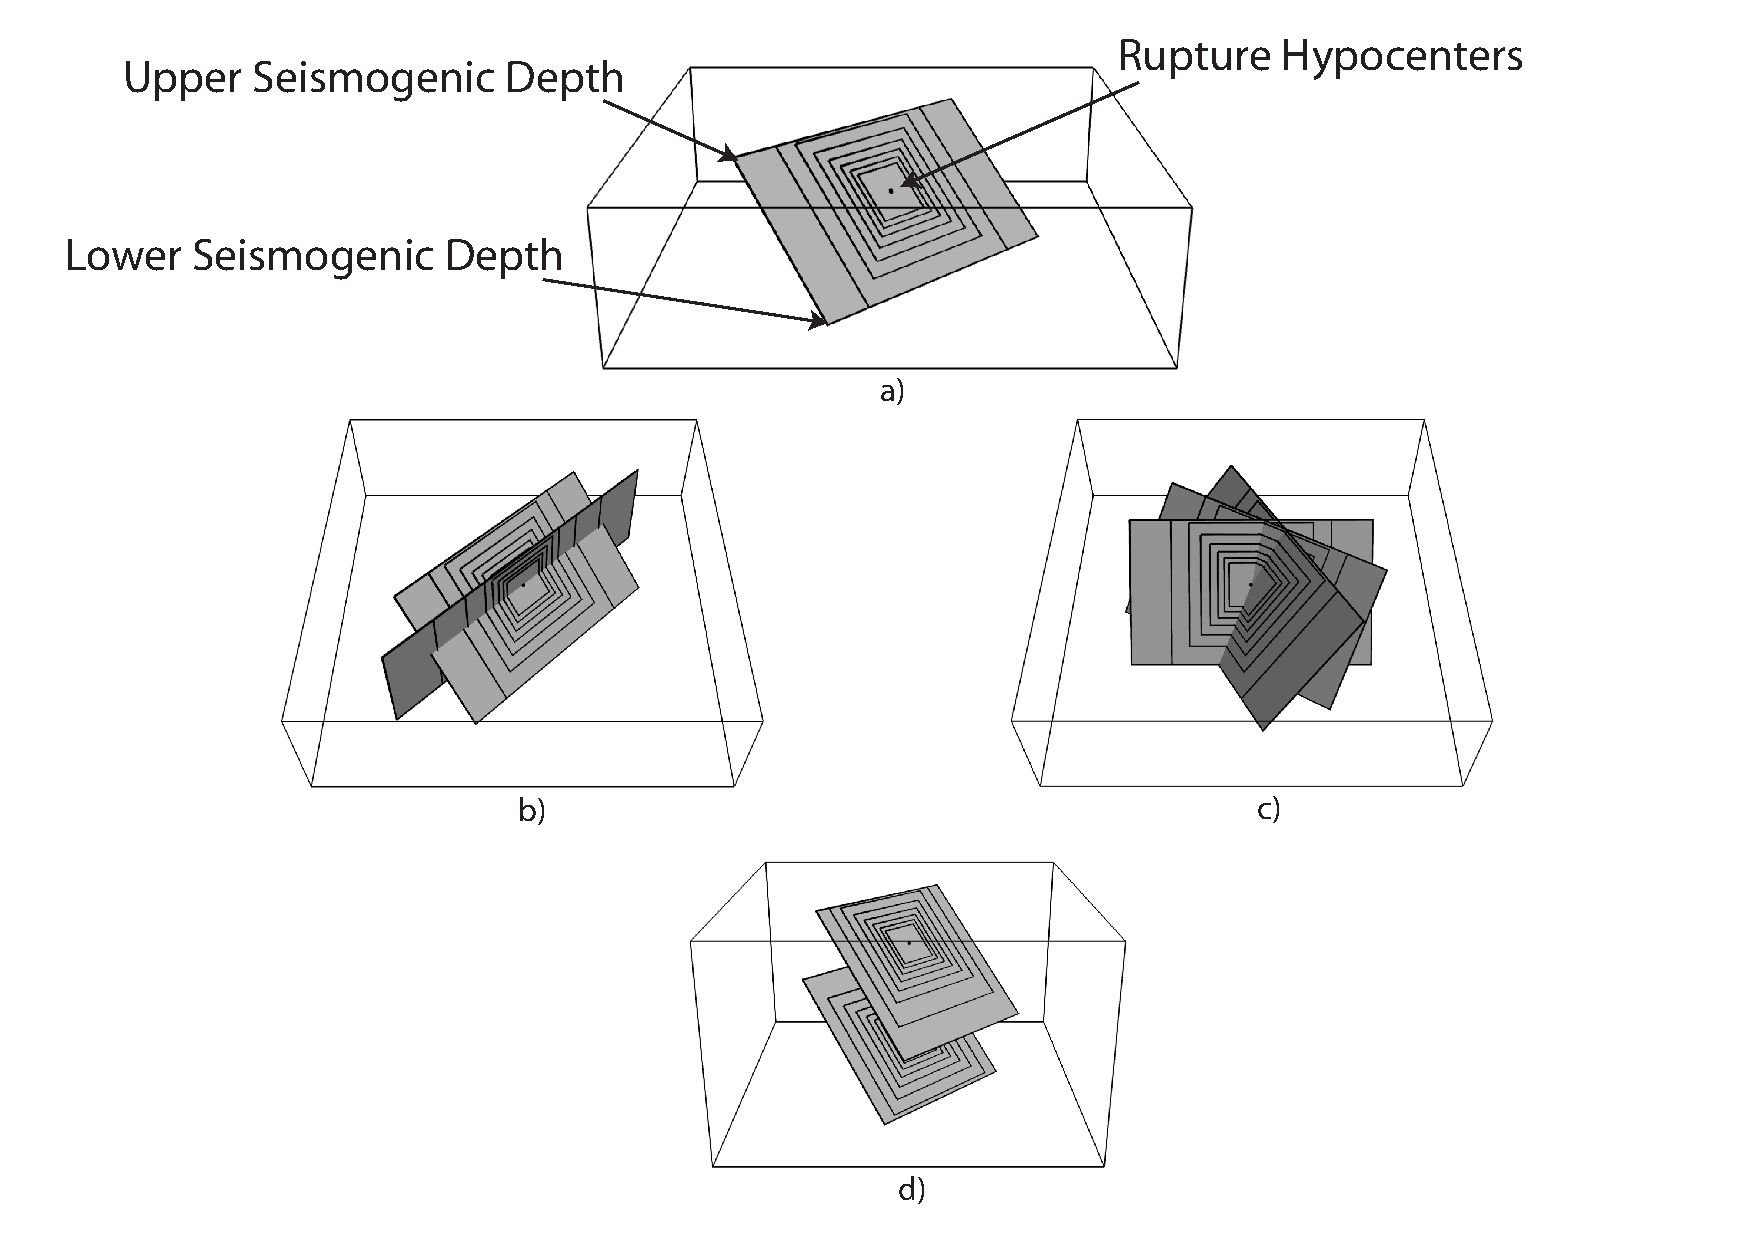
\includegraphics[width=14cm]{./Pictures/PointSource.pdf}
\caption{Graphical representation of the earthquake ruptures as generated by a
Point Source. a) Given a geographical location on the Earth surface, ruptures
are generated underneath according to a scaling relationship and aspect ratio
value and forced to not exceed the upper and lower seismogenic depths. Ruptures
can be distributed over multiple dips b), strikes c) and hypocentral depths
d).}
\label{fig:PointSource}
\end{figure}
Rupture centroids are co-located with the point-source location and are
positioned at depths specified by the hypocentral depth distribution. Rupture
shapes follow the given aspect ratio. However, if for a given aspect ratio and
hypocentral depth the rupture plane crosses either boundary (upper or lower) of
the seismogenic layer, the plane is shifted along the dip direction so as to fit
within the upper and lower seismogenic depths. As a consequence, the hypocentral
location no longer corresponds with the plane centroid. If this adjustment is
insufficient to avoid crossing either boundary of the seismogenic layer, the
plane is reshaped; the width becomes the maximum allowed by the seismogenic
layer thickness, and the length is increased so as to conserve rupture area (at
the expense of the aspect ratio).

In an area source (Figure \ref{fig:AreaSource}), earthquake ruptures are
distributed over a regular grid (equally-spaced in distance) covering a
geographical region as defined by a seismic zone. 
\begin{figure}
\centering
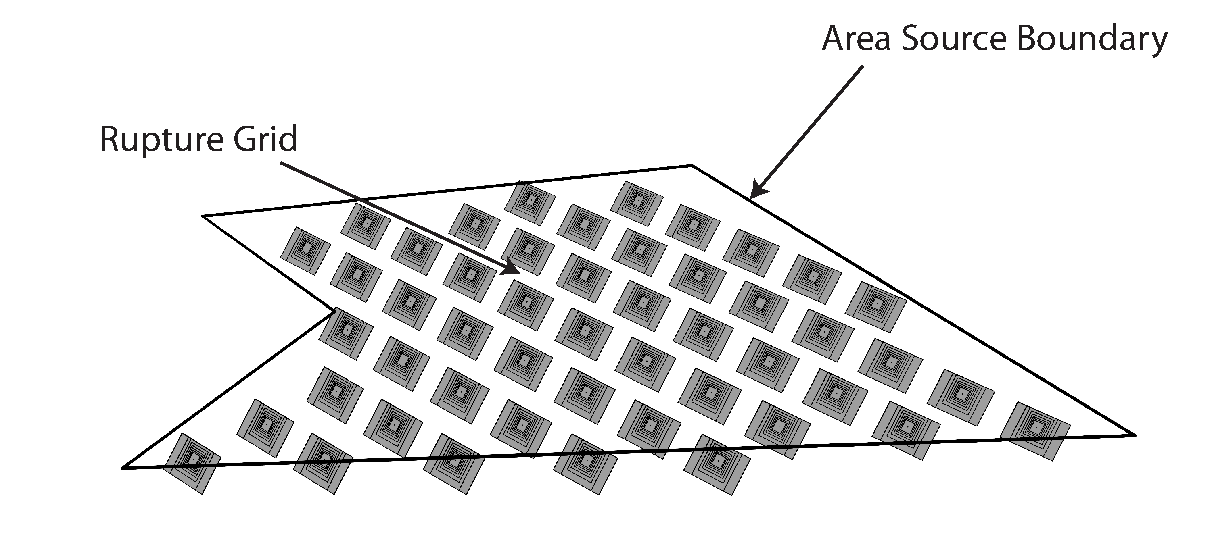
\includegraphics[width=14cm]{./Pictures/AreaSource.pdf}
\caption{Earthquake ruptures generated by an area source in the OQ-engine.
Ruptures are distributed uniformly over a regular grid within the area. In this
plot, for better visualization, ruptures are modeled only according to a single
nodal plane and hypocentral depth, but actual calculations may involve multiple
orientations and hypocentral depths. Ruptures originating from different grid
nodes may also overlap and cross each other.}
\label{fig:AreaSource}
\end{figure}
Generation of ruptures follows the same algorithm as for point sources.

For both sources, the rate associated to each rupture plane is the original rate
associated to the corresponding magnitude bin, scaled by the location weight (1
for a point source and 1/N for an area source, where N is the total number of
grid points in the area), the nodal plane (that is orientation and faulting
style) weight, and the hypocentral depth weight.

For an area source, the boundary is assumed ‘leaky’, that is earthquake ruptures
can extend out of it. Because of rupture area conservation, earthquake surfaces
associated to large magnitudes can extend well beyond the source boundaries. If
the rupture orientation is considered random then this behavior can potentially
lead to unrealistic scenarios, that is earthquake ruptures that are not
consistent with the area geometry and the tectonic feature it is meant to
represent. The design of an area source requires therefore a careful estimation
not only of the associated activity rates but also of the predominant faulting
orientations.

The OpenQuake-engine does not currently provide the possibility to define
non-leaky boundaries. The main difficulty in the implementation of such a
feature is the definition of a clear algorithm specifying how hard boundaries
would influence the generation of earthquake ruptures within the area source.
Several options are available. The easiest approach would be to remove, from the
set of generated ruptures, the ones that extend outside of the boundary. This
approach requires however a careful calculation of the occurrence rates to be
assigned to the earthquake ruptures. These cannot be calculated anymore
\textit{a priori} (that is from the number of grid points in the area source),
but only after all the ruptures have been generated and the ones crossing the
boundary excluded. Additionally, the removal of ruptures may also introduce a
non-uniform hazard pattern within the area source. An alternative approach would
be to truncate earthquake rupture surfaces that extend outside of the area
boundary. However, without a careful analysis of the consistency between the
main rupture orientations and source geometry, this approach may potentially
lead to large magnitude events developing over very small rupture surfaces. A
third approach would be to adjust the earthquake orientation/location so that
the rupture surface does not extend beyond the area boundary. Depending on the
source geometry, such an adjustment may not be always possible (that is, there
may no be an orientation/location which allows a rupture to fully lie within the
area source). This last strategy can be seen as a way to minimize the rupture
extension outside of the area source.

\section{The Simple Fault source}
\index{Seismic source!Simple fault}
Parameters required for the definition of a Simple Fault source are given in
Table \ref{table:simple_fault_tab}.
\begin{table}
\centering
\caption{Table summarizing parameters, and their functions, required for the
definition of a Simple Fault source in the OQ-engine}
\begin{tabular}{|p{60mm} p{60mm}|}
\hline
\rowcolor{anti-flashwhite}
\bf{Parameter} & \bf{Purpose} \\ \hline
Magnitude frequency distribution & Defines total moment rate and the relative
frequency of earthquakes of different magnitude\\
\hline
Temporal occurrence model & Defines functional form for the calculation of
the probability of the number of rupture occurrences in a given time span\\ 
\hline
Magnitude area scaling relationship & Define sizes and shapes of rupture planes \\
Rupture aspect ratio (length / width) & \\
\hline
Fault trace & Define fault surface \\
Upper seismogenic depth & \\
Lower seismogenic depth & \\
Dip angle & \\
\hline
Rake angle & Defines faulting style \\
\hline %inserts single line
\end{tabular}
\label{table:simple_fault_tab}
\end{table}
The fault surface is constructed by translating the fault trace (defined as the
intersection between the fault surface and the Earth s surface) from the upper
to the lower seismogenic depth along a direction perpendicular to the fault
trace strike (measured as the azimuth of the great circle line connection the first and last
coordinates of the trace) and with an inclination equal to the dip angle. The
surface so defined is effectively modeled as a regular (i.e. equally spaced in
distance) mesh (Figure \ref{fig:SimpleFaultSource}a).
\begin{figure}
\centering
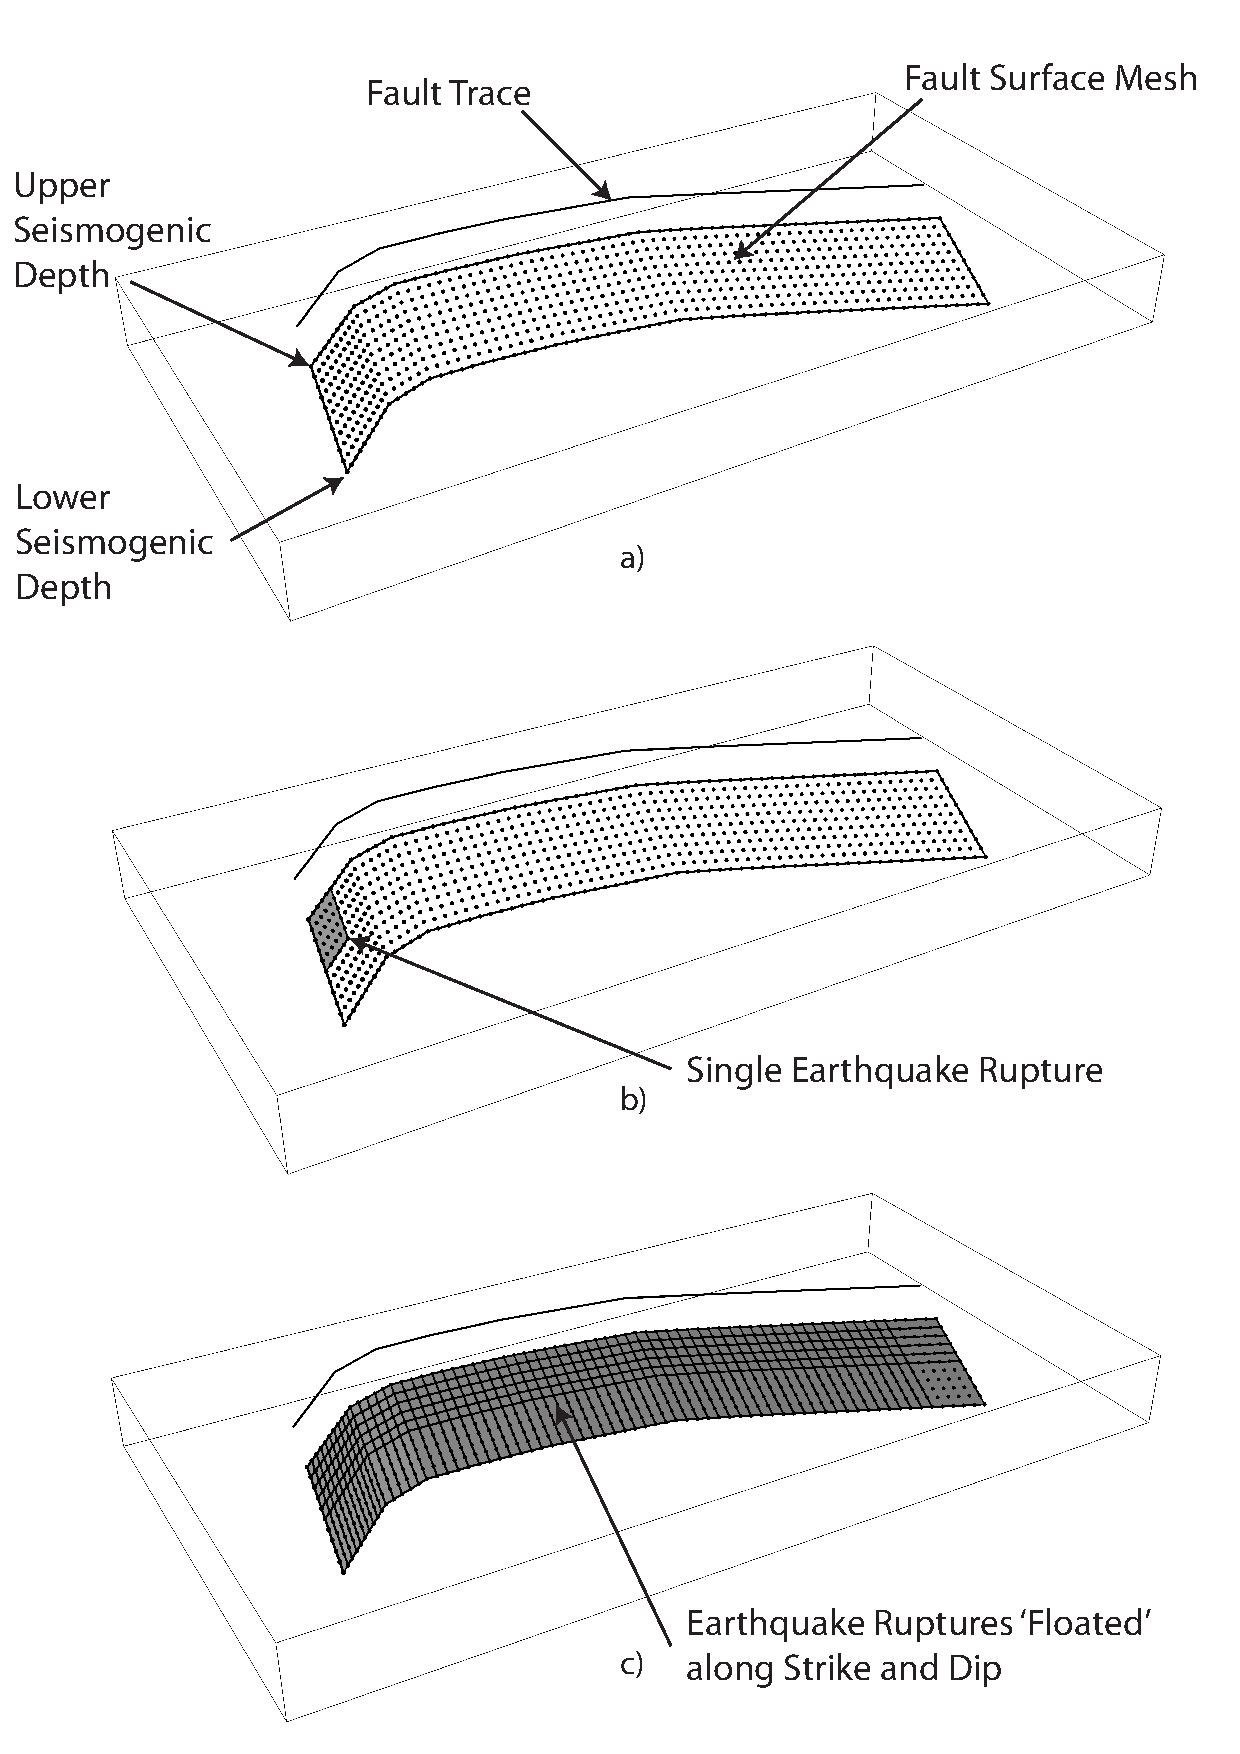
\includegraphics[width=14cm]{./Pictures/SimpleFaultSource.pdf}
\caption{Simple Fault source in the OQ-engine. The fault surface is obtained by
translating the fault trace from the Earth's surface to the lower seismogenic
depth with an inclination equal to the dip angle. The upper seismogenic depth
delimits the fault top edge. A mesh representation of the fault surface is then
constructed a). An earthquake rupture is defined as a portion of the fault
surface b), and all possible rupture locations are simulated by floating the
rupture surface both along strike and along dip c)}
\label{fig:SimpleFaultSource}
\end{figure}
For each magnitude bin defined in the magnitude-frequency distribution, an
earthquake rupture is modeled as a portion of the fault surface, accordingly
with the magnitude scaling relationship and the rupture aspect ratio (Figure
\ref{fig:SimpleFaultSource}b). To simulate all possible rupture locations, each
earthquake rupture is \textit{floated}, that is moved, along both the strike and
dip directions (Figure \ref{fig:SimpleFaultSource}c). 
%
The floating step is assumed equal to the mesh discretization step.  The
occurrence rate associated to a given magnitude bin is distributed uniformly
over all the ruptures associated with the same magnitude value.  \subsection{The
rupture floating algorithm for a Simple Fault source} We describe here in more
detail the algorithm adopted for modeling floating ruptures in a Simple Fault
source. We indicate with $\Delta$ the mesh spacing, and with
$n_{strike}^{fault}$ and $n_{dip}^{fault}$ the number of nodes along the strike
and dip directions in the mesh representing the entire fault surface. By
indicating with $L(M)$ and $W(M)$ the length and width of a rupture of magnitude
$M$ (obtained from equation \ref{eq:rup_l_w}), the equivalent number of nodes
(along strike and dip) representing a rupture on the mesh can be computed as:
\begin{equation} \label{eq:rup_nodes}
\begin{split}
& n_{strike}^{rup}(M) =  L(M) / \Delta + 1 \\
& n_{dip}^{rup}(M)     = W(M) / \Delta + 1 
\end{split}
\end{equation}
By further assuming that a rupture is floated along strike and dip with a step
equal to the mesh spacing ($\Delta$), we can compute the total number of
ruptures along strike and dip as:
\begin{equation}
\begin{split}
& N_{rup}^{strike}(M) = n_{strike}^{fault} - (n_{strike}^{rup}(M) - 1) \\
& N_{rup}^{dip}(M)     = n_{dip}^{fault} - (n_{dip}^{rup}(M) - 1)
\end{split}
\end{equation}
Since a rupture can propagate until its boundary reaches the fault boundary, but
not beyond, the total number of possible rupture locations along a certain
dimension is equal to the total number of nodes minus the number of nodes
required by the rupture reduced by 1, which represents the number of positions
that a rupture cannot occupy because it would otherwise extend, at least by one
mesh spacing, outside of the fault boundary.  Indicating with $\nu(M)$ the
annual occurrence rate as given by the magnitude-frequency distribution, the
annual occurrence rate associated to each rupture of magnitude $M$ is given by:
\begin{align}
\nu_{rup}(M) = \frac{\nu(M)}{N_{rup}^{strike}(M) * N_{rup}^{dip}(M)}
\end{align}
The occurrence rate scaling factor is therefore magnitude dependent (in contrast
with the Area Source where the scaling is constant for all magnitudes).
% ------------------------------------------------------------------------------
\section{The Complex Fault source}
\index{Seismic source!Complex fault}
Parameters required for the definition of a Complex Fault source are given in
Table \ref{table:complex_fault_tab}.
\begin{table}
\centering
\caption{Table summarizing parameters, and their functions, required for the
definition of a Complex Fault source in the OQ-engine}
\begin{tabular}{|p{60mm} p{60mm}|}
\hline
\rowcolor{anti-flashwhite}
\bf{Parameter} & \bf{Purpose} \\ \hline
Magnitude frequency distribution & Defines total moment rate and the relative
frequency of earthquakes of different magnitude\\
\hline
Temporal occurrence model & Defines functional form for the calculation of
the probability of the number of rupture occurrences in a given time span\\ 
\hline
Magnitude area scaling relationship & Define sizes and shapes of rupture planes
\\ 
Rupture aspect ratio (length / width) & \\
\hline
Top edge & Define fault surface \\
Intermediate edges (optional) & \\
Bottom edge & \\
\hline
Rake angle & Defines faulting style \\
\hline %inserts single line
\end{tabular}
\label{table:complex_fault_tab}
\end{table}
To accommodate the definition of irregular geometries, the Complex Fault source
requires the specification of the coordinates of, at least, the top and bottom
edges of the fault surface, and optionally, of one or more intermediate edges
(Figure \ref{fig:ComplexFaultSource}a). Edges can have different and variable
directions and a single edge can develop over different depth levels.  This
gives a very large flexibility in the definition of the fault surface, allowing
for changes in width and inclination both along strike and along dip.
\begin{figure}[!ht]
\centering
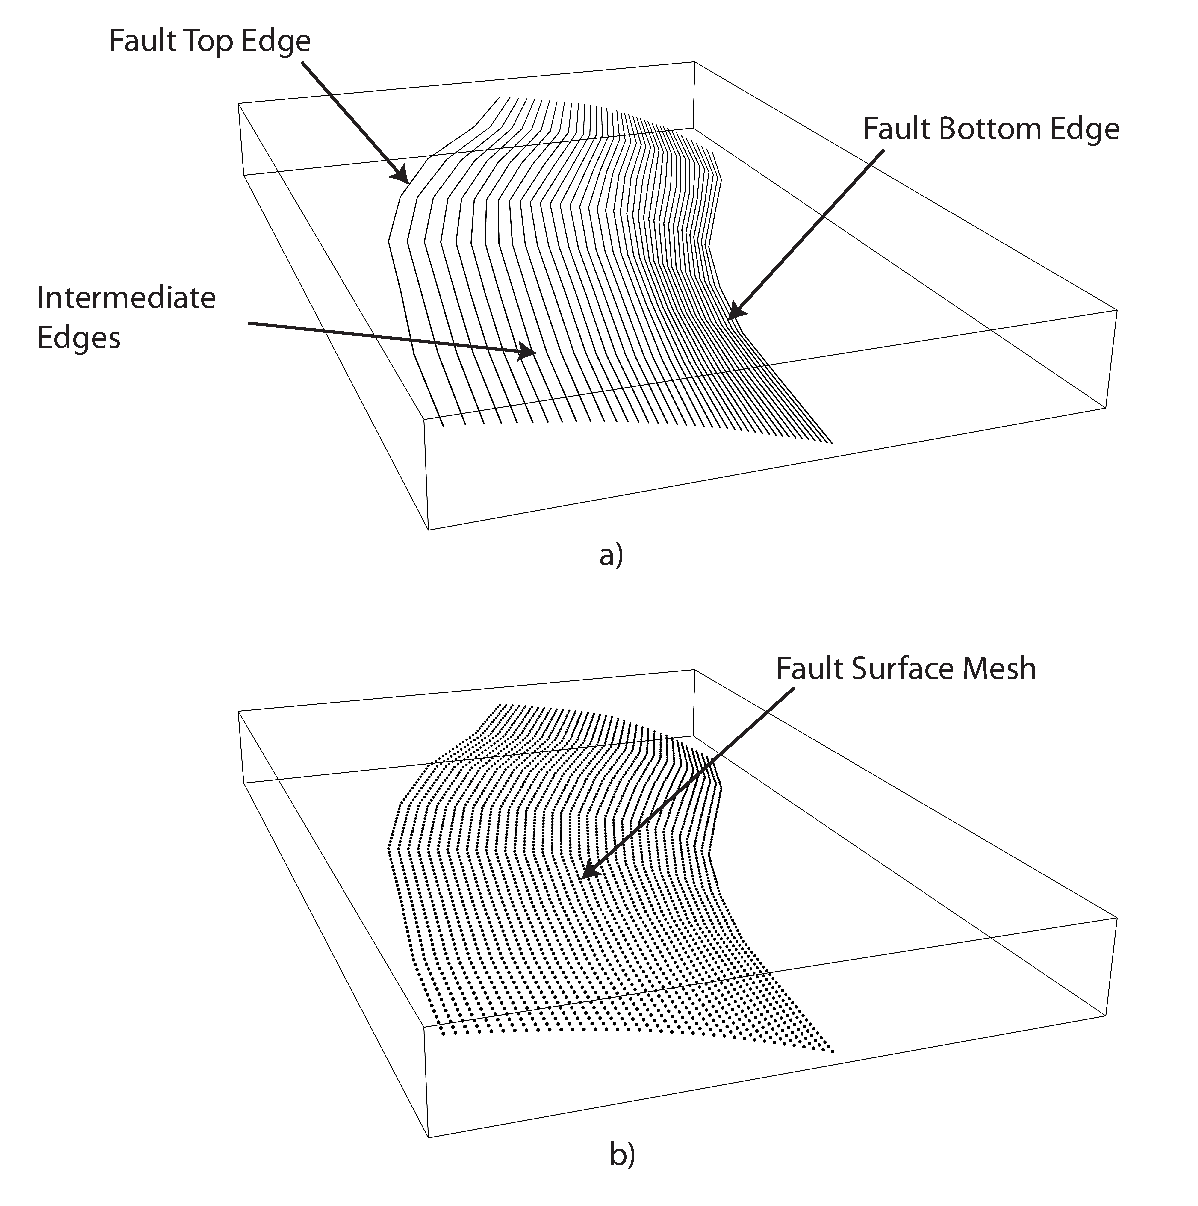
\includegraphics[width=14cm]{./Pictures/ComplexFault.pdf}
\caption{Complex Fault source}
\label{fig:ComplexFaultSource}
\end{figure}
%
% ------------------------------------------------------------------------------
\subsection{Mesh construction in a Complex Fault source}
The fault edges are used to construct a mesh representing the fault surface
(Figure \ref{fig:ComplexFaultSource}b). The mesh is, in general, not uniform;
that is, the mesh spacing may be spatially variable to accommodate the irregular
geometry of the surface.  The construction of the mesh relies on the following
algorithm. By indicating with $\overline{L}_{edge}$ the average edge length, and
with $\Delta$ the desired mesh spacing, the number of mesh points along the
strike direction is computed as:
\begin{align}
n_{strike} = \overline{L}_{edge} / \Delta + 1
\end{align}
Each edge is then resampled into $n_{strike}$ points. By connecting the
different edges along nodes that are on the same positions, dipping lines can be
constructed. By indicating with $\overline{W}_{fault}$ the average fault width
computed from the set of dipping lines, the number of mesh points along dip is
computed as: \begin{align}
n_{dip} = \overline{W}_{fault}/  \Delta + 1
\end{align}
Each dipping line is then resampled into $n_{dip}$ points. This completes the
construction of the mesh which is therefore represented by $n_{strike} \times
n_{dip}$ nodes. It is worth noticing how the resampling of the edges as well as
of the dipping lines allows the construction of a rectangular mesh which is
however non-uniform. The actual mesh spacing varies from values smaller than
$\Delta$, in regions where the fault length or width is smaller than the
corresponding average, to values larger than $\Delta$ where the opposite occurs.
$\Delta$, which is basically used to compute the number of nodes along strike
and dip, should therefore be considered as an \textit{average} mesh spacing.

\subsection{The rupture floating algorithm for a Complex Fault source}
The non-uniformity of the mesh representing the fault surface makes the rupture
floating algorithm for a Complex Fault source more problematic than for a Simple
Fault source. Indeed, because of the variation of the actual mesh spacing, it is
not possible to rely on the mesh spacing $\Delta$ to compute the number of nodes
required by a rupture of a given magnitude (that is equation
\ref{eq:rup_nodes}). For each possible rupture location, an optimization
procedure is used instead which identifies the number of nodes along strike and
dip which gives a mesh surface with an area that is the closest to the one
predicted by the magnitude area scaling relationship. In other words, the
rupture mesh is represented by a number of nodes which is not constant but that
may vary along the fault surface. In this context, the rupture aspect ratio is
used to define the length of the rupture top edge, while the rupture width
results from the optimization procedure. Such optimization procedure is well
exemplified in Figure \ref{fig:ComplexFaultSourcePanama}. The fault surface
represents a southward dipping subduction fault located north of Panama
defined in the model for South America developed by (\cite{petersen2010}). The
figures shows how a $M=7.7$ event is modeled in two different parts of the fault
surface. Where the fault is narrow (the western part) the rupture mesh contains
a large number of nodes, separated by a small distance. Where the fault is large
(the eastern part), the rupture mesh contains fewer nodes but separated by a
larger distance.
\begin{figure}
\centering
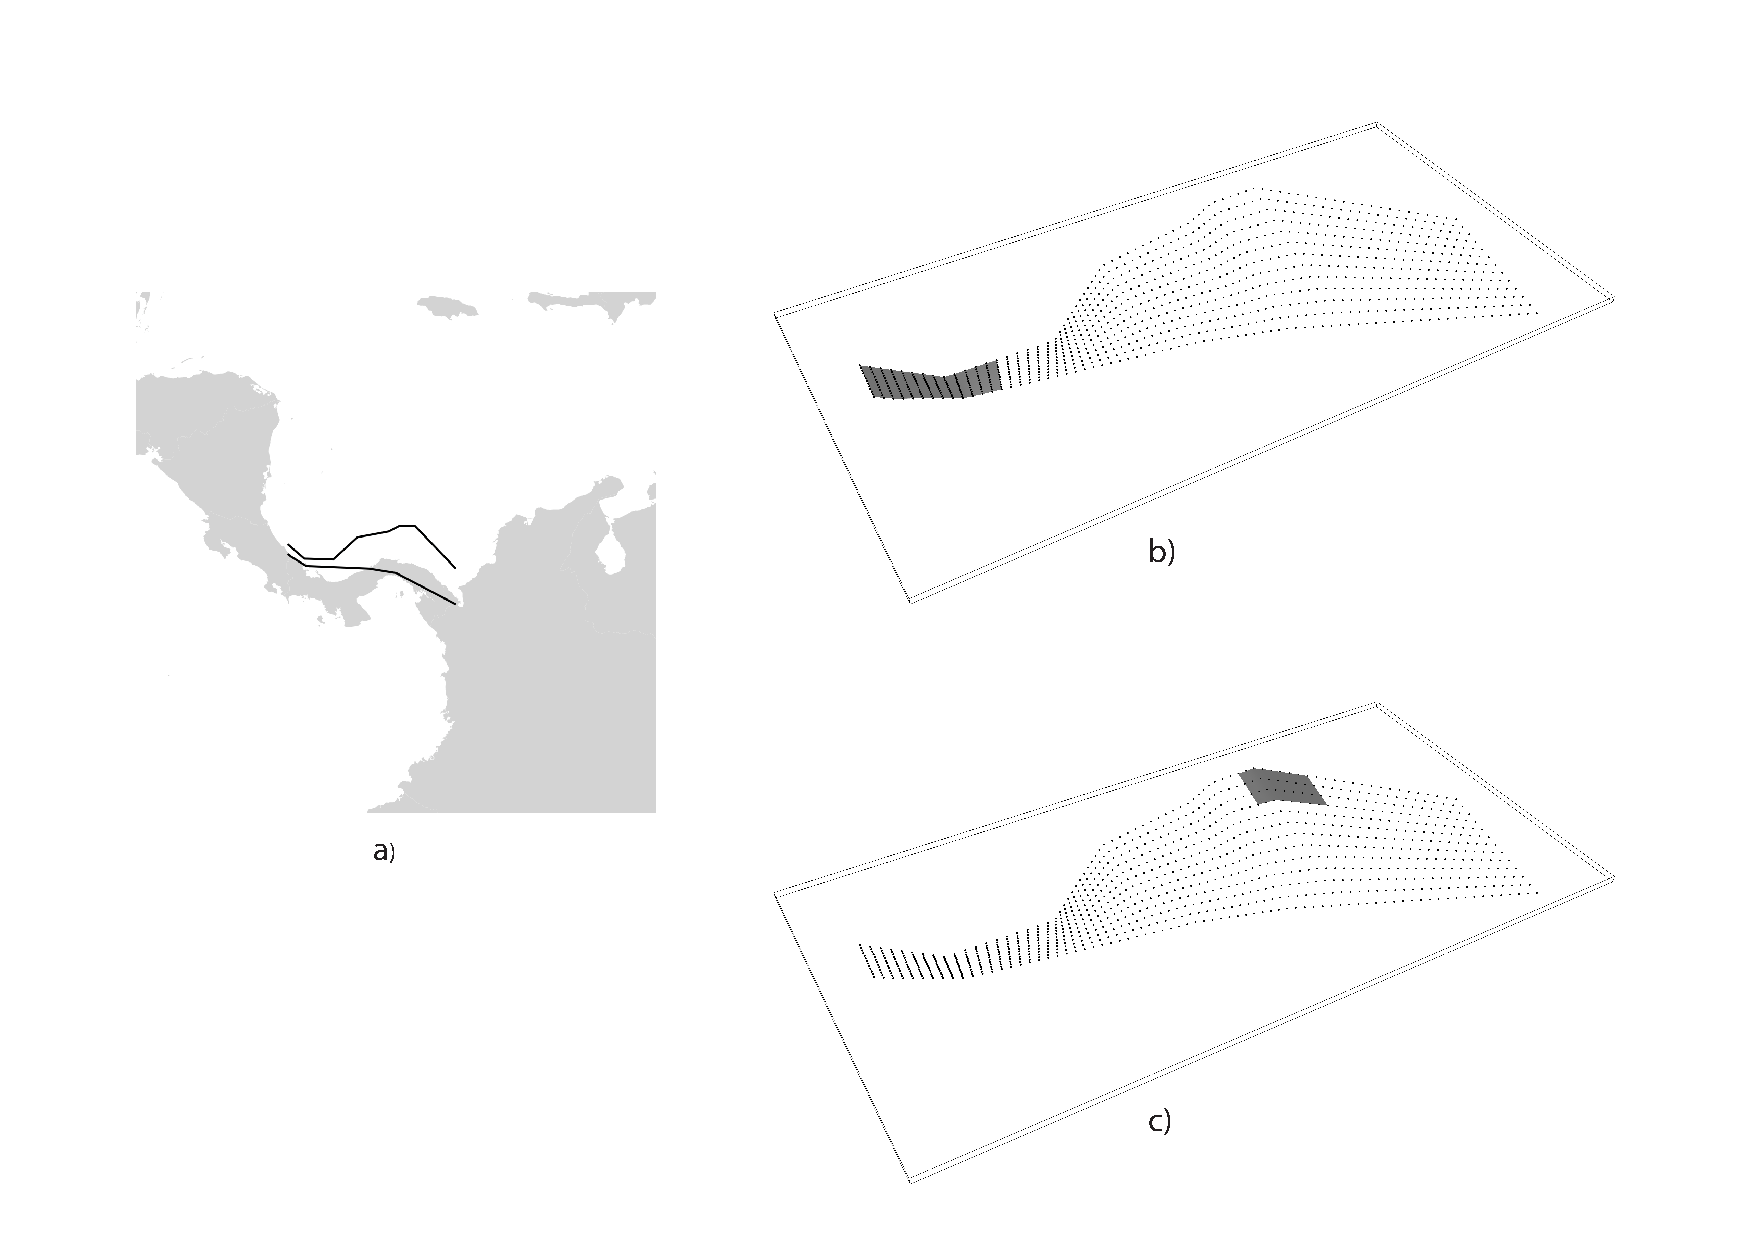
\includegraphics[width=14cm]{./Pictures/ComplexFaultPanama.pdf}
\caption{a) Example of Complex Fault source representing subduction interface
fault in North of Panama (\cite{petersen2010}). The mesh modeling a $M=7.7$
event is depicted in the eastern part b) and in the western part c)}
\label{fig:ComplexFaultSourcePanama}
\end{figure}
%
% ..............................................................................
\section{The Characteristic Fault source}
\index{Seismic source!Characteristic fault}
The \textit{Characteristic Fault} source is meant to represent individual faults
or fault segments that tend to produce earthquakes
\parencite{schwartscoppersmith1984} of essentially the same size. To offer the
greatest flexibility in the definition of the associated geometry, a
Characteristic Fault can be defined in terms of a simple fault geometry or as a
complex fault geometry. A third option is available, that is a collection of
planar ruptures, which can be used to model multi-segment ruptures for
instance (Figure \ref{fig:CharacteristicFaultSource}). In a Characteristic
fault, earthquake ruptures always break the entire fault surface, therefore the
rupture floating mechanism is not needed.  
\begin{figure}
\centering
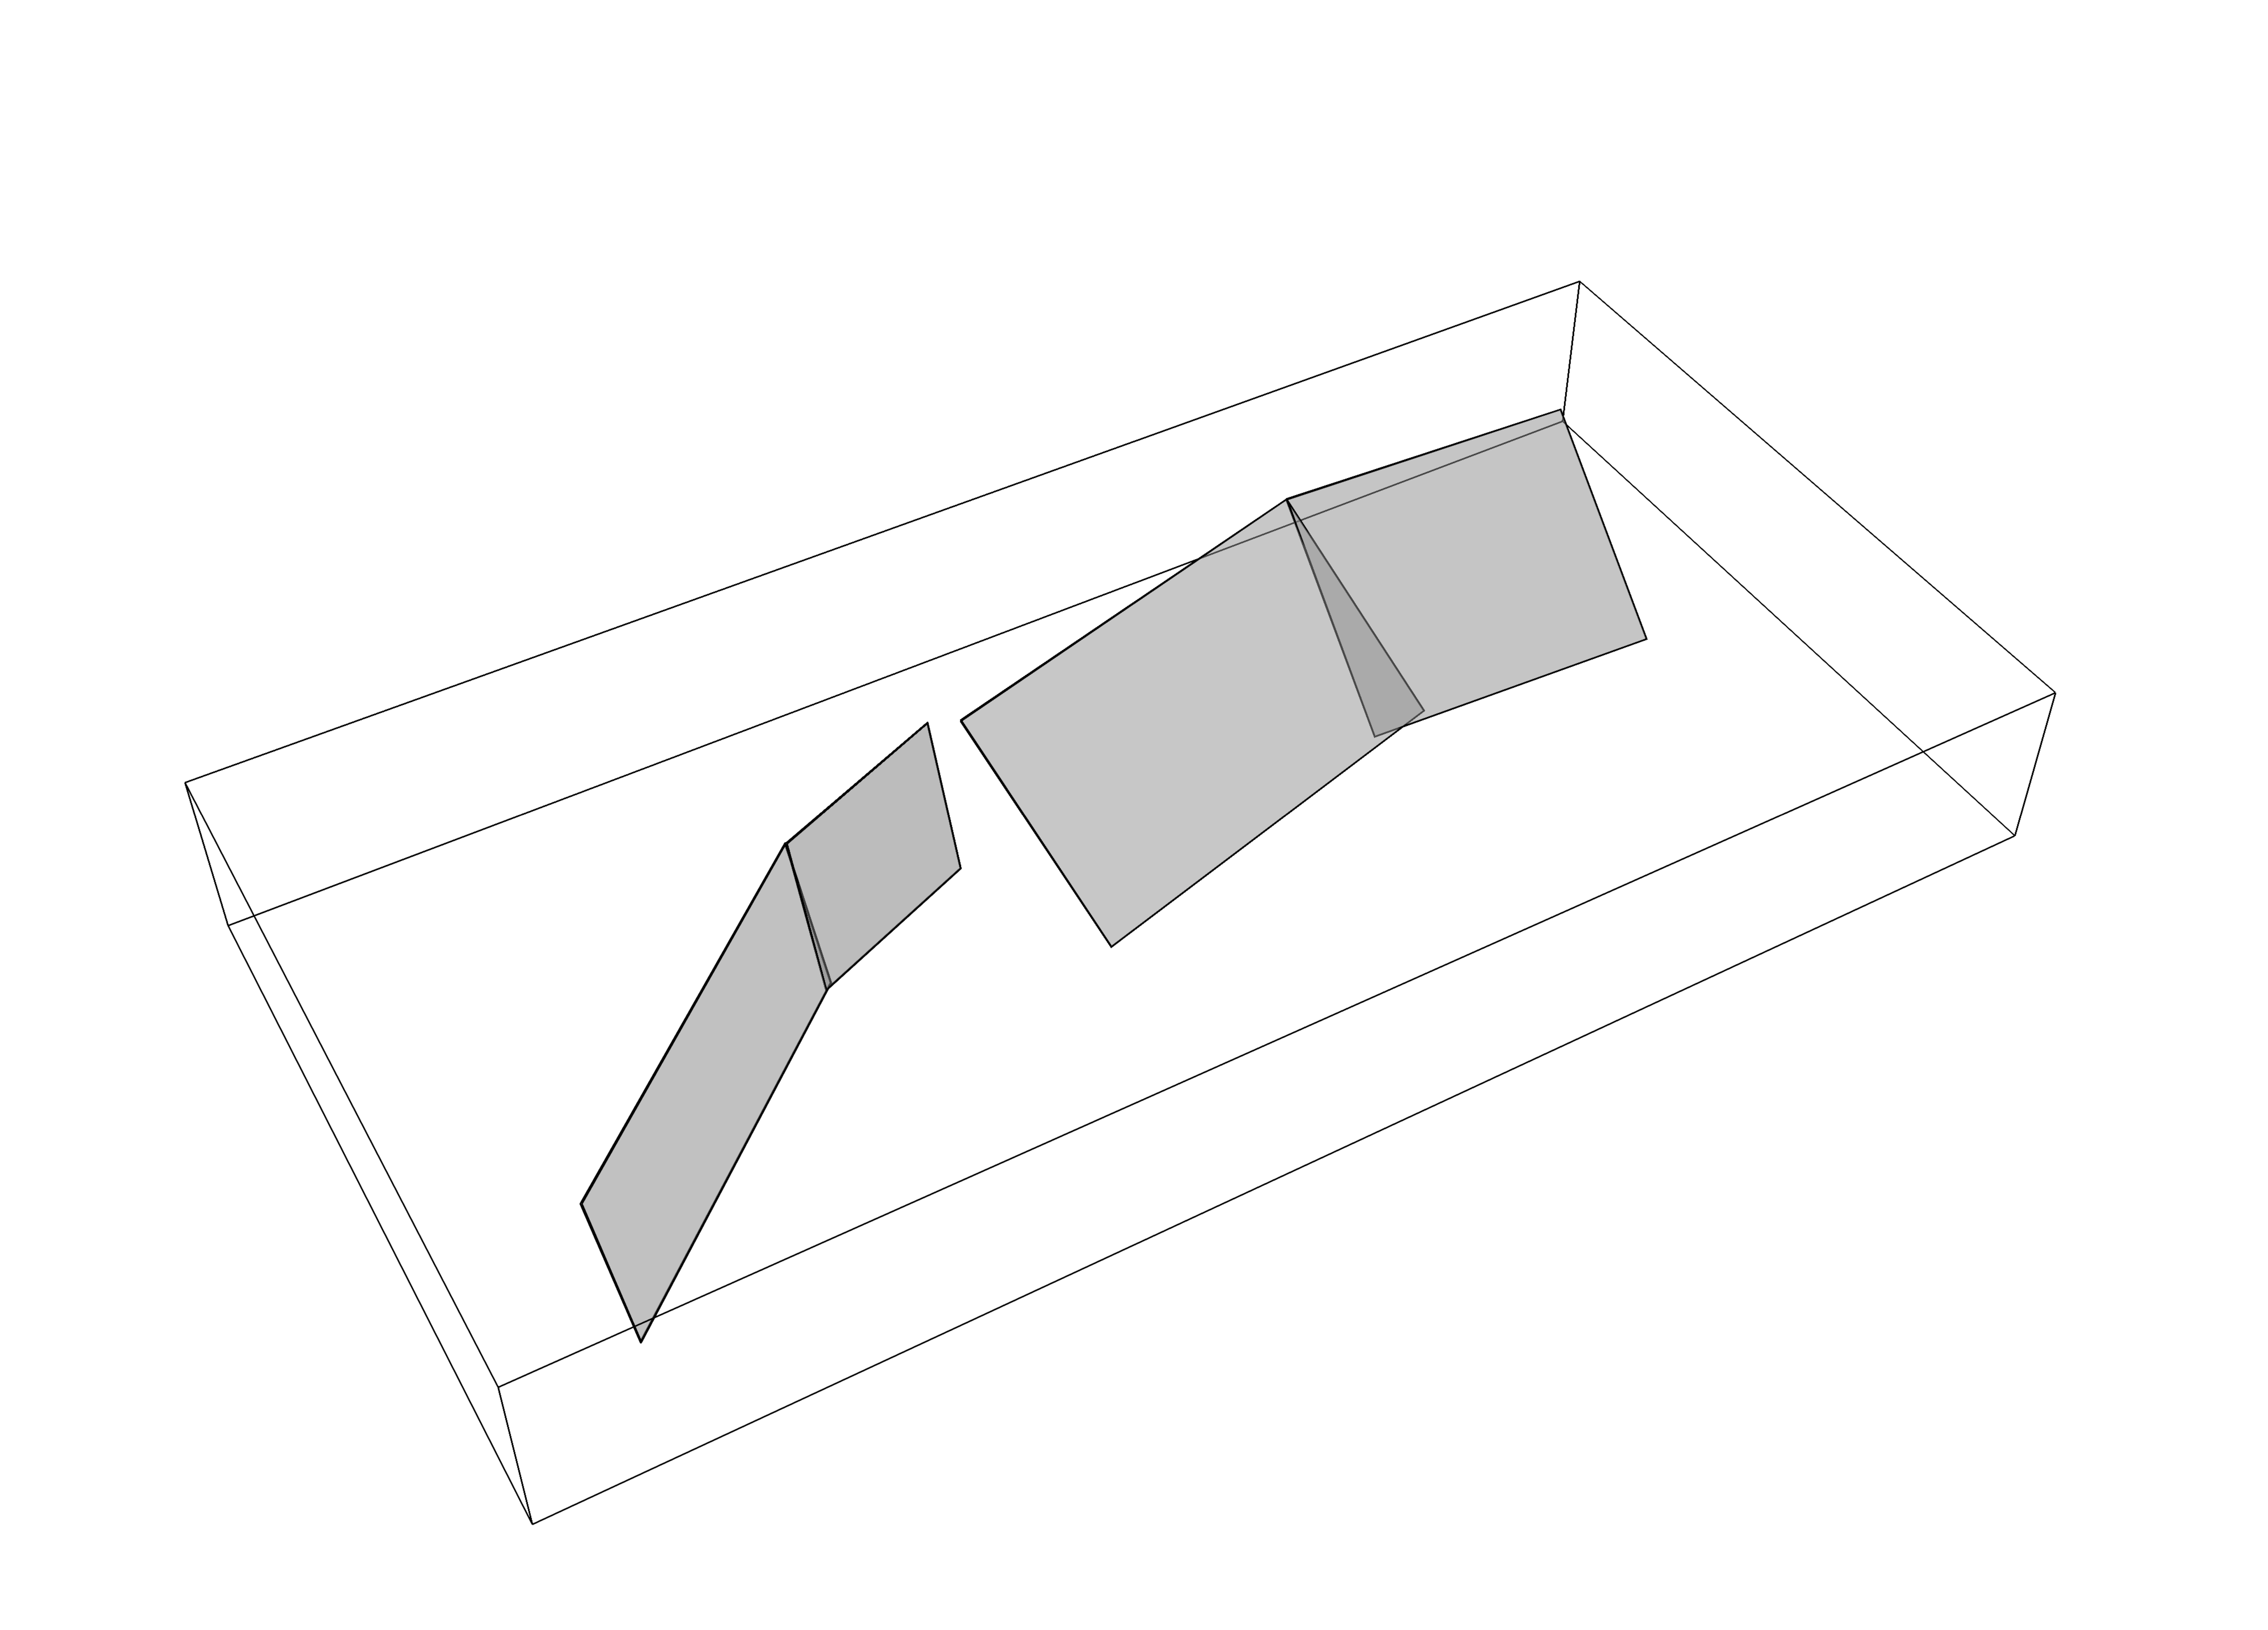
\includegraphics[width=14cm]{./Pictures/CharacteristicFaultSource.pdf}
\caption{Example of Characteristic Fault sources defined through a collection of
planar surfaces modeling a multi-segment rupture}
\label{fig:CharacteristicFaultSource}
\end{figure}


%----------------------------------------------------------------------------------------
%	CHAPTER 5
%----------------------------------------------------------------------------------------
\chapterimage{chapter_head_1.pdf} % Chapter heading image
\chapter{Ground Motion Prediction Equations}
\label{chap:gmpes}
This chapter provides an overview of ground shaking intensity modeling based 
on empirical equations and describes the way \glspl{acr:gsim} (more commonly 
known as ground motion models or \glspl{acr:gmpe}) are implemented in the 
\gls{acr:oqe}.
%
% ..............................................................................
\section{Introduction}
%
\Glspl{groundshakingintensitymodel} are empirical equations that - given a 
set of parameters - compute a value representative of the shaking 
intensity (or any other effect produced by an earthquake such as fault 
displacement) together with an associated uncertainty. 
%
\gls{acr:gsim} have a fundamental importance in the overall \gls{acr:psha} 
architecture.

A ground shaking intensity equation can be schematised as follows 
\parencite{alatik2010}: 
\begin{equation}
Y = f(X_{es},\theta)+\Delta
\end{equation}
where $Y$ is the natural logarithm of a ground shaking intensity measure, 
$X_{es}$ is the vector of explanatory (or independent) variables, $\theta$ 
is the vector of model coefficients and $\Delta$ is a random variable 
describing the overall variability of the ground shaking intensity at 
the site.

The selection of independent variables and the definition of the structure 
of the equation is usually done on the basis of physical principles and 
basic descriptions of the earthquake process, the latter
intended as the combination of a rupture occurrence, the synchronous 
radiation of seismic waves and their propagation to the site.
%
% . . . . . . . . . . . . . . . . . . . . . . . . . . . . . . . . . . . . . . .
\subsection{Main predictor variables}
\index{Ground-motion prediction equation!Predictor variables}
In the current section we give a brief overview of the most important predictor 
variables \cite[see][for a summary]{akkar2013r}supported by the \gls{acr:oqe}; 
currently they are organised into three main groups: variables describing the 
rupture properties, variables describing the rupture\--site path and variables 
used to characterise the site conditions. 
%
Table \ref{tab:parameters} contains a summary of the variables
assigned to the three groups.
% --------------------------------------------------------------------->>> Table
\begin{table}[!h]
\centering
\begin{tabular}{|p{5cm}p{8cm}|}
\hline
\rowcolor{anti-flashwhite}
\bf{Group} & \bf{Variables} \\
\hline 
Rupture parameters & - Magnitude\\
                   & - Dip \\ 
                   & - Z$_{tor}$ \\ 
                   & - Rake \\ \hline
Rupture-site distances & - See Table \ref{tab:distances} \\ \hline
Site parameters & - V$_{S,30}$ \\
                & - Depth to the 1 km/s interface interface \\
                & - Depth to the 2.5 km/s interface \\ 
\hline
\end{tabular}
\caption{Principal predictor variables supported by the \gls{acr:oqe} and 
    corresponding groups.}
\label{tab:parameters}
\end{table}
% ---------------------------------------------------------------------<<< Table
%
\subsubsection{Magnitude}
\index{Ground-motion prediction equation!predictor variables!Magnitude}
Moment magnitude \parencite{hanks1979} is the magnitude typology 
preponderantly used within the most recent \gls{acr:gsim} and as a 
consequence within seismic hazard analysis in general. 
%
However, in the \gls{acr:oqe} there is not a predefined magnitude typology.
It is up to the user to ensure that the magnitude used to define earthquake 
occurrence in the \gls{seismicsourcemodel} is consistent with the one used 
in the selected \glspl{groundshakingintensitymodel}.
%
\subsubsection{Distance}
\index{Ground-motion prediction equation!predictor variables!Source-site 
distance}
%
The OpenQuake-engine supports almost all the rupture-site 
distance metrics used by the most recent and complex 
\glspl{groundshakingintensitymodel} published in the scientific 
literature (see \ref{tab:distances} for a comprehensive list).
% --------------------------------------------------------------------->>> Table
\begin{table}[!b]
\centering
\begin{tabular}{p{5cm}cp{5cm}}
\hline
\rowcolor{anti-flashwhite}
\bf{Distance definition} & \bf{Symbol} & \bf{Description} \\
\hline 
Epicentral & R$_{epi}$ & \\
Hypocentral & R$_{hypo}$ & \\
Joyner and Boore distance & R$_{jb}$ & Closest distance from the surface 
    projection of the rupture \\
Rupture distance & R$_{rup}$ & Closest distance to the rupture surface \\
Horizontal top-edge distance & R$_{x}$ & Horizontal distance from the top 
    edge of the rupture \\
Top-of-Rupture depth & Z$_{tor}$ & Depth to the top edge of the rupture \\
\hline
\end{tabular}
\caption{Rupture-site distances supported by the \gls{acr:oqe}.}
\label{tab:distances}
\end{table}
% ---------------------------------------------------------------------<<< Table
The calculation of distances within the hazard component of the \gls{acr:oqe} 
is performed by assuming a spherical earth with a radius of 6371.0 km. 
%
\subsubsection{Rupture mechanism}
\index{Ground-motion prediction equation!Rupture mechanism}
Many \glspl{acr:gsim} compute ground-motion according to 
different categories identifying major rupturing mechanisms such as normal,
strike-slip or reverse.

In the \gls{acr:oqe} the rupture mechanism of a seismic source is specified 
in terms of the rake angle (defined according to \cite{aki2002}). 
%
Since the rake is not used directly as a predictor variable in 
\glspl{acr:gsim}, most of the \gls{acr:oqe} implementations contain a mapping
between the rake angle and the rupture mechanism classes supported by each
specific model.
%
\subsubsection{Time averaged shear-wave velocity in the uppermost 30m 
(V$_{S,30}$)}
\index{Ground-motion prediction equation!Rupture mechanism! Time averaged
shear-wave velocity in the uppermost 30m, V$_{S,30}$}
%
Local soil conditions and their effects on the ground-motion are routinely 
incorporated into \glspl{groundshakingintensitymodel} by means of a scalar
quantity corresponding to the time-averaged shear wave velocity measured 
in the uppermost 30m of the soil column (V$_{S,30}$).
%
Local soil conditions in the \gls{acr:oqe} are specified by means of this
parameter.

In case of \glspl{groundshakingintensitymodel} which support the definition 
of local soil conditions through soil classes (e.g. hard rock, soft soil) 
their implementation is done in a way that given a value of V$_{S,30}$ the
corresponding soil class is used to compute the value of ground motion 
(provided that a mapping between soil classes and V$_{S,30}$ is defined 
by the authors).

Additional parameters used to quantitatively describe local geology are 
the depths to the 1 km/s and 2.5 km/s shear-wave velocity interfaces. 
These are parameters used in some \glspl{acr:gsim} (e.g. \cite{chiou2008}) 
to quantify the overall thickness of the soil column. 
%
\subsubsection{Depth to the top-of-rupture (Z$_{tor}$)}
\index{Ground-motion prediction equation!Rupture mechanism!Depth to the top of
rupture}
The depth to the top of rupture is a parameter introduced in some of the NGA
West 1 \gls{acr:gsim} such as \textcite{chiou2008} and \textcite{abrahamson2008}
following a supposed dependence of ground-motion to the depth of the source,
as suggested by \textcite{somerville2006a}.
%
% ..............................................................................
\section{Use of GMPEs in seismic hazard analysis}
% 
The standard process adopted for the implementation into the \gls{acr:oqe} 
of a \gls{groundshakingintensitymodel} requires a 
set of verification tables which contain values of ground-motion (or standard 
deviation) computed using a large number of the possible predictor 
variables combination. 

Through these tables and an automated verification procedure, it is 
possible to achieve with a high confidence level the consistency between 
the original results and the corresponding values computed with the 
version of the \gls{acr:gsim} implemented.
%
% . . . . . . . . . . . . . . . . . . . . . . . . . . . . . . . . . . . . . . .
\subsection{Testing}
%
The progressively increasing complexity of \glspl{groundshakingintensitymodel}
is giving more and more emphasis and relevance to the validation between 
between the results provided by the \gls{acr:gsim} implemented in
\gls{acr:psha} codes and the results of original implementations 
described in the scientific literature or directly provided by the authors.

The \gls{acr:oqe} provides an automated procedure for the testing of 
the implemented \glspl{groundshakingintensitymodel}. 
%
% . . . . . . . . . . . . . . . . . . . . . . . . . . . . . . . . . . . . . . .
\subsection{Selection criteria}
The number of published \gls{acr:gsim} increased exponentially over the last
few years.  
%
\subsubsection{Pre-selection criteria}
\cite{cotton2006} 

%
\subsubsection{Selection criteria}
%
%
% ..............................................................................
\section{Calculation of ground motion fields}
%
The calculation of \glspl{groundmotionfield} is an essential step in the
calculation of hazard via an \gls{epsha} and for the calculation of losses 
in case of spatially distributed assets.
% . . . . . . . . . . . . . . . . . . . . . . . . . . . . . . . . . . . . . . .
\subsection{Spatial correlation of ground motion}
%
% ..............................................................................
\section{Modified GMPEs}
%
% . . . . . . . . . . . . . . . . . . . . . . . . . . . . . . . . . . . . . . .
\subsection{Adjusted equations}
%
% . . . . . . . . . . . . . . . . . . . . . . . . . . . . . . . . . . . . . . .
\subsection{Non-ergodic sigma}
%
% ..............................................................................
\section{Future developments}
%
% . . . . . . . . . . . . . . . . . . . . . . . . . . . . . . . . . . . . . . .
\subsection{Sigma adjustment}
%
% . . . . . . . . . . . . . . . . . . . . . . . . . . . . . . . . . . . . . . .
\subsection{Vs-Kappa correction}
%
% . . . . . . . . . . . . . . . . . . . . . . . . . . . . . . . . . . . . . . .
\subsection{Host-to-target adjustment}
%
% . . . . . . . . . . . . . . . . . . . . . . . . . . . . . . . . . . . . . . .
\subsection{Spatial cross correlation}
%
% . . . . . . . . . . . . . . . . . . . . . . . . . . . . . . . . . . . . . . .
\subsection{Near source directivity effects}



%----------------------------------------------------------------------------------------
%	CHAPTER 6
%----------------------------------------------------------------------------------------
\chapterimage{chapter_head_1.pdf} % Chapter heading image
\chapter{Logic-trees}
%
\index{Logic-tree}
The logic-tree is an integral component of a PSHA input model for the 
OpenQuake-engine.  

An Openuake-engine hazard input model always contains a logic tree structure 
which describes the epistemic uncertainties associated with the construction 
of the seismic source model and a logic-tree used to formally specify 
epistemic uncertainties related to \gls{acr:gsim} models to be used in 
different tectonic regions.

The definition of logic trees in the OpenQuake-engine is based on
the combination of a number of predefined modules each one modelling a specific
epistemic uncertainty. Two are the main advantages of this approach. The first
and most evident is that the user is not forced to use a predefined logic tree
structure and - instead - can create a specific logic tree which reflects the 
uncertainties they defined. The logic tree structure become an integral part of
the definition of a PSHA input model. The hazard calculations with this approach
become fully reproducible and do not require pre- or post-processing steps.

This Chapter is dedicated to the description of the basic theory behind 
logic-trees and to the delineation of how logic-trees are implemented 
into the OpenQuake-engine.
%
% ..............................................................................
\section{Introduction (meaning and interpretation)}
The use of logic-trees to account for epistemic uncertainties in a 
probabilistic seismic hazard analysis was originally proposed by 
\textcite{kulkarni84}.
%
Nowadays they are an essential component of a \gls{acr:psha} input
model and represent the formal methodology though which is possible to 
synthesize the results of the epistemic uncertainties elicitation process
requested in site-specific seismic hazard analyses \parencite{budnitz1997}
as well as state\--of\--the\--art national and regional \gls{acr:psha} 
input models. 
%
% ..............................................................................
\section{The OpenQuake-engine logic-tree structure}
%
The \gls{acr:oqe} provides with the user a flexible and modular methodology 
to create model specific logic-tree structures. Logic-trees are defined as a
set of linked modules which starting from the roots get to the uppermost 
branches.
%
% . . . . . . . . . . . . . . . . . . . . . . . . . . . . . . . . . . . . . . .
\subsection{The seismic source model logic tree}
The seismic source model logic tree handles the epistemic uncertainties
related to the definition of geometry, position and seismicity occurrence 
properties of seismic sources. 

Logic-trees are a tool designed to consider in a systematic manner the 
epistemic uncertainties of models and parameters included in a hazard 
analysis.
% ..............................................................................
% . . . . . . . . . . . . . . . . . . . . . . . . . . . . . . . . . . . > Figure
%\renewcommand{\psedge}{\ncdiag[armA=0,angleB=180,armB=1cm]}
\begin{figure}[!hb]
%\hfill \\
\textcolor{airforceblue}{\emph{Branch set definition}}: \dotfill Simple Fault 
	Dip Angle \\
\textcolor{airforceblue}{\emph{Branch set uncertainty type}}: \dotfill 
	Absolute values \\
\textcolor{airforceblue}{\emph{Applies to}}: \dotfill Simple faults \\
\textcolor{airforceblue}{\emph{Correlated branches}}: \dotfill Yes \\
\hfill \\
% Tree
\centering
\begin{pdfpic}
\begin{psTree}[treemode=R,levelsep=*2cm]
\end{psTree}%
\end{pdfpic}
\\ \hfill \\


\caption{An example of branch set used to account for the epistemic 
uncertainties on faults dip angle; in this case each branch contains a value 
of the dip.}
\label{fig:logic_tree_branching_levels}
\end{figure}

%
\subsubsection{Supported epistemic uncertainties}

\begin{description}
\item [Source model] models the uncertainty on seismic source model e.g. models
with different geometries of sources covering the same region.
\item [maxMagGRRelative]
\item [bGRRelative] models relative uncertainty on the b-value of a
double-truncated Gutenberg-Richter relationship.
\item [abGRAbsolute]
\item [maxMagGRAbsolute]
\end{description}
%
% . . . . . . . . . . . . . . . . . . . . . . . . . . . . . . . . . . . . . . .
\subsection{The ground-motion model logic tree}
%
\subsubsection{Supported epistemic uncertainties}
Currently the only epistemic uncertainty allowed for the \gls{acr:gsim}
logic-tree.
%
% ..............................................................................
\section{Logic tree processing}
The \gls{acr:oqe} currently provides two distinct ways to process logic-trees
%
\subsection{Full-path enumeration}
Full-path enumeration is the simplest logic-tree processing methodology
implemented. The use of this methodology is possible only when the logic tree
structure is relatively simple i.e. the number of end branches is small. 
%
\subsection{Monte Carlo sampling}
Monte Carlo sampling is the processing methodology 
%
\subsection{Logic tree pruning/collapsing}
\subsection{Calculation of mean and percentiles/quantiles}


%----------------------------------------------------------------------------------------
%	CHAPTER 6
%----------------------------------------------------------------------------------------
%\chapterimage{chapter_head_1.pdf} % Chapter heading image
%\chapter{Calculators and outputs description}
%This chapter presents practical examples of PSHA done with the OQ-engine. By considering simple synthetic test cases, we illustrate the behaviour of a number of algorithms underlying the seismic source modelling
and the logic tree processing. We also present examples of PSHA performed using the national seismic hazard model for U.S. (\cite{petersen2008}) to illustrate the capabilities of the OQ-engine when dealing with complex
models.

\section{Classical PSHA with an Area Source}
We consider here the case of a single area source. The source has a circular shape of 200 km radius. The activity
is described by a truncated Gutenberg-Richter magnitude frequency distribution, with minimum magnitude
equal to 5 and maximum magnitude equal to 6.5. The \textit{a-value} is 5 (i.e. the source generates one
event per year with $M \ge 5$) and \textit{b-value} is 1. The seismogenic layer extends from 0 to 20 km.
Ruptures are associated to a single hypocentral depth (10 km) and nodal plane (strike 0, dip 90, rake 0).

\subsection{The area source discretization step}
We study here the effect of the area source discretization step ($\Delta$) in the calculation of hazard map values. That is, we investigate the effect that the spacing used to discretize the region delimited by the area
source boundary has on hazard levels corresponding to a given probability of exceedance. We thus compute
hazard curves (for PGA) on a set of locations equally spaced by 10 km defing a profile crossing the centre of the area source, from east to west.

We compute hazard curves using different GMPEs (\cite{boore2008}, \cite{chiou2008}, \cite{campbell2008} and \cite{abrahamson2008}) to investigate the potential dependence of the results accuracy on the ground motion model. From the hazard curves we extract PGA values corresponding to 10 \% in 50 years. Results for four discretization levels (20, 10, 5, and 2.5 km) are show in
Figure \ref{fig:delta_area}. When using $\Delta=20$ km, the hazard map values show strong fluctuations
 (where the highest are for the \cite{boore2008} model) within the area region (that is in the distance
range [-200, 200] km). For discretization steps equal to or smaller than 10 km, the different solutions converge instead to the same values.
\begin{figure}
\centering
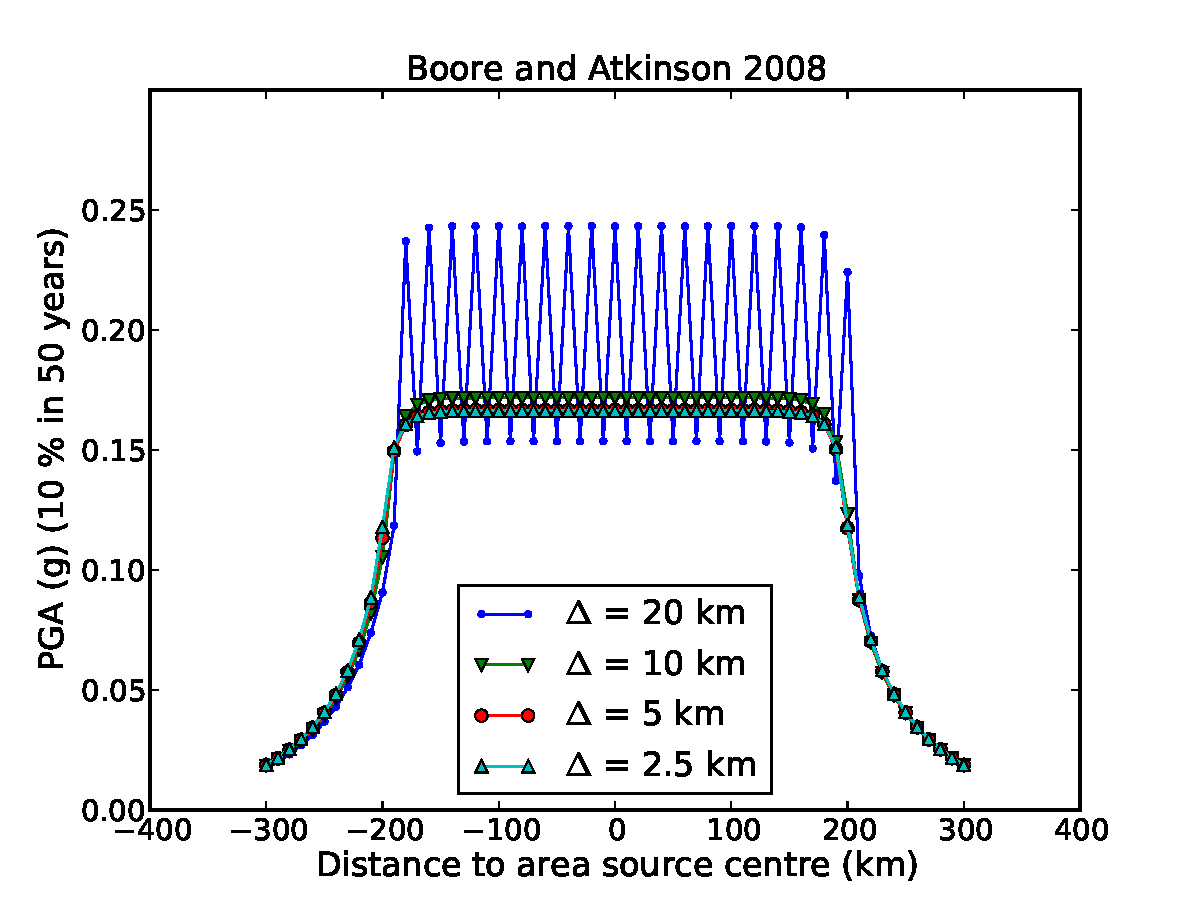
\includegraphics[width=7cm]{./Pictures/PGA_0pt1_source_model_a5_BA2008.pdf}
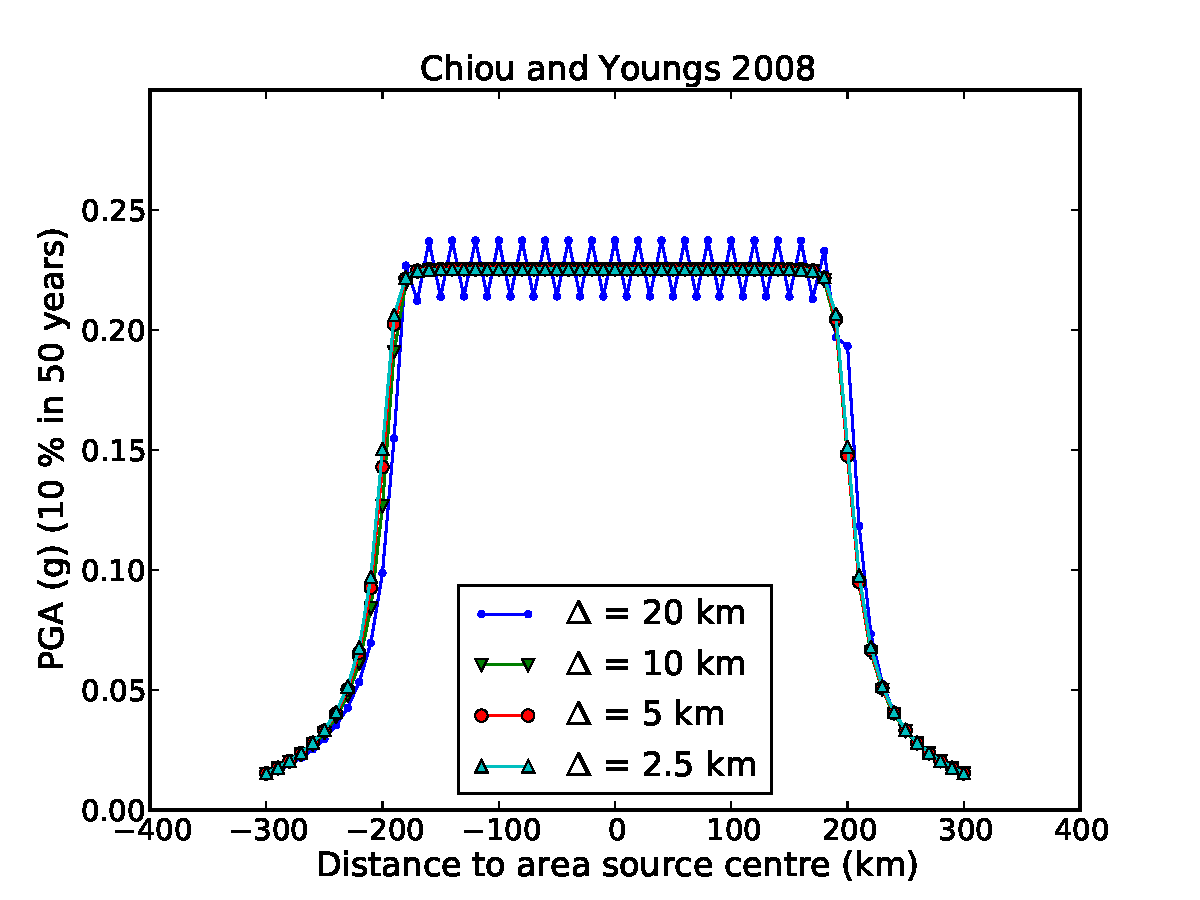
\includegraphics[width=7cm]{./Pictures/PGA_0pt1_source_model_a5_CY2008.pdf}
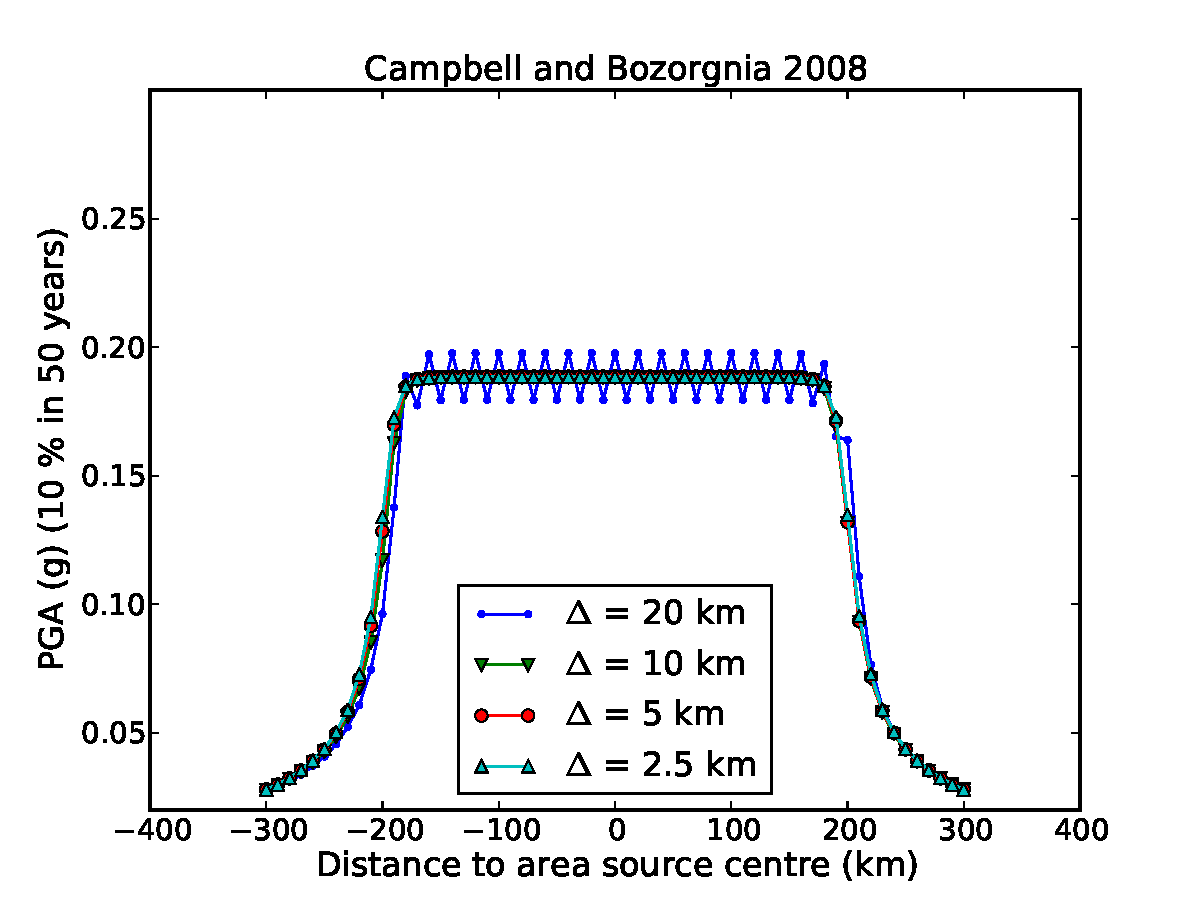
\includegraphics[width=7cm]{./Pictures/PGA_0pt1_source_model_a5_CB2008.pdf}
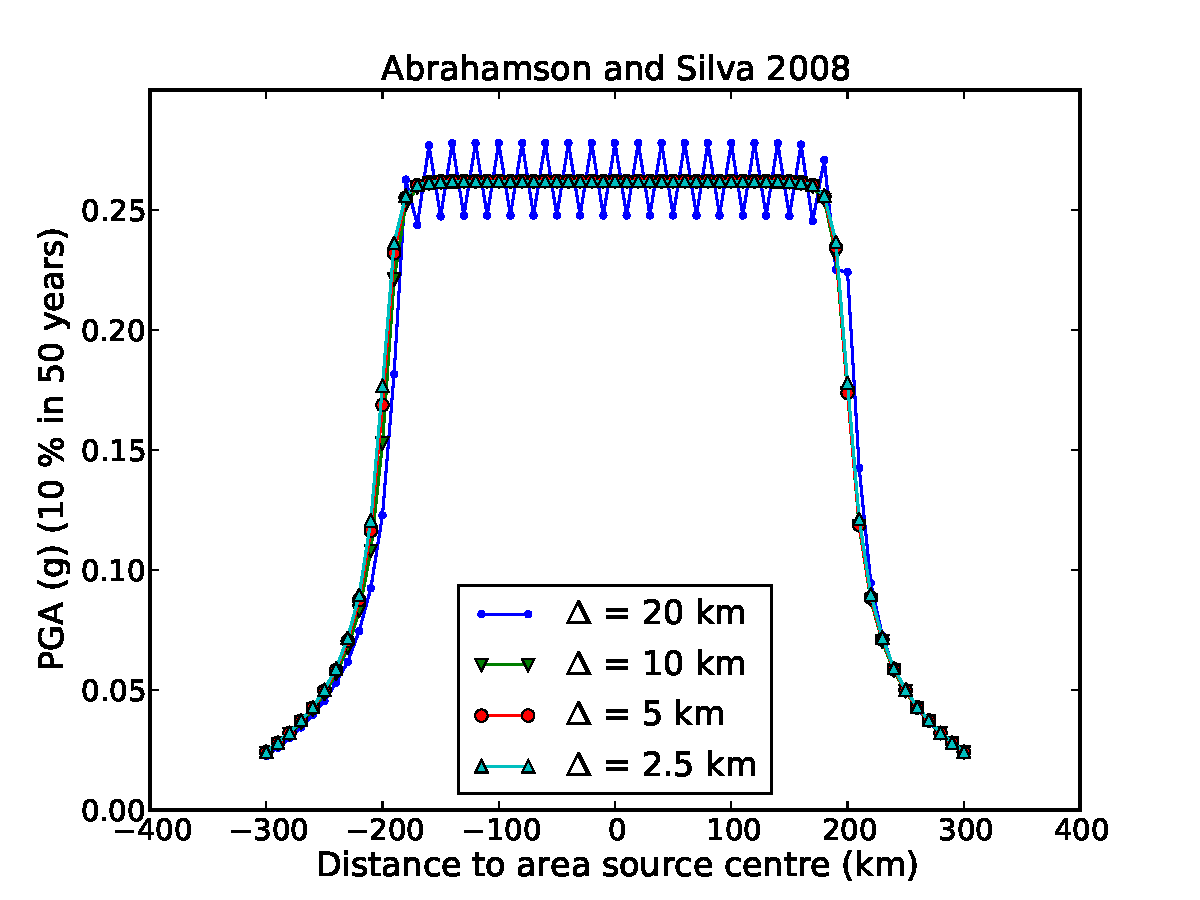
\includegraphics[width=7cm]{./Pictures/PGA_0pt1_source_model_a5_AS2008.pdf}
\caption{The effect of the area source discretization step ($\Delta$) on hazard map calculation}
\label{fig:delta_area}
\end{figure}

\subsection{The effect of dip and rake angles}
To investigate the effect of modelling earthquake ruptures with different inclination (that is dip angle) and
faulting style (rake angle), we compare here hazard map values for an area source generating only vertical,
strike-slip ruptures and an area source generating dipping (dip=$50^{\circ}$), reverse (rake=$90^{\circ}$) ruptures.

To investigate the potential dependence on the source seismic activity level, we compute hazard maps for
area sources having different Gutenberg-Richter a values ($a_{GR}$) equal to 3, 4 and 5, corresponding to
annual occurrence rates above $M=5$ of 0.01, 0.1 and 1, respectively. Results are shown in Figure \ref{fig:dip_rake_area}. Sensitivity of rupture dip and faulting style clearly depends on the source activity level and on the GMPE model. Independently of the GMPE, the highest absolute difference in PGA is for the highest $a_{GR}$. Among the different GMPE models, \citet{campbell2008} shows the highest sensitivity (about 20 %
increase in PGA at $a_{GR}=5$), while \citet{boore2008} shows the lowest sensitivity.
\begin{figure}
\centering
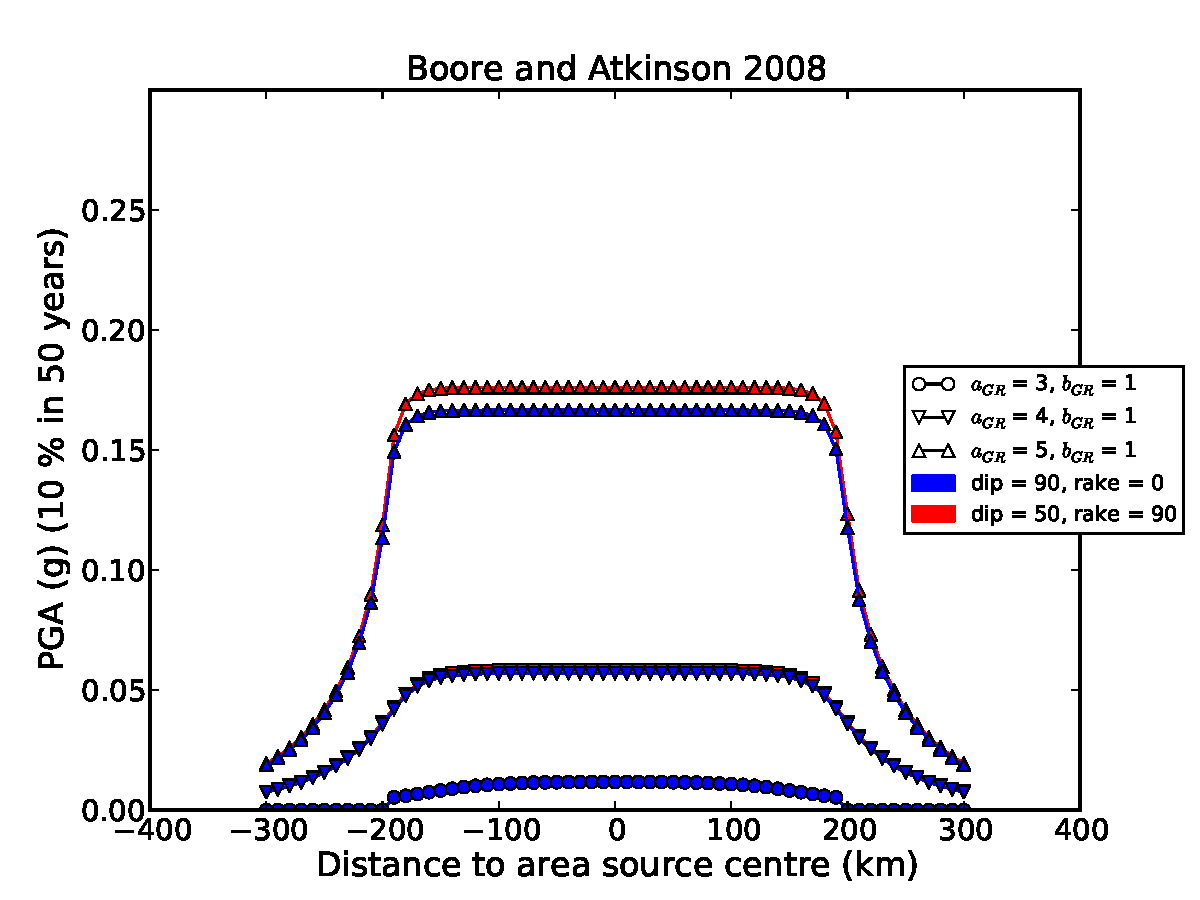
\includegraphics[width=7cm]{./Pictures/PGA_0pt1_BA2008_dip_rake.pdf}
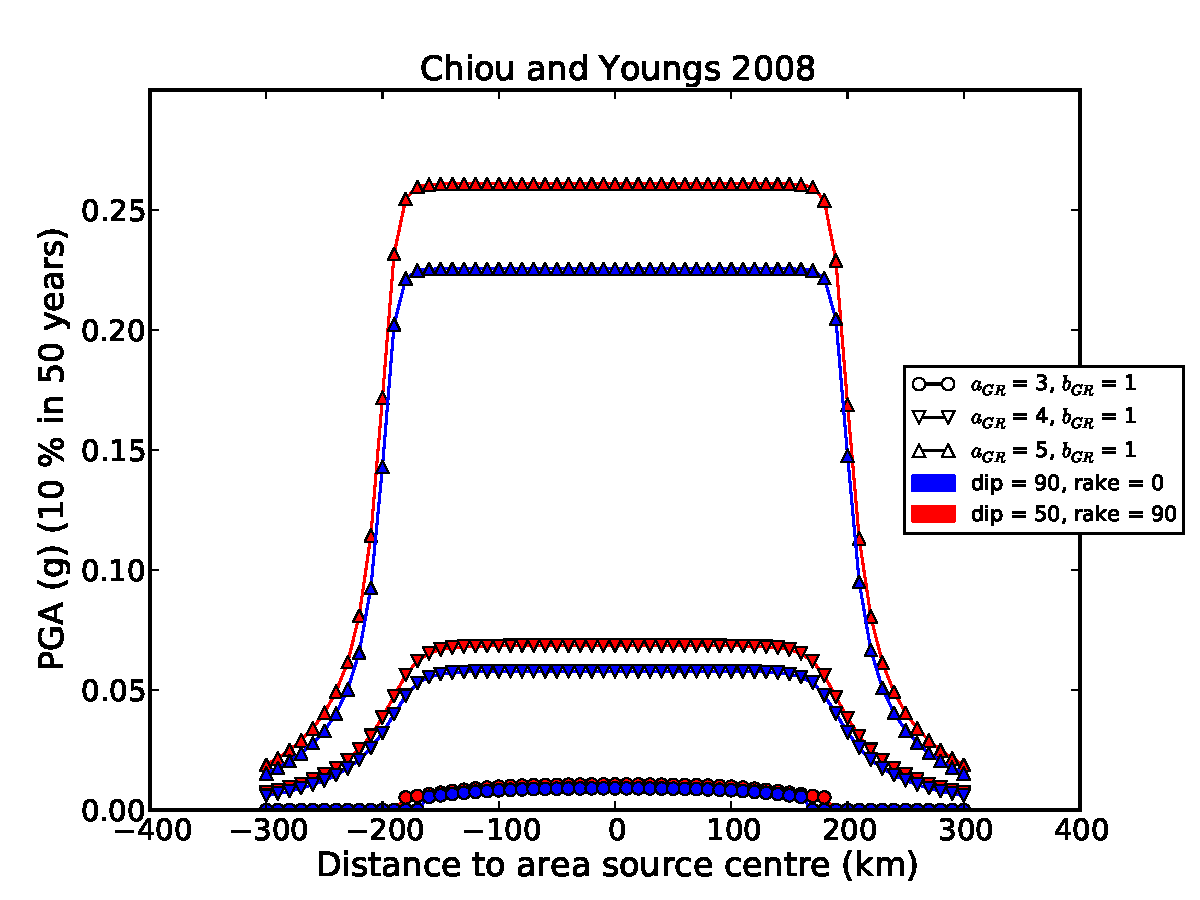
\includegraphics[width=7cm]{./Pictures/PGA_0pt1_CY2008_dip_rake.pdf}
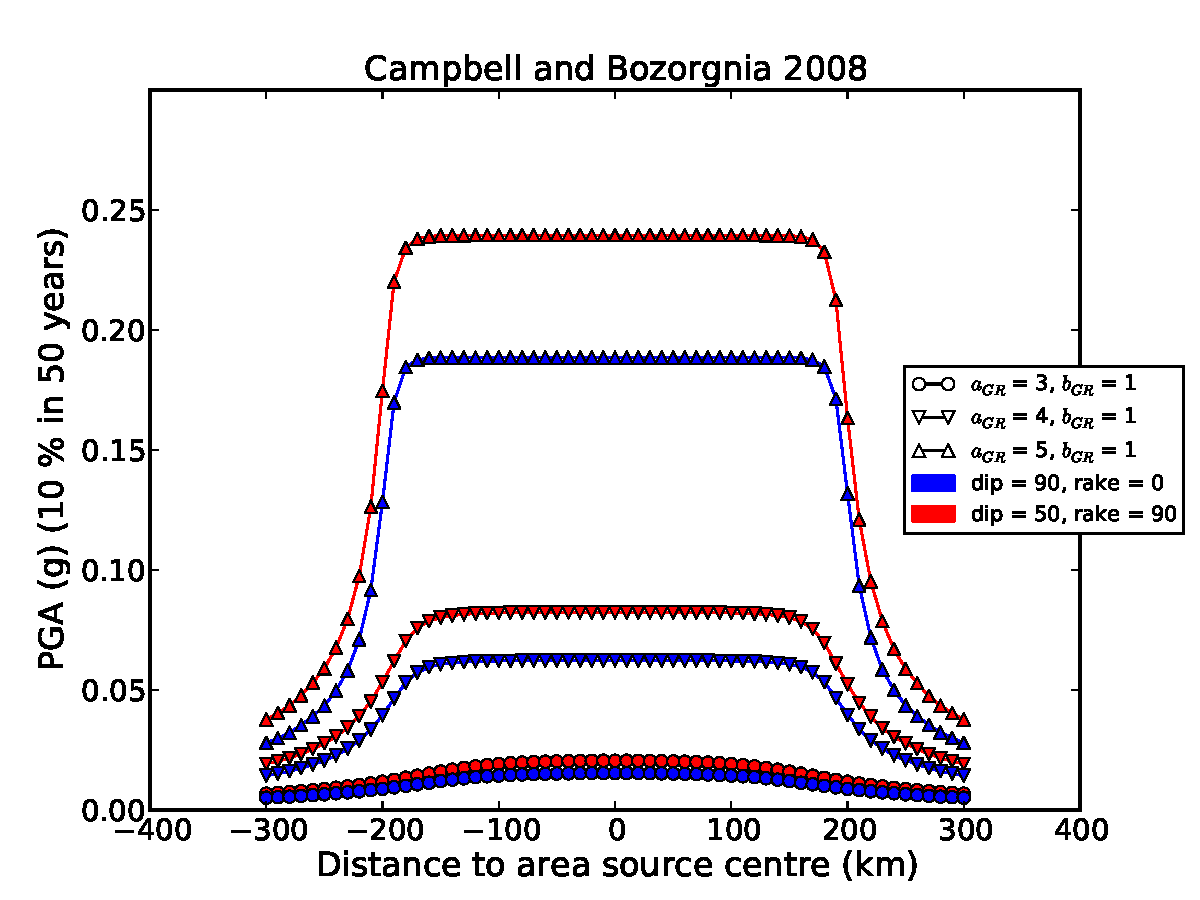
\includegraphics[width=7cm]{./Pictures/PGA_0pt1_CB2008_dip_rake.pdf}
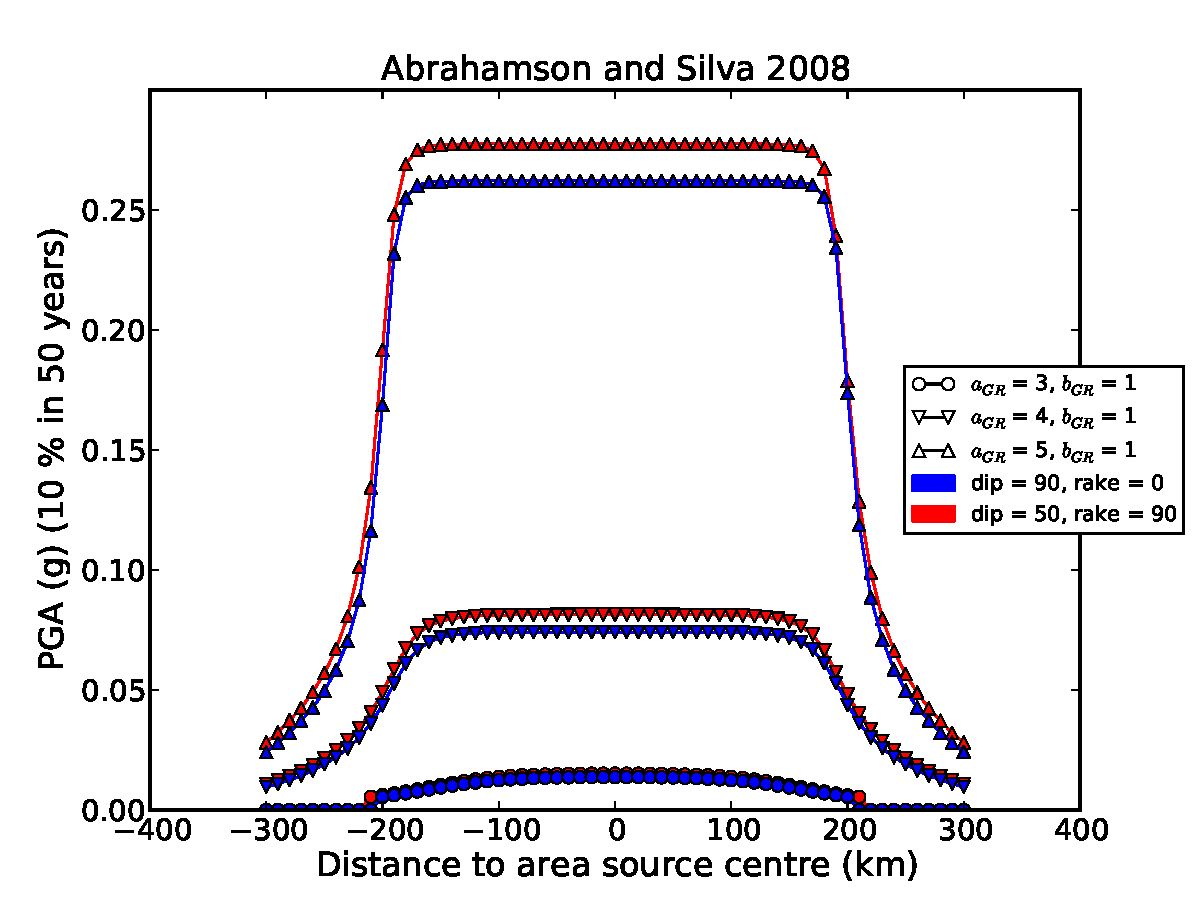
\includegraphics[width=7cm]{./Pictures/PGA_0pt1_AS2008_dip_rake.pdf}
\caption{The effect of dip and rake angles on hazard map calculation.}
\label{fig:dip_rake_area}
\end{figure}

\subsection{The effect of the hypocentral depth distribution}
Another modeling parameter which can influence hazard estimates from an area source is the hypocentral
depth distribution. We show here the effect of considering a single hypocentral depth value (10 km) versus
considering a set of normally distributed values with mean $\mu=10$ km and standard deviation $\sigma=4$ km. By considering the same source-sites configuration as in the previous analysis, and vertical
strike-slip ruptures with single strike ($0^{\circ}$), we compute hazard maps considering two $a_{GR}$ values (4 and 5). We use the GMPE model of \citet{campbell2008}. Figure \ref{fig:hypo_depth_area} shows hazard map values along the site profile for different
return periods (RP) and $a_{GR}$ values. The effect of the distribution of hypocentral values becomes visible when considering long return periods (50000 years) and increases with increasing $a_{GR}$.
\begin{figure}
\centering
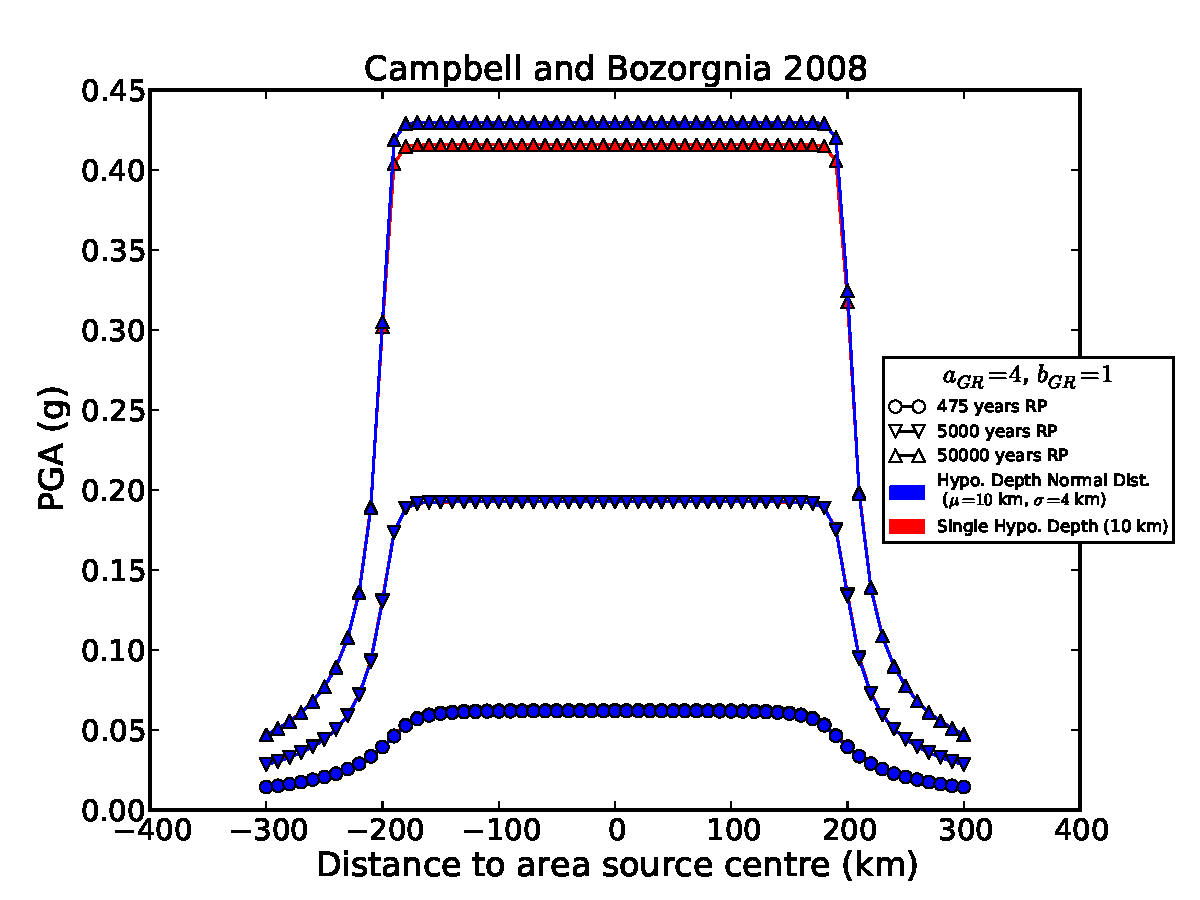
\includegraphics[width=7cm]{./Pictures/PGA_a4_CB2008_hypo_depth.pdf}
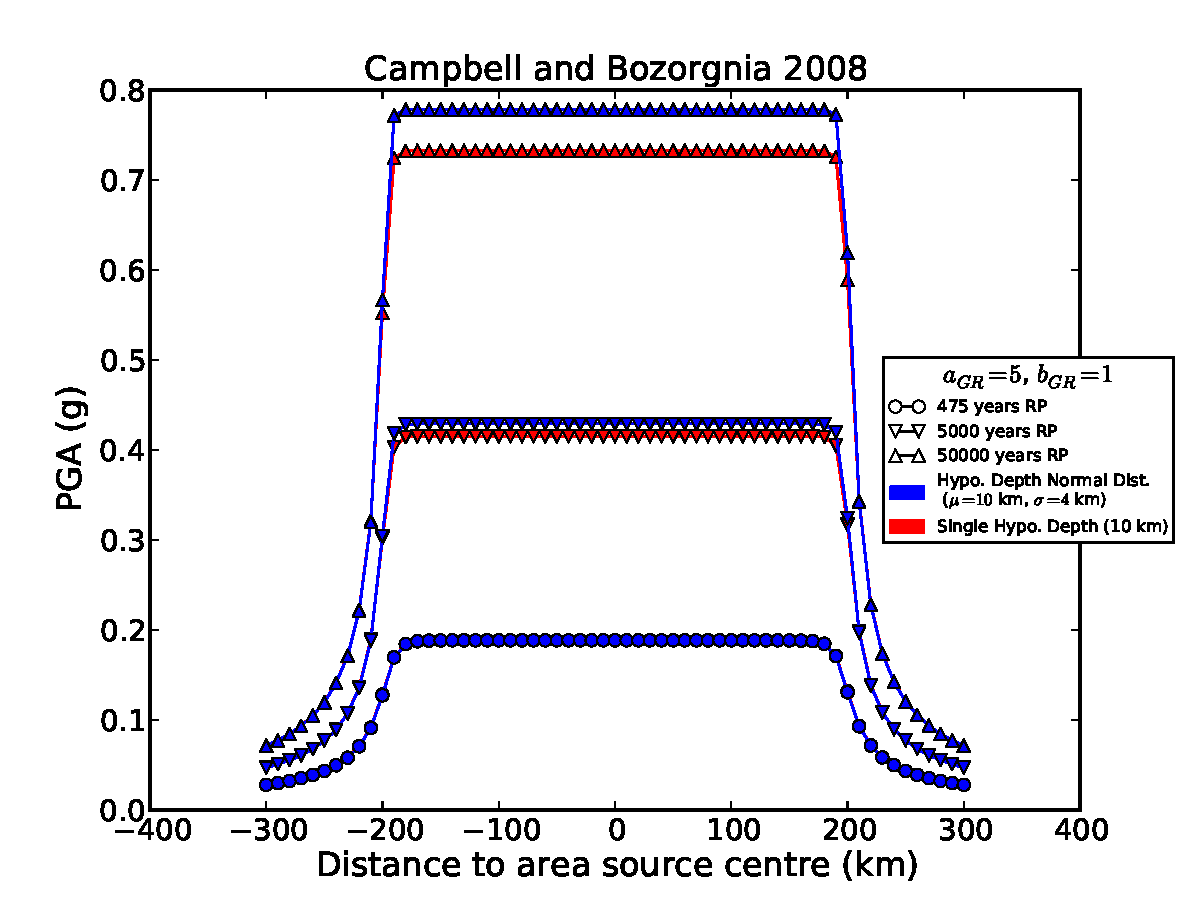
\includegraphics[width=7cm]{./Pictures/PGA_a5_CB2008_hypo_depth.pdf}
\caption{The effect of hypocentral depth on hazard map calculation.}
\label{fig:hypo_depth_area}
\end{figure}


\section{Classical PSHA with complex logic tree}
We consider here a synthetic case of a classical PSHA calculation based on a simple source model consisting of 5 identical area sources. Each source has a square shape of $0.5^{\circ}$ side. Four sources are arranged to form a regular mesh. The fifth source is placed in the middle of the mesh and overlaps with the other
four sources. Each source can have 5 possible ($a_{GR}$, $b_{GR}$) pairs and 3 possible
maximum magnitudes. Assuming the uncertainties to be uncorrelated among sources, the total number of
possible source parameters combinations can be written as:
\begin{align}
N = N_{GR}^{N_{S}} \times N_{MaxMag}^{N_{S}}
\end{align}
where $N_{GR}$ is the number of Gutenberg-Richter parameters (i.e. $a_{GR}$ - $b_{GR}$ pairs) for each
source, $N_{MaxMag}$ is the number of maximum magnitudes for each source, and $N_{S}$ is the number
of sources. In the present case $N_{GR}=5$, $N_{MaxMag}=3$, $N_{S}=5$, and thus $N=5^{5} \times 3^{5}=759375$. $N$ represents the total number of paths in the source model logic tree.

The OQ-engine allows random sampling the logic tree to avoid calculating hazard results for all possible
logic tree paths. Figure \ref{fig:logic_tree_curves} presents mean and quantile hazard curves
as obtained from different numbers of samples (10, 100, 1000, 5000). It can be seen how, by increasing the number
of samples, results tend to converge to similar values. Indeed, curves obtained from 1000 and 5000 samples are almost indistinguishable. The Monte Carlo sampling offers therefore an effective way to reduce the computational burden associated with a large logic tree and to still obtain reliable results. The results reliability can be controlled by performing a convergence analysis; that is by identifying the number of samples
which are required to obtain values that are stable within a certain tolerance level.
\begin{figure}
\centering
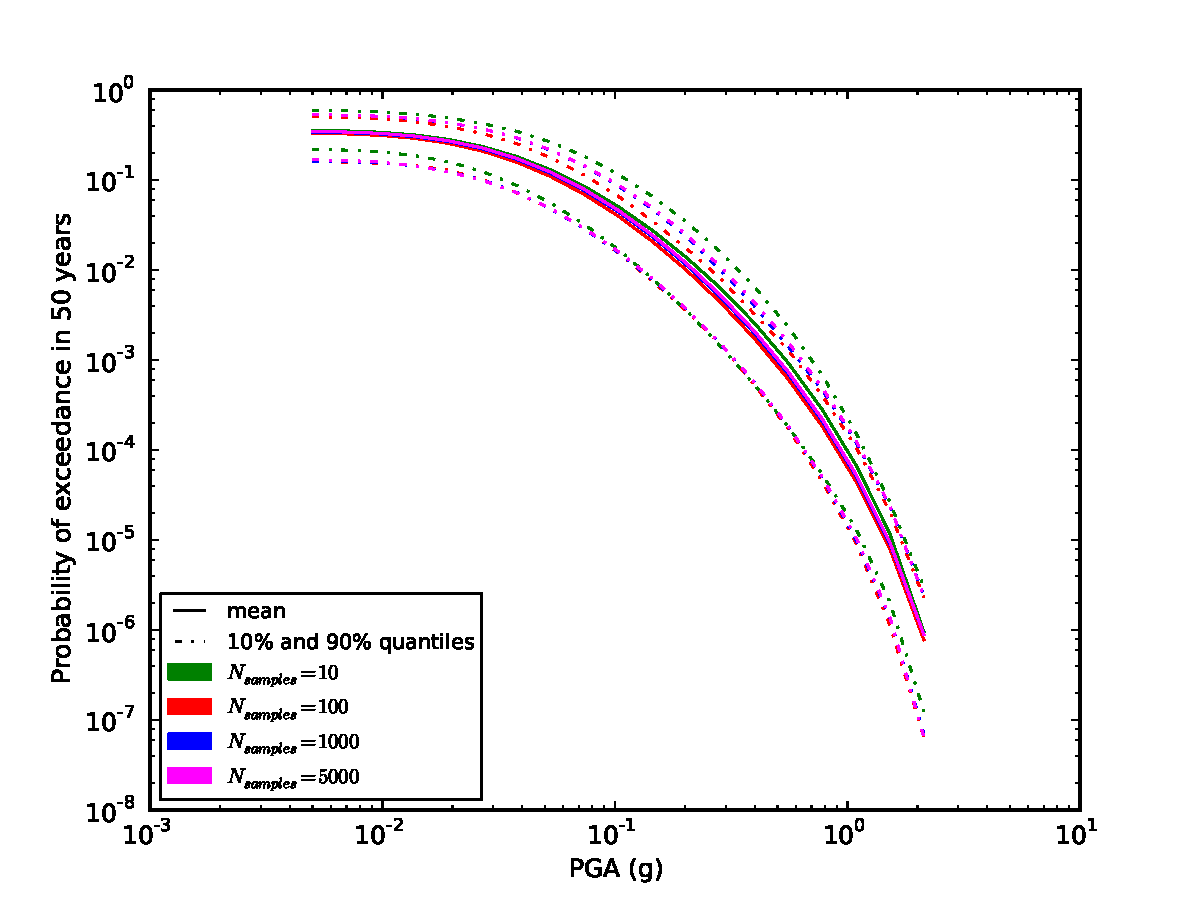
\includegraphics[width=14cm]{./Pictures/LogicTreeCurves.pdf}
\caption{Mean and quantile hazard curves obtained from Monte Carlo sampling of logic tree.}
\label{fig:logic_tree_curves}
\end{figure}

\section{Convergence between Classical and Event-based PSHA}
The event based approach allows generating stochastic event sets and ground motion fields which can then
be used to reproduce the classical results. We present here an event-based calculation for a location corresponding to the city of Seattle. The calculation is done using the 2008 seismic hazard model for conterminous U.S. (\cite{petersen2008}). A stochastic event set corresponding to a duration of 10000
years is generated (Figure \ref{fig:seattle_ses}). The event set contains earthquake ruptures within a radius of
200 km from the city of Seattle (longitude = 122.3W, latitude = 47.6N). The event set includes large subduction interface earthquakes generated in the Cascadia region, as well as deep intraslab and shallow active crust earthquakes. From each event, ground shaking values are simulated in the city of Seattle (considering the full set of GMPEs prescribed by the model). From ground motion values, the mean
hazard curve (probability of exceedance in 50 years) for PGA is computed, and compared against the
one obtained using the classical approach (Figure \ref{fig:seattle_curves}). The curve obtained can reliably
reproduce the probabilities of exceedance down to $10^{-2}$. For lower probabilities a stochastic event
set with longer duration is required.
\begin{figure}
\centering
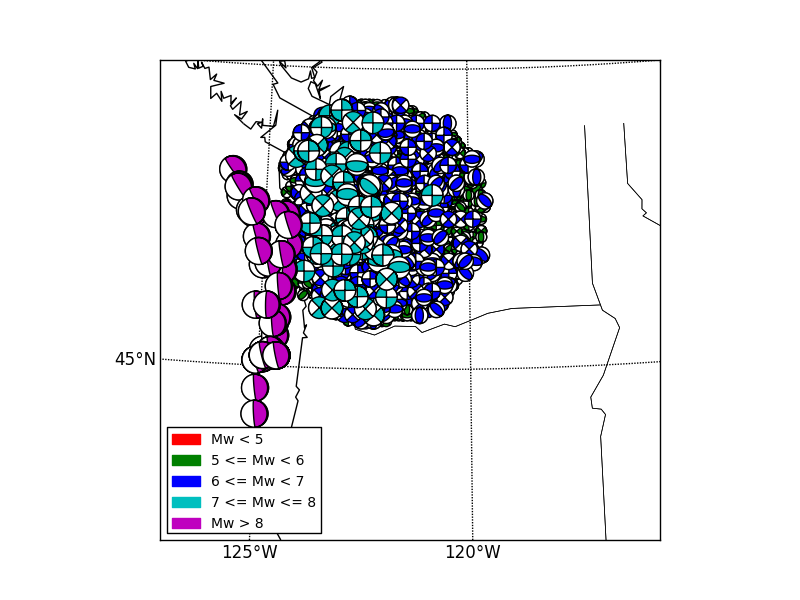
\includegraphics[width=14cm]{./Pictures/ses_USA_NSHMP2008.png}
\caption{Stochastic event set for a region surrounding Seattle (U.S.) for a duration of 10000 years.}
\label{fig:seattle_ses}
\end{figure}
\begin{figure}
\centering
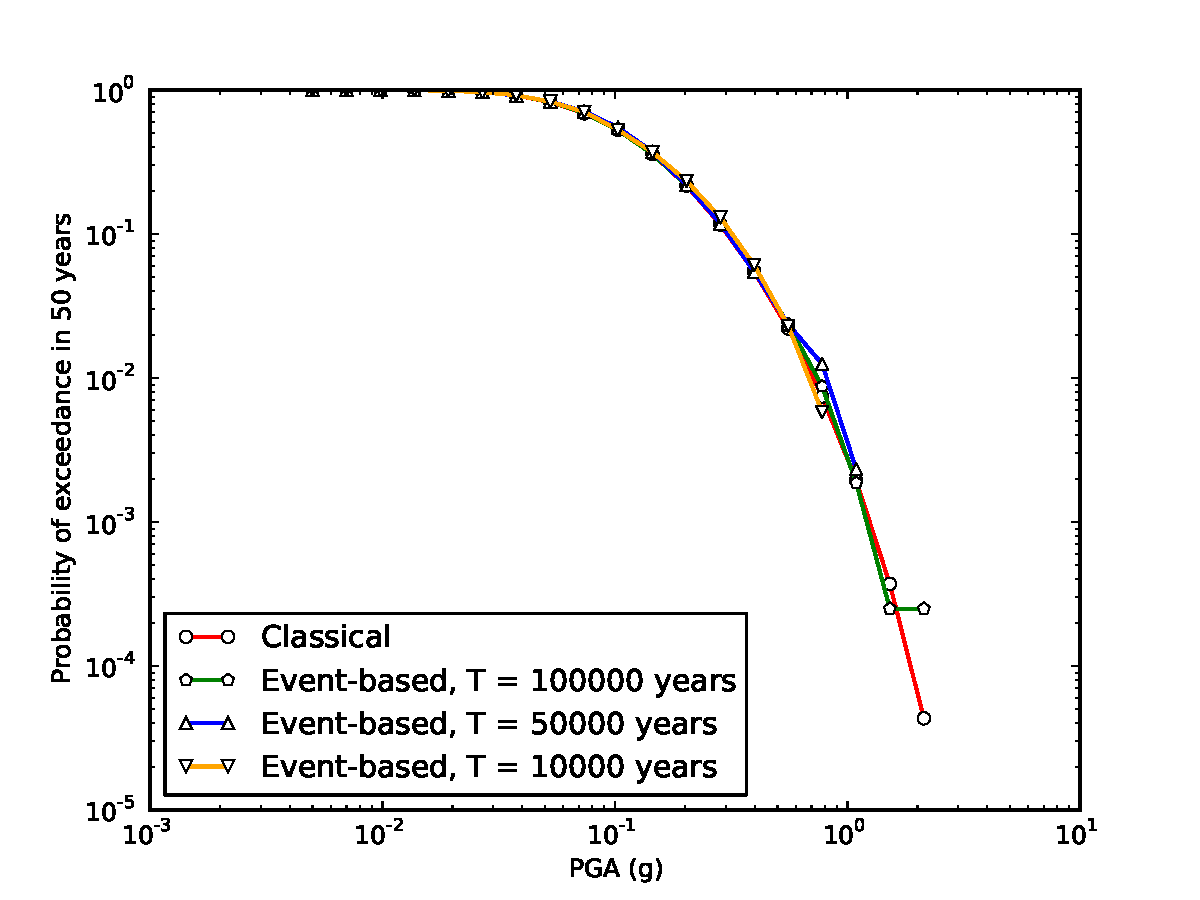
\includegraphics[width=14cm]{./Pictures/Seattle.pdf}
\caption{Hazard curves for Seattle using the Classical and Event-based approaches.}
\label{fig:seattle_curves}
\end{figure}

\section{Disaggregation analysis}
We present here an example of disaggregation analysis for the city of Seattle, always considering the 2008
national seismic hazard model for U.S. developed by \citet{petersen2008}. In particular, we show the geographic-magnitude (Figure \ref{fig:seattle_lonlatmag}) and geographic-tectonic region type (Figure \ref{fig:seattle_lonlattrt}) disaggregation histograms for PGA corresponding to 10\% probability of exceedance in 50 years. The geographic disaggregation allows investigating the spatial distribution of the
seismic sources contributing to a given level of hazard. By including magnitude and tectonic region type,
we can understand the influence of the different tectonic regions, and also the magnitude ranges involved.
Indeed, the disaggregation analysis for the city of Seattle shows that, for a return period of 475 years, the
highest probabilities of ground motion exceedance are associated with active shallow crust events with magnitudes in the range 6 to 7. The second highest contributions are from subduction interface events
with magnitudes above 9. Subduction intraslab events are instead associated to the lowest contributions.
\begin{figure}
\centering
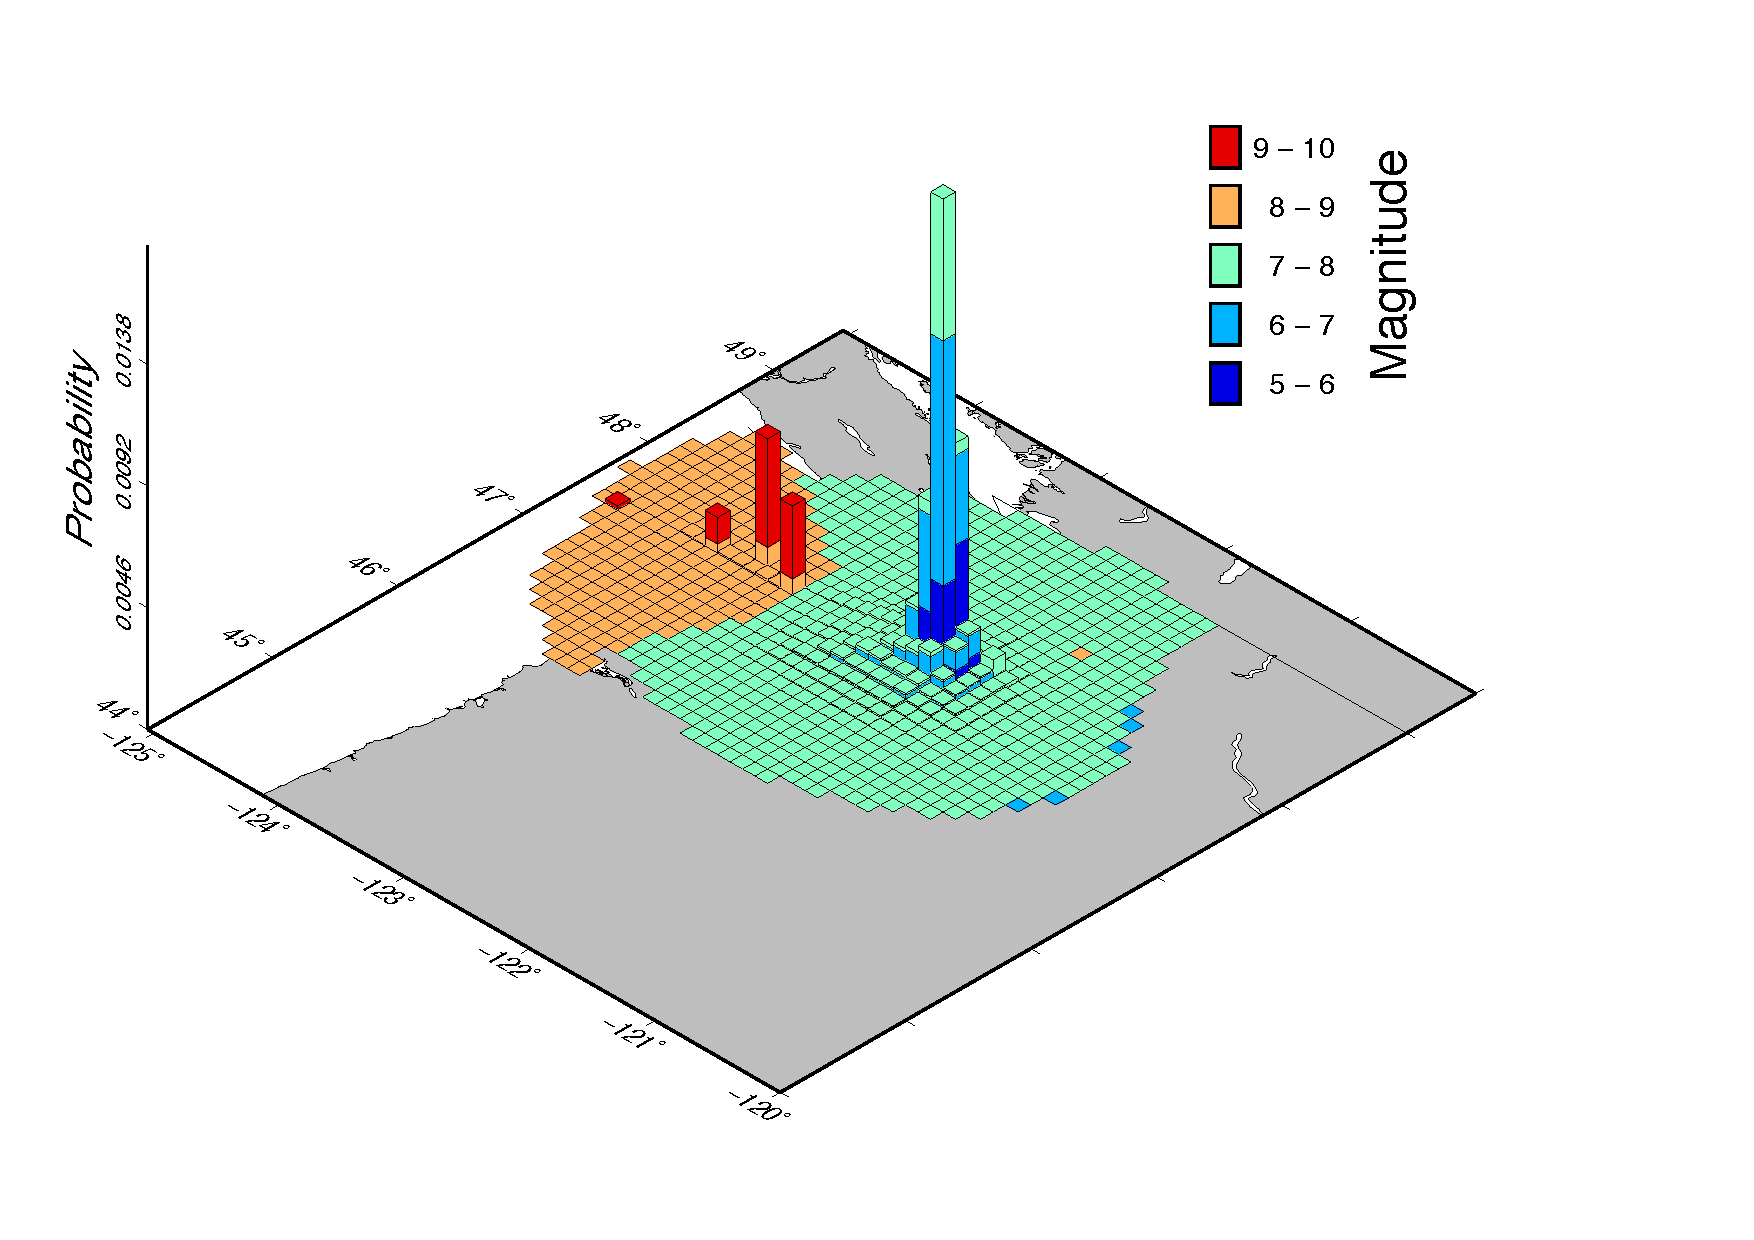
\includegraphics[width=14cm]{./Pictures/Seattle_Lon_Lat_Mag.pdf}
\caption{Longitude, latitude and magnitude disaggregation for PGA corresponding to 10\% probability of exceedance in 50 years.}
\label{fig:seattle_lonlatmag}
\end{figure}

\begin{figure}
\centering
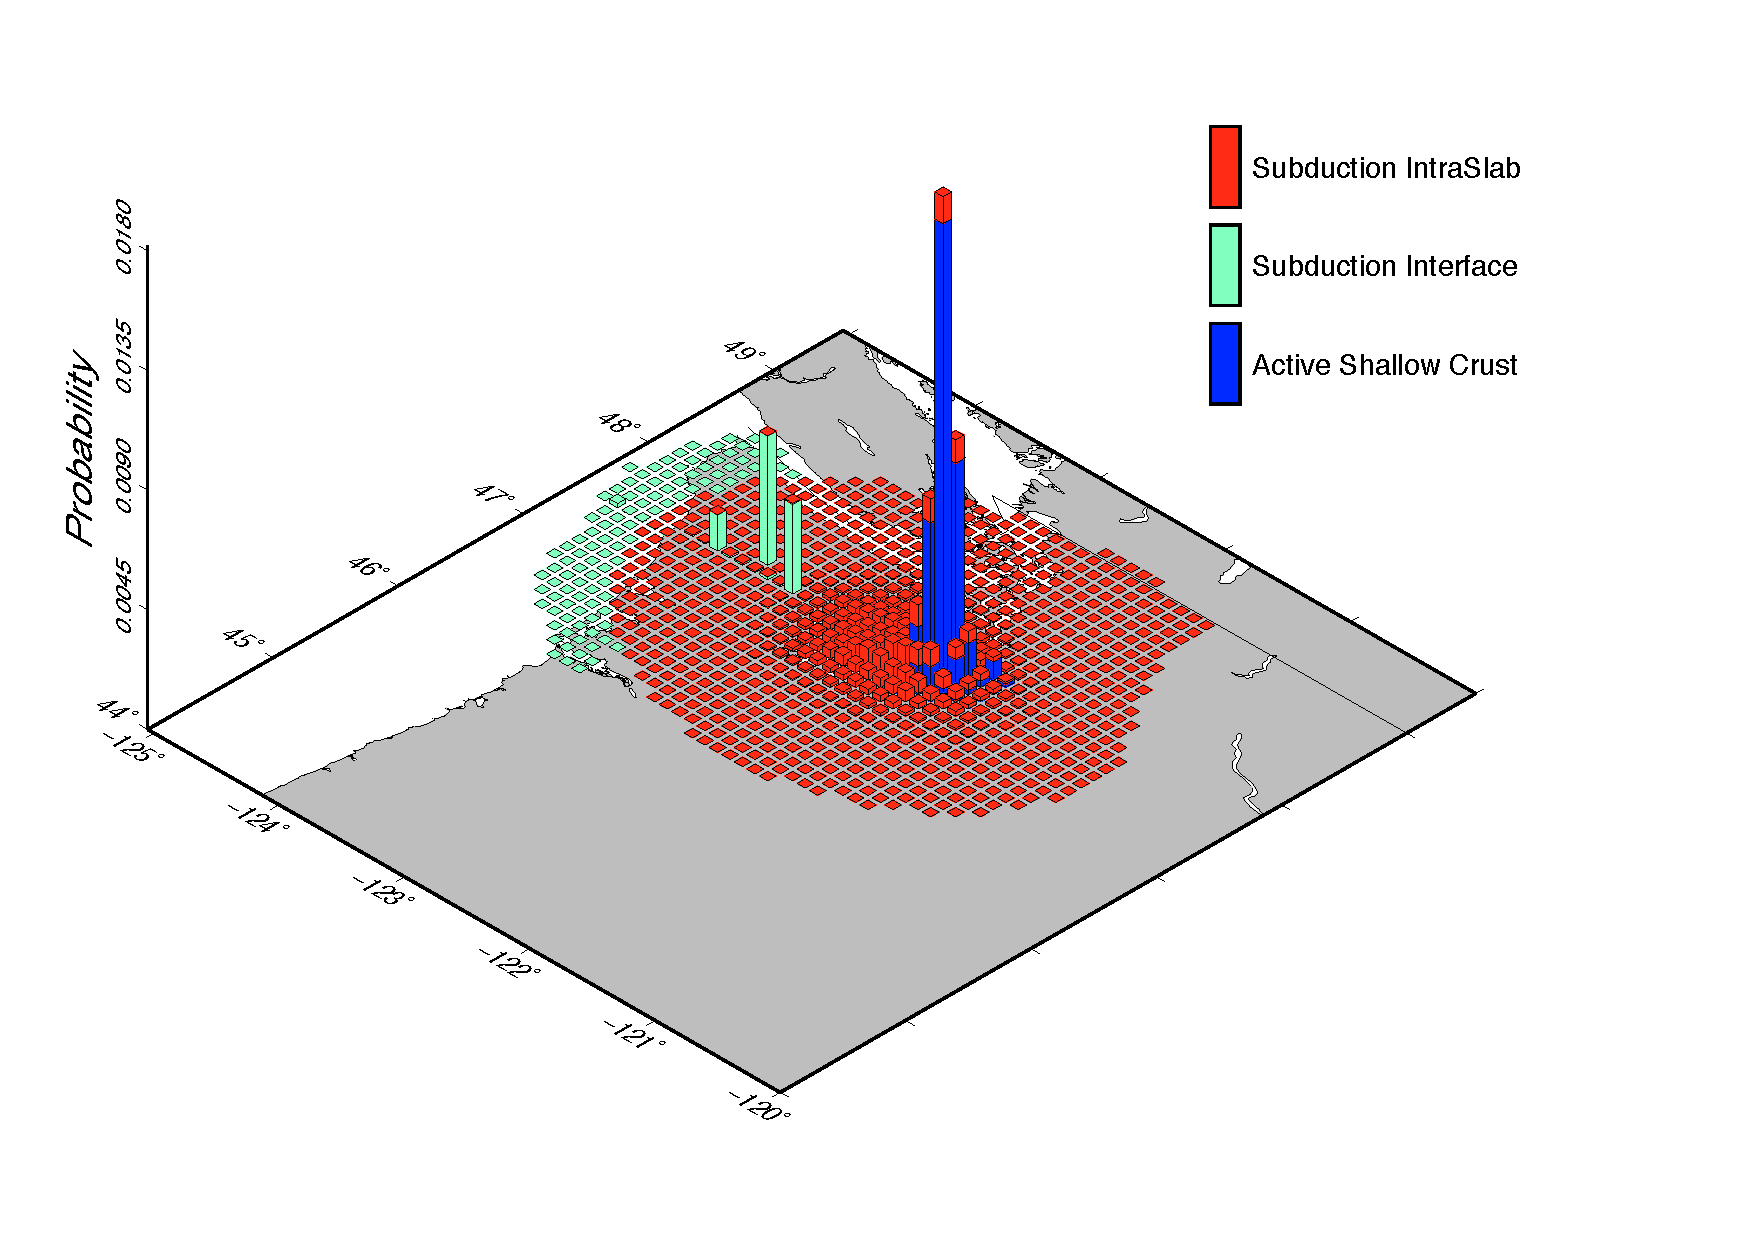
\includegraphics[width=14cm]{./Pictures/Seattle_Lon_Lat_TRT.pdf}
\caption{Longitude, latitude and tectonic region type disaggregation for PGA corresponding to 10\% probability of exceedance in 50 years.}
\label{fig:seattle_lonlattrt}
\end{figure}




%----------------------------------------------------------------------------------------
%	BIBLIOGRAPHY
%----------------------------------------------------------------------------------------
\chapter*{Bibliography}
\addcontentsline{toc}{chapter}{\textcolor{ocre}{Bibliography}}
\section*{Books}
\addcontentsline{toc}{section}{Books}
\printbibliography[heading=bibempty,type=book]
\section*{Articles}
\addcontentsline{toc}{section}{Articles}
\printbibliography[heading=bibempty,type=article]
\section*{Other Sources}
\addcontentsline{toc}{section}{Reports}
\printbibliography[heading=bibempty,nottype=book,nottype=article]


%----------------------------------------------------------------------------------------
%	INDEX
%----------------------------------------------------------------------------------------

\cleardoublepage
\phantomsection
\setlength{\columnsep}{0.75cm}
\addcontentsline{toc}{chapter}{\textcolor{ocre}{Index}}
\printindex
\printglossary

%----------------------------------------------------------------------------------------

\end{document}
